%%%%%%%%%%%%%%%%%%%%%%%%%%%%%%%%%%%%%%%%%%%%%%%%%%%%%%%%%%%%%%%%%%%%%%
% Overleaf (WriteLaTeX) Example: Molecular Chemistry Presentation
%
% Source: http://www.overleaf.com
%
% In these slides we show how Overleaf can be used with standard 
% chemistry packages to easily create professional presentations.
% 
% Feel free to distribute this example, but please keep the referral
% to overleaf.com
% 
%%%%%%%%%%%%%%%%%%%%%%%%%%%%%%%%%%%%%%%%%%%%%%%%%%%%%%%%%%%%%%%%%%%%%%

\documentclass[xcolor={dvipsnames}]{beamer}

\mode<presentation>
{
  \usetheme{Madrid}       % or try default, Darmstadt, Warsaw, ...
  \usecolortheme{default} % or try albatross, beaver, crane, ...
  \usefonttheme{default}    % or try default, structurebold, ...
  \setbeamertemplate{navigation symbols}{}
  \setbeamertemplate{caption}[numbered]
} 

\usepackage[english]{babel}
\usepackage[utf8x]{inputenc}
\usepackage{graphicx}
\usepackage{hyperref}
  \hypersetup{colorlinks=true}
  \hypersetup{urlcolor=blue}
  \hypersetup{linkcolor = .}
\usepackage{xcolor}
\usepackage{siunitx}
  \sisetup{separate-uncertainty = true}
\usepackage{physics}
\usepackage[font=small,labelfont=bf]{caption}
\usepackage{subcaption}
\usepackage[en-GB]{datetime2}
\usepackage{overpic}
\usepackage{feynmp}
\DeclareGraphicsRule{*}{mps}{*}{}
\usepackage{scalerel}
\newcommand{\mylbrace}[2]{\vspace{#2pt}\hspace{6pt}\scaleleftright[\dimexpr5pt+#1\dimexpr0.06pt]{\lbrace}{\rule[\dimexpr2pt-#1\dimexpr0.5pt]{-4pt}{#1pt}}{.}}
\newcommand{\myrbrace}[2]{\vspace{#2pt}\scaleleftright[\dimexpr5pt+#1\dimexpr0.06pt]{.}{\rule[\dimexpr2pt-#1\dimexpr0.5pt]{-4pt}{#1pt}}{\rbrace}\hspace{6pt}}

% Trim in percent
\usepackage{adjustbox}

% No "Figure" prefix
\setbeamertemplate{caption}{\raggedright\insertcaption\par}

% Nice decay amplitude diagrams
\usepackage{amsmath,amssymb,tikz-cd}

% Strike out text
\usepackage[normalem]{ulem}

% For figures with text overlay
\usepackage{overpic}

% Arrows
\usepackage{tikz}
\newcommand{\tikzmark}[1]{\tikz[remember picture] \node[coordinate] (#1) {#1};}

% Colourbox with line breaks
\newcommand{\cbox}[2][lime!20]{%
  \colorbox{#1}{\parbox{\dimexpr\linewidth-2\fboxsep}{\strut #2\strut}}%
}

% Vector arrows
\usepackage[pdftex]{pict2e}

% Checkmark symbol
\def\checkmark{\tikz\fill[scale=0.4](0,.35) -- (.25,0) -- (1,.7) -- (.25,.15) -- cycle;} 

% Here's where the presentation starts, with the info for the title slide
\title[B2OC]{Model-independent determination of \texorpdfstring{$\gamma$}{gamma} with \texorpdfstring{$B^\pm\to[h^+h^-\pi^+\pi^-]_Dh^\pm$}{B2DhD2hhpipi} in phase-space bins}

\author[Martin Tat]{Martin Tat}
\institute[University of Oxford]{\normalsize University of Oxford\\ \vspace{0.3cm}\normalsize B2OC meeting}
\date{4th April 2024}

\titlegraphic{
\includegraphics[height = 2.3cm]{lhcb.jpg}\hspace{1.5cm}~%
              
\includegraphics[height = 2.3cm]{OxfordLogo.pdf}}

\begin{document}

\begin{frame}
  \titlepage
\end{frame}

% These three lines create an automatically generated table of contents.
% \begin{frame}{Outline}
%   \tableofcontents
% \end{frame}

\section{Introduction to \texorpdfstring{$\gamma$}{gamma} and \texorpdfstring{$C\!P$}{CP} violation}
\begin{frame}{Introduction to $\gamma$ and $C\!P$ violation}
  \begin{itemize}
    \setlength\itemsep{0.3em}
    \item{CPV in SM is described by the Unitary Triangle, with angles $\alpha$, $\beta$, $\gamma$}
    \item{The angle $\gamma = \text{arg}\Big(-\frac{V^{\phantom{*}}_{ud}V^*_{ub}}{V^{\phantom{*}}_{cd}V^*_{cb}}\Big)$ is very important:}
    \begin{enumerate}
    \setlength\itemsep{0.2em}
      \item{Negligible theoretical uncertainties: Ideal SM benchmark}
      \item{Accessible at tree level: Indirectly probe New Physics that enter loops}
      \item{Compare with a global CKM fit: Is the Unitary Triangle a triangle?}
    \end{enumerate}
  \end{itemize}
  \vspace{-0.2cm}
  \begin{figure}
    \centering
    \begin{subfigure}{0.5\textwidth}
      \centering
      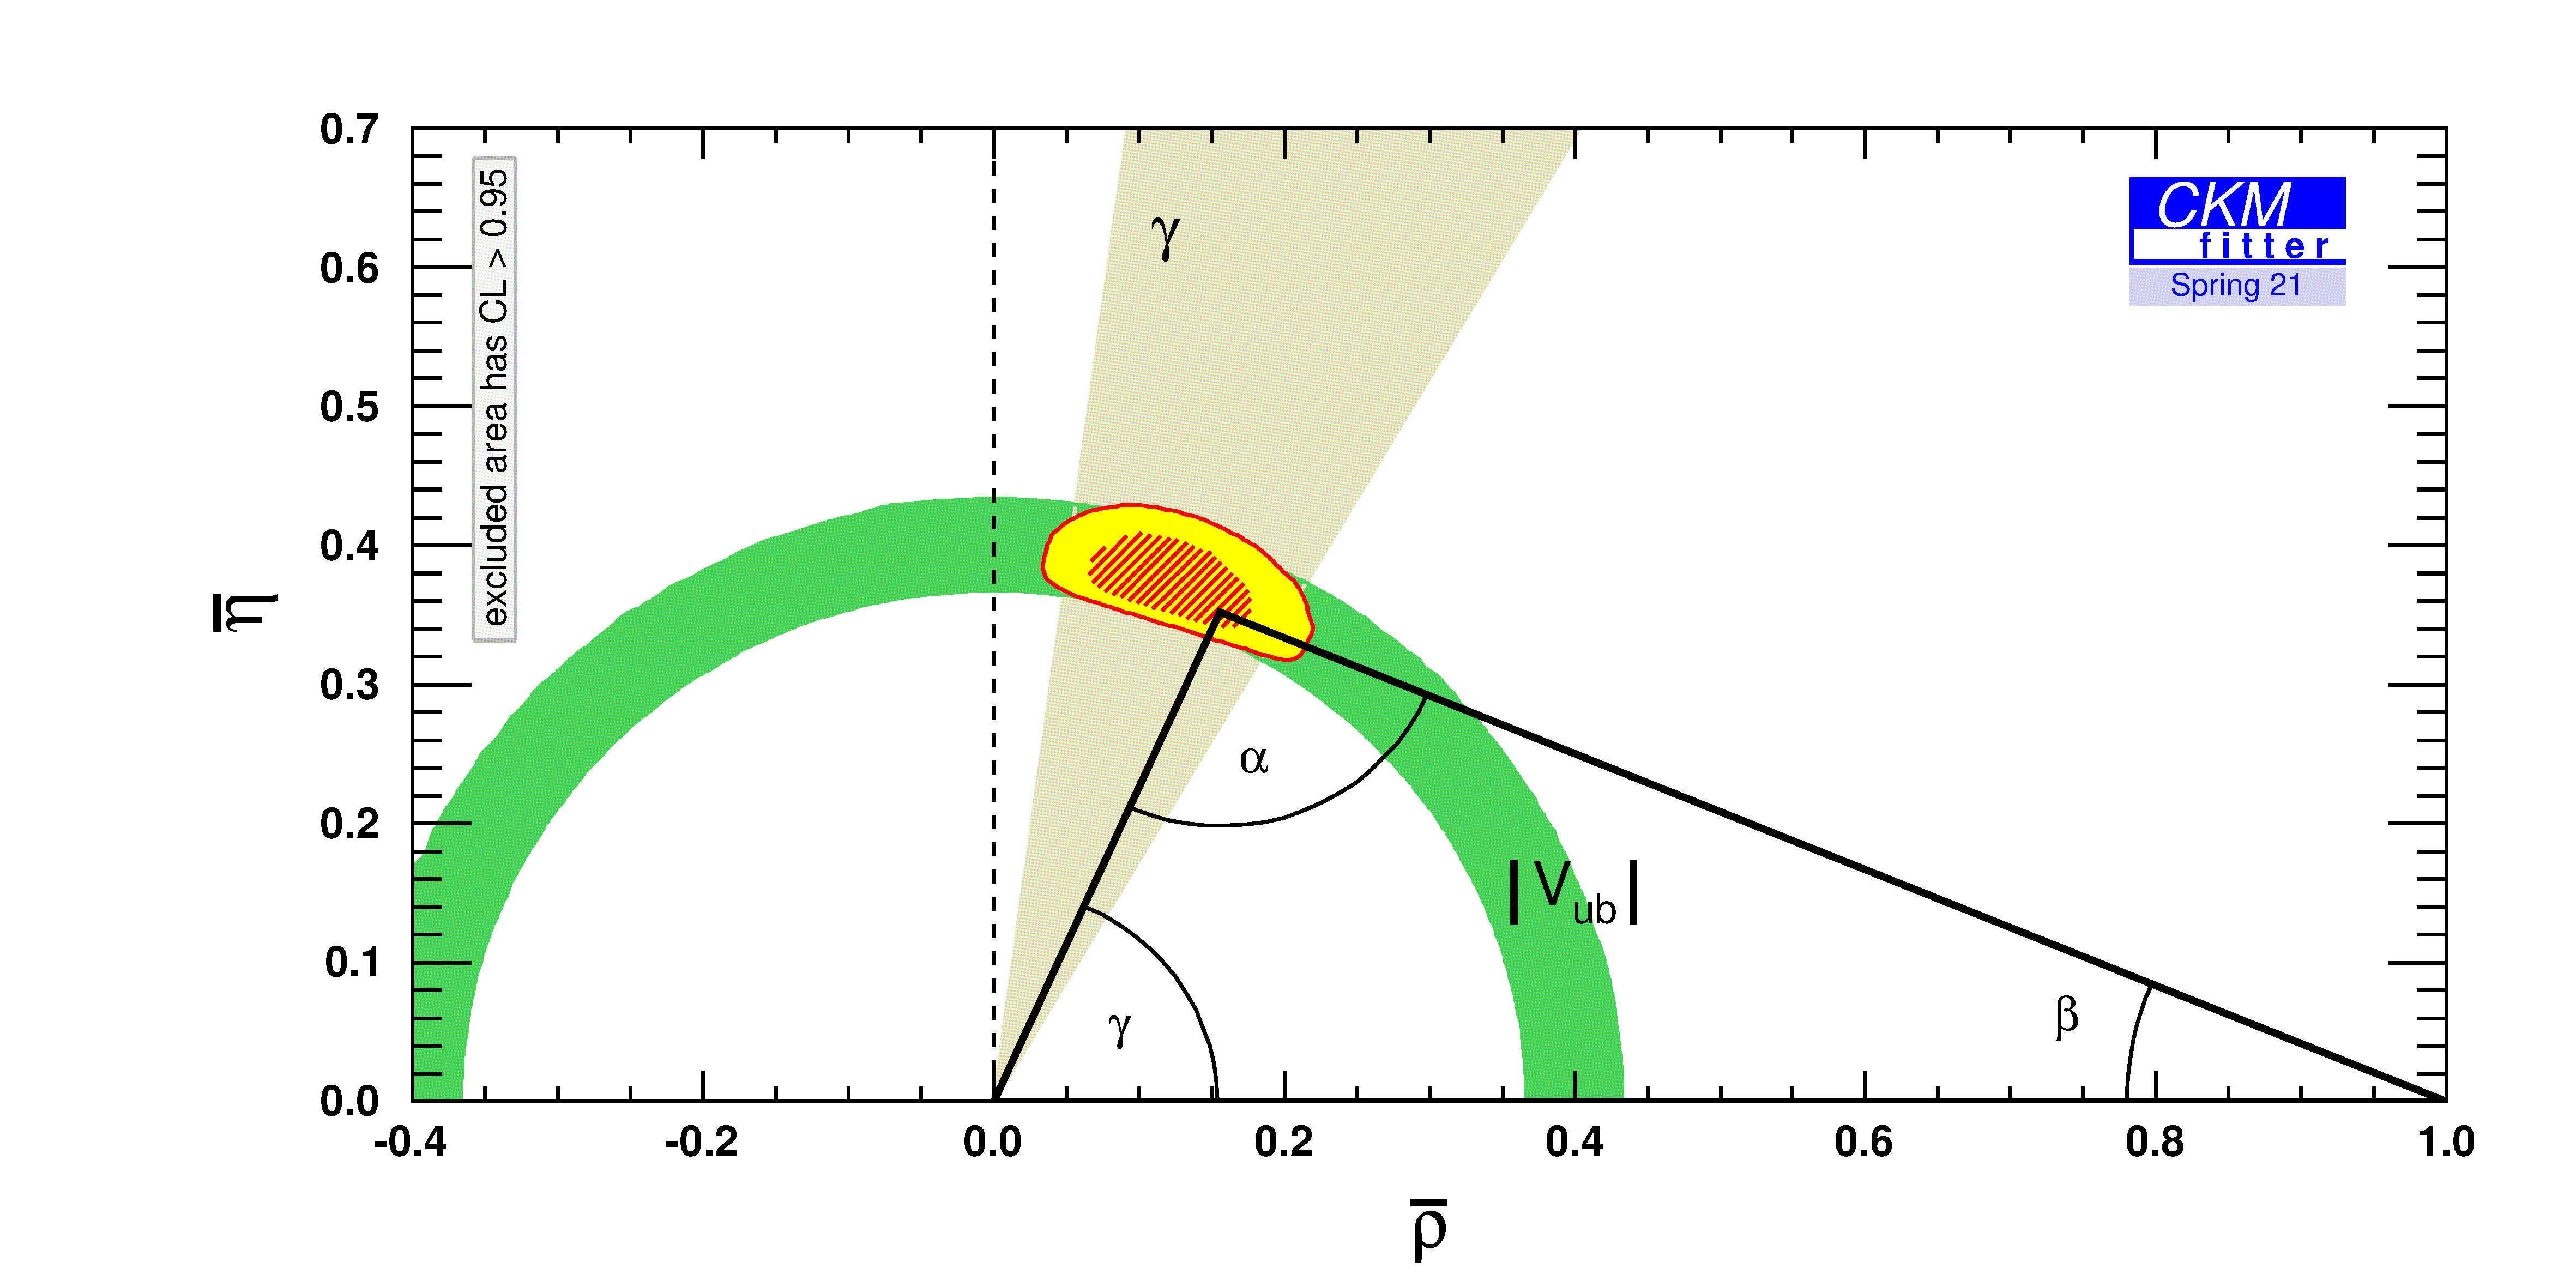
\includegraphics[width = 1.0\textwidth]{Plots/ckmfitter_tree.png}
      \caption{Tree level: $\gamma = \big(72.1^{+5.4}_{-5.7}\big)^\circ$}
    \end{subfigure}%
    \begin{subfigure}{0.5\textwidth}
      \centering
      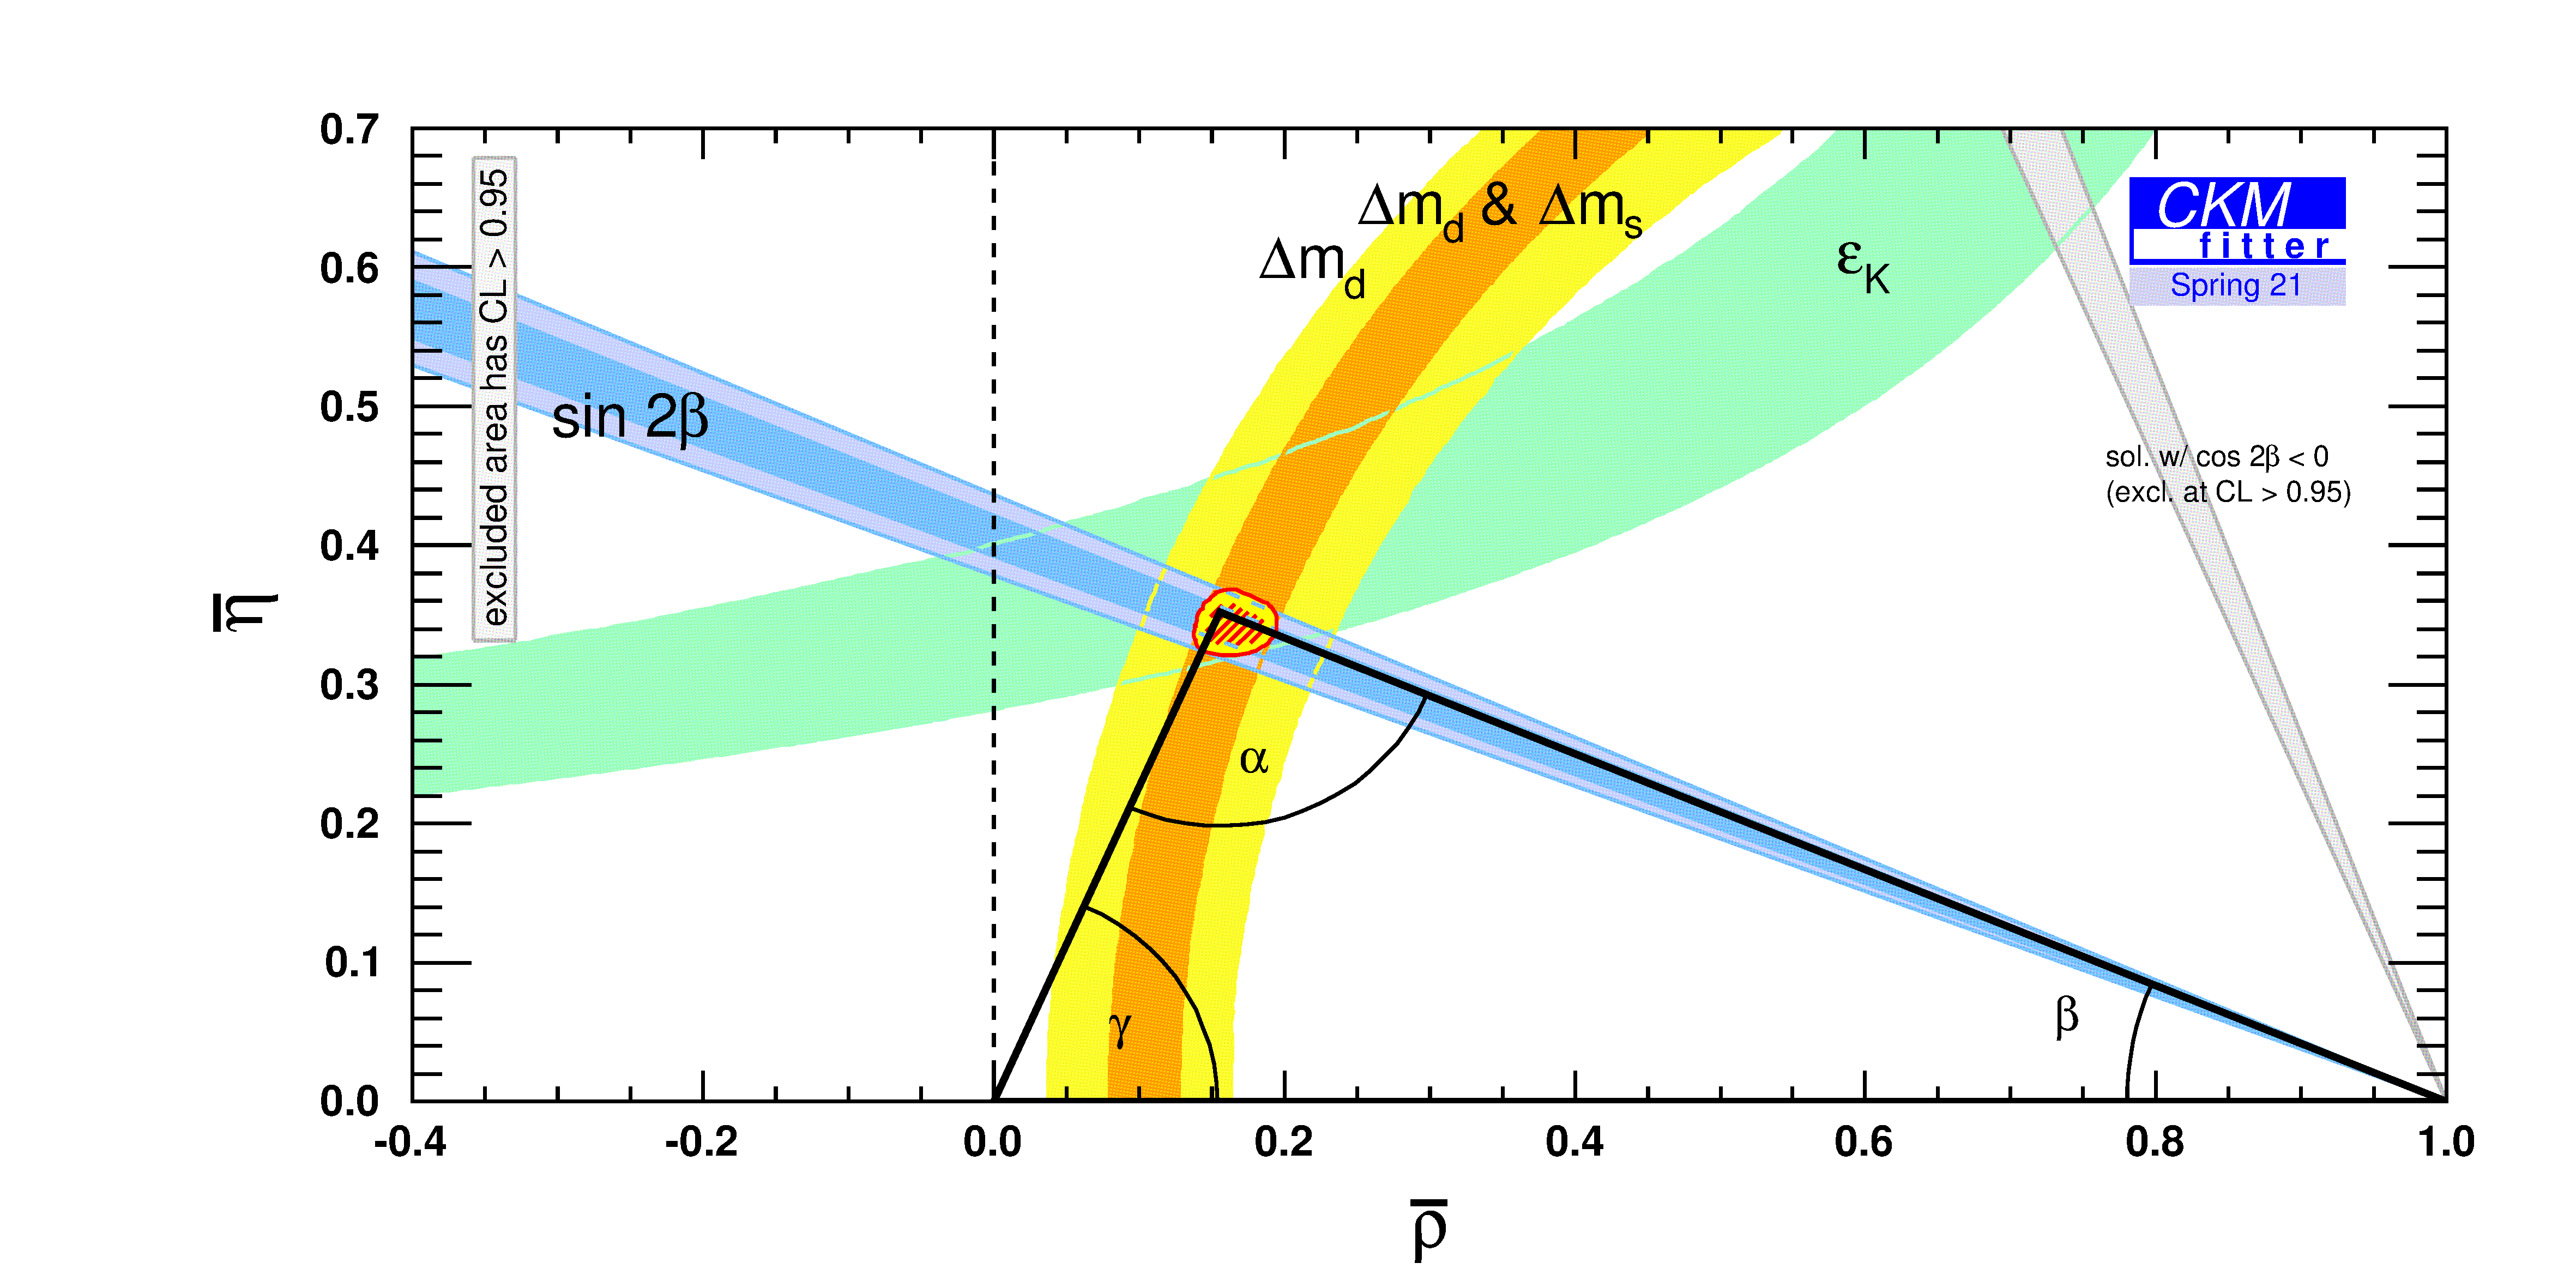
\includegraphics[width = 1.0\textwidth]{Plots/ckmfitter_loop.png}
      \caption{Loop level: $\gamma = \big(65.5^{+1.1}_{-2.7}\big)^\circ$}
    \end{subfigure}
    \vspace{-0.3cm}
    \captionsetup{justification=centering}
    \caption*{\centering\tiny CKMfitter Group (J. Charles et al.), Eur. Phys. J. C41, 1-131 (2005), updated results and plots available at: \href{http://ckmfitter.in2p3.fr}{http://ckmfitter.in2p3.fr}}
  \end{figure}
\end{frame}

\begin{frame}{Sensitivity through interference}
  \begin{center}
    \Large Measure $\gamma$ through interference effects in $B^\pm\to DK^\pm$
  \end{center}
  \begin{figure}[H]
    \centering
    \begin{subfigure}{0.5\textwidth}
      \centering
      \begin{fmffile}{fgraph/fgraph_BtoDK1}
        \setlength{\unitlength}{0.4cm}
        \begin{fmfgraph*}(6,6)
          \fmfstraight
          \fmfleft{i1,B,i2,t1,t2,t3,t9,t10}
          \fmfright{o1,D,o2,t4,t5,o3,K,o4}
          \fmflabel{$\bar{u}$}{i1}
          \fmflabel{$b$}{i2}
          \fmfv{l.d=20,l.a=180,l={$B^-$\mylbrace{30}{-8}}}{B}
          \fmflabel{$\bar{u}$}{o1}
          \fmflabel{$c$}{o2}
          \fmflabel{$\bar{u}$}{o3}
          \fmflabel{$s$}{o4}
          \fmfv{l.d=15,l.a=0,l={\myrbrace{30}{-12}}$D^0$}{D}
          \fmfv{l.d=15,l.a=0,l={\myrbrace{30}{11}}$K^-$}{K}
          \fmf{fermion}{o1,i1}
          \fmf{fermion,tension=1.5}{i2,v1}
          \fmf{fermion}{v1,o2}
          \fmf{phantom,tension=1.5}{t9,v2}
          \fmf{boson,label=$W$,label.side=left,tension=0}{v1,v2}
          \fmf{fermion}{v2,o4}
          \fmf{fermion}{o3,v2}
        \end{fmfgraph*}
      \end{fmffile}
      \vspace{0.5cm}
      \caption*{Favoured $B^-\to D^0K^-$}
    \end{subfigure}%
    \begin{subfigure}{0.5\textwidth}
      \centering
      \begin{fmffile}{fgraph/fgraph_BtoDK2}
        \setlength{\unitlength}{0.4cm}
        \begin{fmfgraph*}(6,6)
          \fmfstraight
          \fmfleft{i1,t1,t2,B,t9,t10,i2}
          \fmfright{o1,K,o2,t4,t5,o3,D,o4}
          \fmflabel{$\bar{u}$}{i1}
          \fmflabel{$b$}{i2}
          \fmfv{l.d=20,l.a=180,l={$B^-$\mylbrace{100}{-8}}}{B}
          \fmflabel{$\bar{u}$}{o1}
          \fmflabel{$s$}{o2}
          \fmflabel{$\bar{c}$}{o3}
          \fmflabel{$u$}{o4}
          \fmfv{l.d=15,l.a=0,l={\myrbrace{30}{13}}$\bar{D^0}$}{D}
          \fmfv{l.d=15,l.a=0,l={\myrbrace{30}{-13}}$K^-$}{K}
          \fmf{fermion}{o1,i1}
          \fmf{fermion,tension=1.5}{i2,v1}
          \fmf{fermion}{v1,o4}
          \fmf{phantom,tension=1.5}{t2,v2}
          \fmf{boson,label=$W$,label.side=left,tension=0}{v1,v2}
          \fmf{fermion}{v2,o2}
          \fmf{fermion}{o3,v2}
        \end{fmfgraph*}
      \end{fmffile}
      \vspace{0.5cm}
      \caption*{Suppressed $B^-\to\bar{D^0}K^-$}
    \end{subfigure}
  \end{figure}
  \vspace{-0.3cm}
  \begin{itemize}
    \item{Superposition of $D^0$ and $\bar{D^0}$}
    \begin{itemize}
      \item{Consider $D^0$/$\bar{D^0}$ decays to the same final state, such as $D\to K^+K^-$}
    \end{itemize}
    \item{$b\to u\bar{c}s$ and $b\to c\bar{u}s$ interference $\to$ Sensitivity to $\gamma$}
  \end{itemize}
  \vspace{-0.3cm}
  \begin{center}
    $\mathcal{A}(B^-)=\mathcal{A}_B\Big(\mathcal{A}_{D^0} + r_Be^{i(\delta_B - \gamma)}\mathcal{A}_{\bar{D^0}}\Big)$ \\
    $\mathcal{A}(B^+)=\mathcal{A}_B\Big(\mathcal{A}_{\bar{D^0}} + r_Be^{i(\delta_B + \gamma)}\mathcal{A}_{D^0}\Big)$ \\
  \end{center}
\end{frame}

\begin{frame}[fragile]{Multi-body $D$ decays}
  \begin{center}
    This talk: Discuss $D\to K^+K^-\pi^+\pi^-$, where interference effects vary across phase space
  \end{center}
  \vspace{-0.3cm}
  \begin{itemize}
    \setlength\itemsep{0.5em}
    \item{Strong-phase difference $\delta_D$ is a function of phase space}
    \item{Compare yields of $B^+$ and $B^-$ and determine the asymmetry \underline{in local phase space regions}, known as phase-space bins}
  \end{itemize}
  \begin{equation*}
    \begin{tikzcd}[column sep=huge]
      & D^0K^- \arrow[dr, bend left = 25, "\mathcal{A}_{D^0}(\Phi)"] & \\
      B^- \arrow[ur, bend left, "\mathcal{A}_B"] \arrow[dr, bend right, "\mathcal{A}_B r_B e^{i(\delta_B - \gamma)}"'] & [5cm] & DK^- \\
      & \bar{D^0}K^- \arrow[ur, bend right = 25, "\mathcal{A}_{\bar{D^0}}(\Phi)"'] & \\
    \end{tikzcd}
  \end{equation*}
  \vspace{-0.9cm}
  \begin{align*}
    \lvert\mathcal{A}(B^-)\lvert^2&\propto\lvert\mathcal{A}_{D^0}(\Phi)\lvert^2 + r_B^2\lvert\mathcal{A}_{\bar{D^0}}(\Phi)\lvert^2 \\
    &+ 2r_B\lvert\mathcal{A}_{D^0}(\Phi)\lvert\lvert\mathcal{A}_{\bar{D^0}}(\Phi)\lvert\cos(\delta_B - \gamma + \delta_D)
  \end{align*}
\end{frame}

\begin{frame}{The BPGGSZ method}
\begin{center}
    \begin{minipage}{0.6\textwidth}
      \begin{block}{Event yield in bin $i$}
        \footnotesize
        $N^-_i = h_{B^-}\big(F_i + (x_-^2 + y_-^2)\bar{F_i} + 2\sqrt{F_i\bar{F_i}}(x_-c_i + y_-s_i)\big)$ \\
        $N^+_{-i} = h_{B^+}\big(F_i + (x_+^2 + y_+^2)\bar{F_i} + 2\sqrt{F_i\bar{F_i}}(x_+c_i + y_+s_i)\big)$
      \end{block}
    \end{minipage}
  \end{center}
  \begin{itemize}
    \item{CP observables:}
    \begin{itemize}
      \item{$x_\pm^{DK} = r_B^{DK}\cos(\delta_B^{DK}\pm\gamma)$, \quad $y_\pm^{DK} = r_B^{DK}\sin(\delta_B^{DK}\pm\gamma)$}
      \item{$x_\xi^{D\pi} = \Re(\xi^{D\pi})$, $y_\xi^{D\pi} = \Im(\xi^{D\pi})$ $\quad\quad\Big(\xi^{D\pi} = \frac{r_B^{D\pi}}{r_B^{DK}}e^{i(\delta_B^{D\pi} - \delta_B^{DK})}\Big)$}
    \end{itemize}
    \item{Fractional bin yield:}
    \begin{itemize}
      \item{$F_i = \frac{\int_i\dd{\Phi}|\mathcal{A}(D^0)|^2}{\sum_j\int_j\dd{\Phi}\abs{\mathcal{A}(D^0)}^2}$}
      \item{Floated in the fit, mostly constrained by $B^\pm\to D\pi^\pm$}
    \end{itemize}
  \end{itemize}
  \begin{itemize}
    \item{Amplitude averaged strong phases:}
    \begin{center}
      $c_i = \frac{\int_i\dd{\Phi}|\mathcal{A}(D^0)||\mathcal{A}(\bar{D^0})|\cos(\delta_D)}{\sqrt{\int_i\dd{\Phi}\abs{\mathcal{A}(D^0)}^2\int_i\dd{\Phi}\abs{\mathcal{A}(\bar{D^0})}^2}}$ \quad $s_i = \frac{\int_i\dd{\Phi}|\mathcal{A}(D^0)||\mathcal{A}(\bar{D^0})|\sin(\delta_D)}{\sqrt{\int_i\dd{\Phi}\abs{\mathcal{A}(D^0)}^2\int_i\dd{\Phi}\abs{\mathcal{A}(\bar{D^0})}^2}}$
    \end{center}
  \end{itemize}
\end{frame}

\section{Model-dependent \texorpdfstring{$\gamma$}{gamma} with \texorpdfstring{$D\to K^+K^-\pi^+\pi^-$}{D2KKpipi}}
\begin{frame}{$D^0\to K^+K^-\pi^+\pi^-$ binning scheme}
  \begin{itemize}
    \setlength\itemsep{0.5em}
    \item{Interpretation of $\gamma$ from the multi-body charm decays require external inputs of the charm strong-phase differences}
    \item{Measure model-independent strong-phases at a charm factory, such as BESIII, using an optimised binning scheme}
  \end{itemize}
  \begin{figure}
    \centering
    \begin{subfigure}{0.5\textwidth}
      \centering
      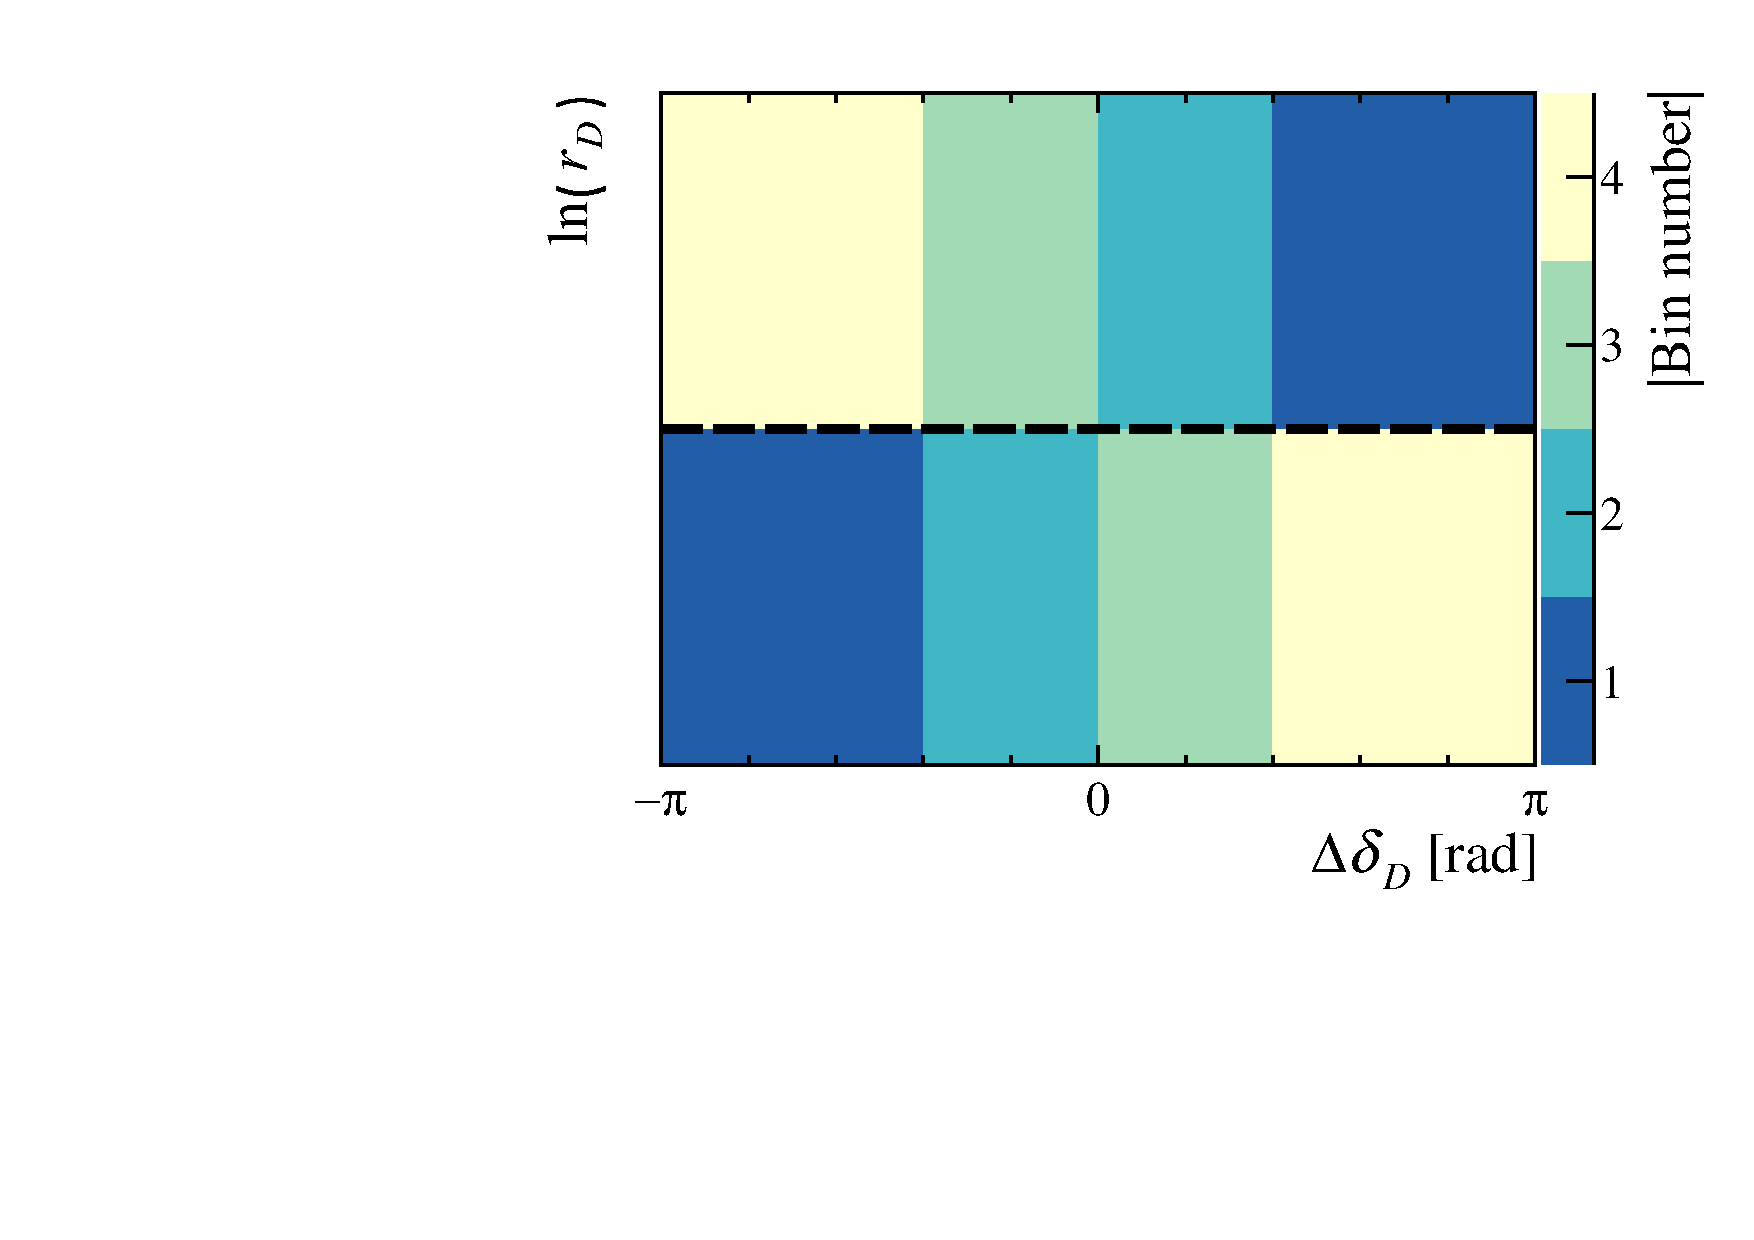
\includegraphics[height = 3.5cm]{Plots/BinningSchemePlot_4Bins.pdf}
      \vspace{-0.3cm}
      \caption*{4 bins}
    \end{subfigure}%
    \begin{subfigure}{0.5\textwidth}
      \centering
      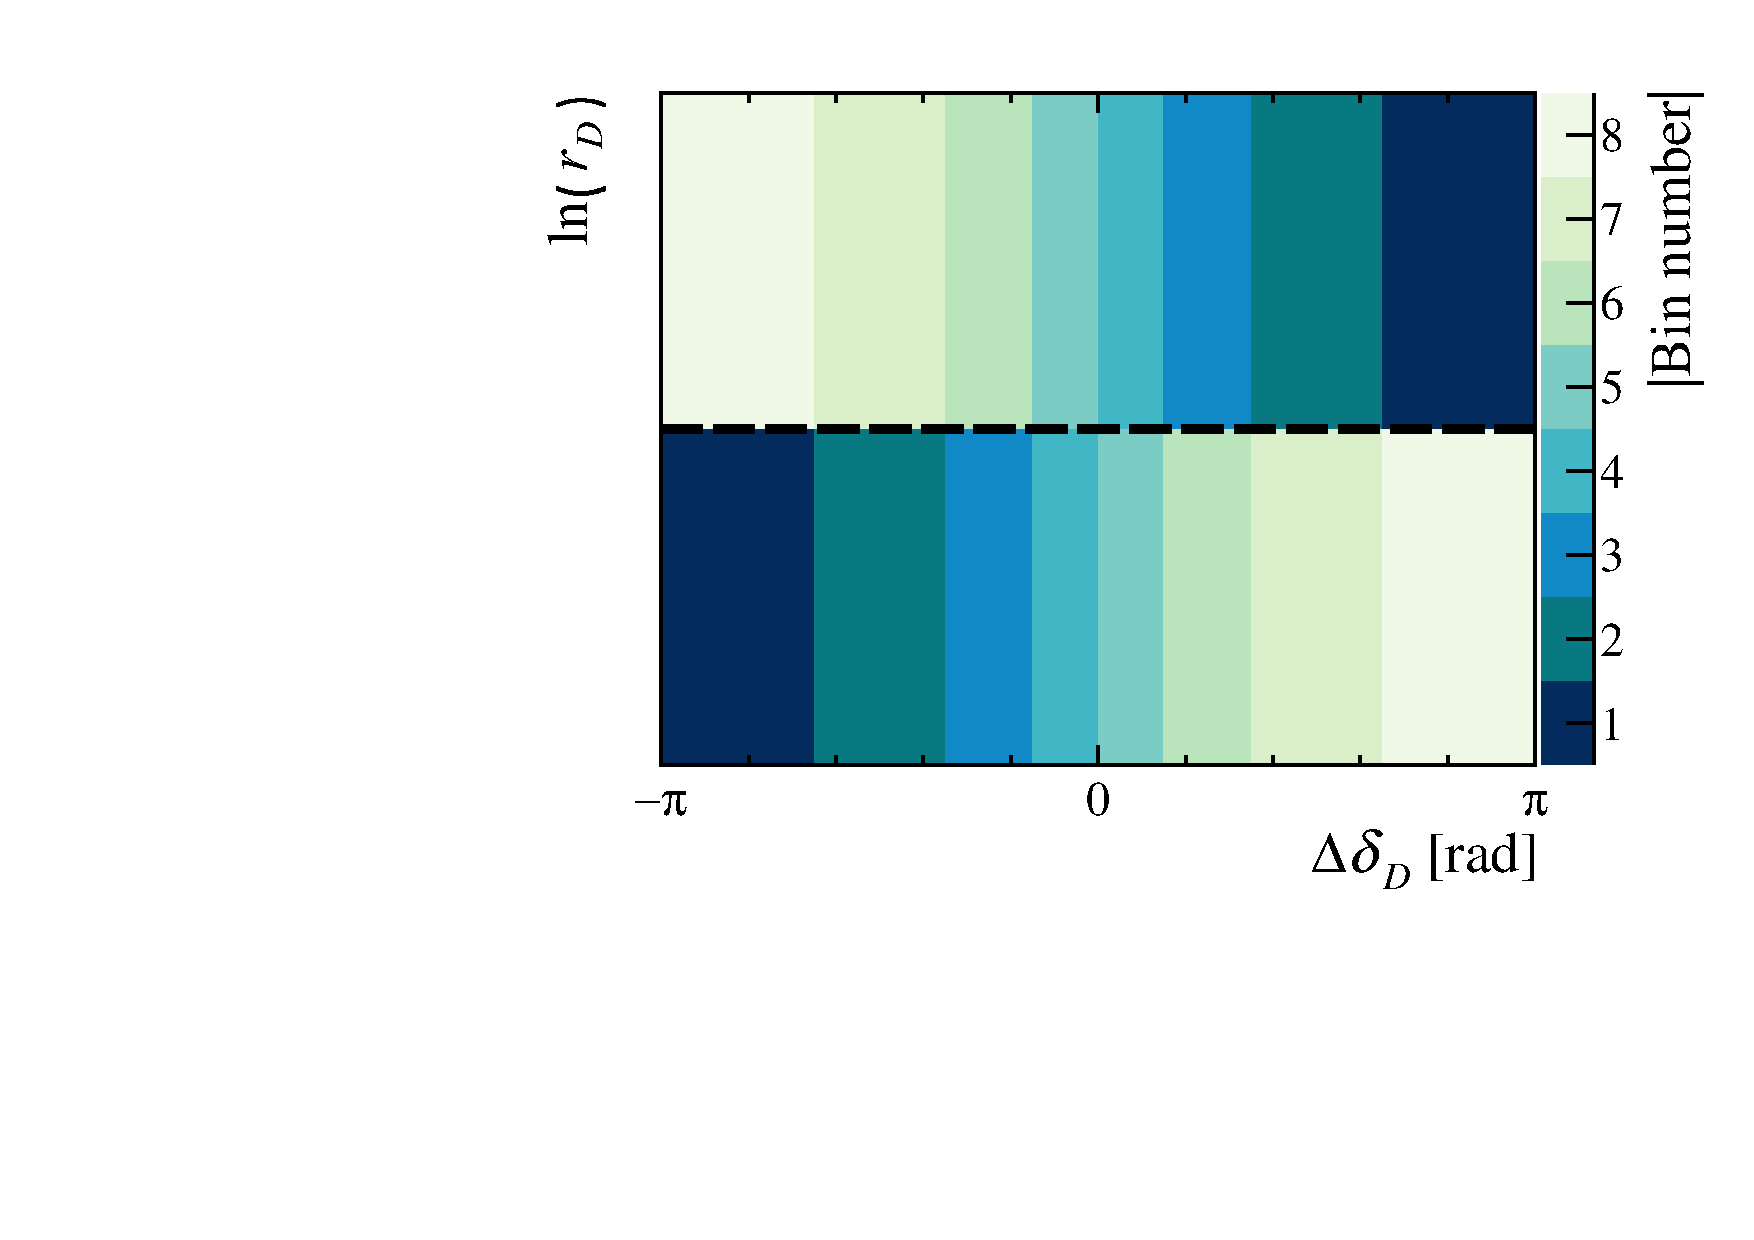
\includegraphics[height = 3.5cm]{Plots/BinningSchemePlot_8Bins.pdf}
      \vspace{-0.3cm}
      \caption*{8 bins}
    \end{subfigure}
    \caption*{$D^0\to K^+K^-\pi^+\pi^-$ binning scheme}
  \end{figure}
\end{frame}

\begin{frame}{Model-dependent measurement with $D\to K^+K^-\pi^+\pi^-$}
  \begin{center}
    \large From the phase-space binned asymmetries, we obtain:\\
    \vspace{0.2cm}
    $\gamma = (116^{+12}_{-14})^\circ$
  \end{center}
  \vspace{-0.2cm}
  \begin{figure}[htb]
    \centering
    \begin{subfigure}{0.5\textwidth}
      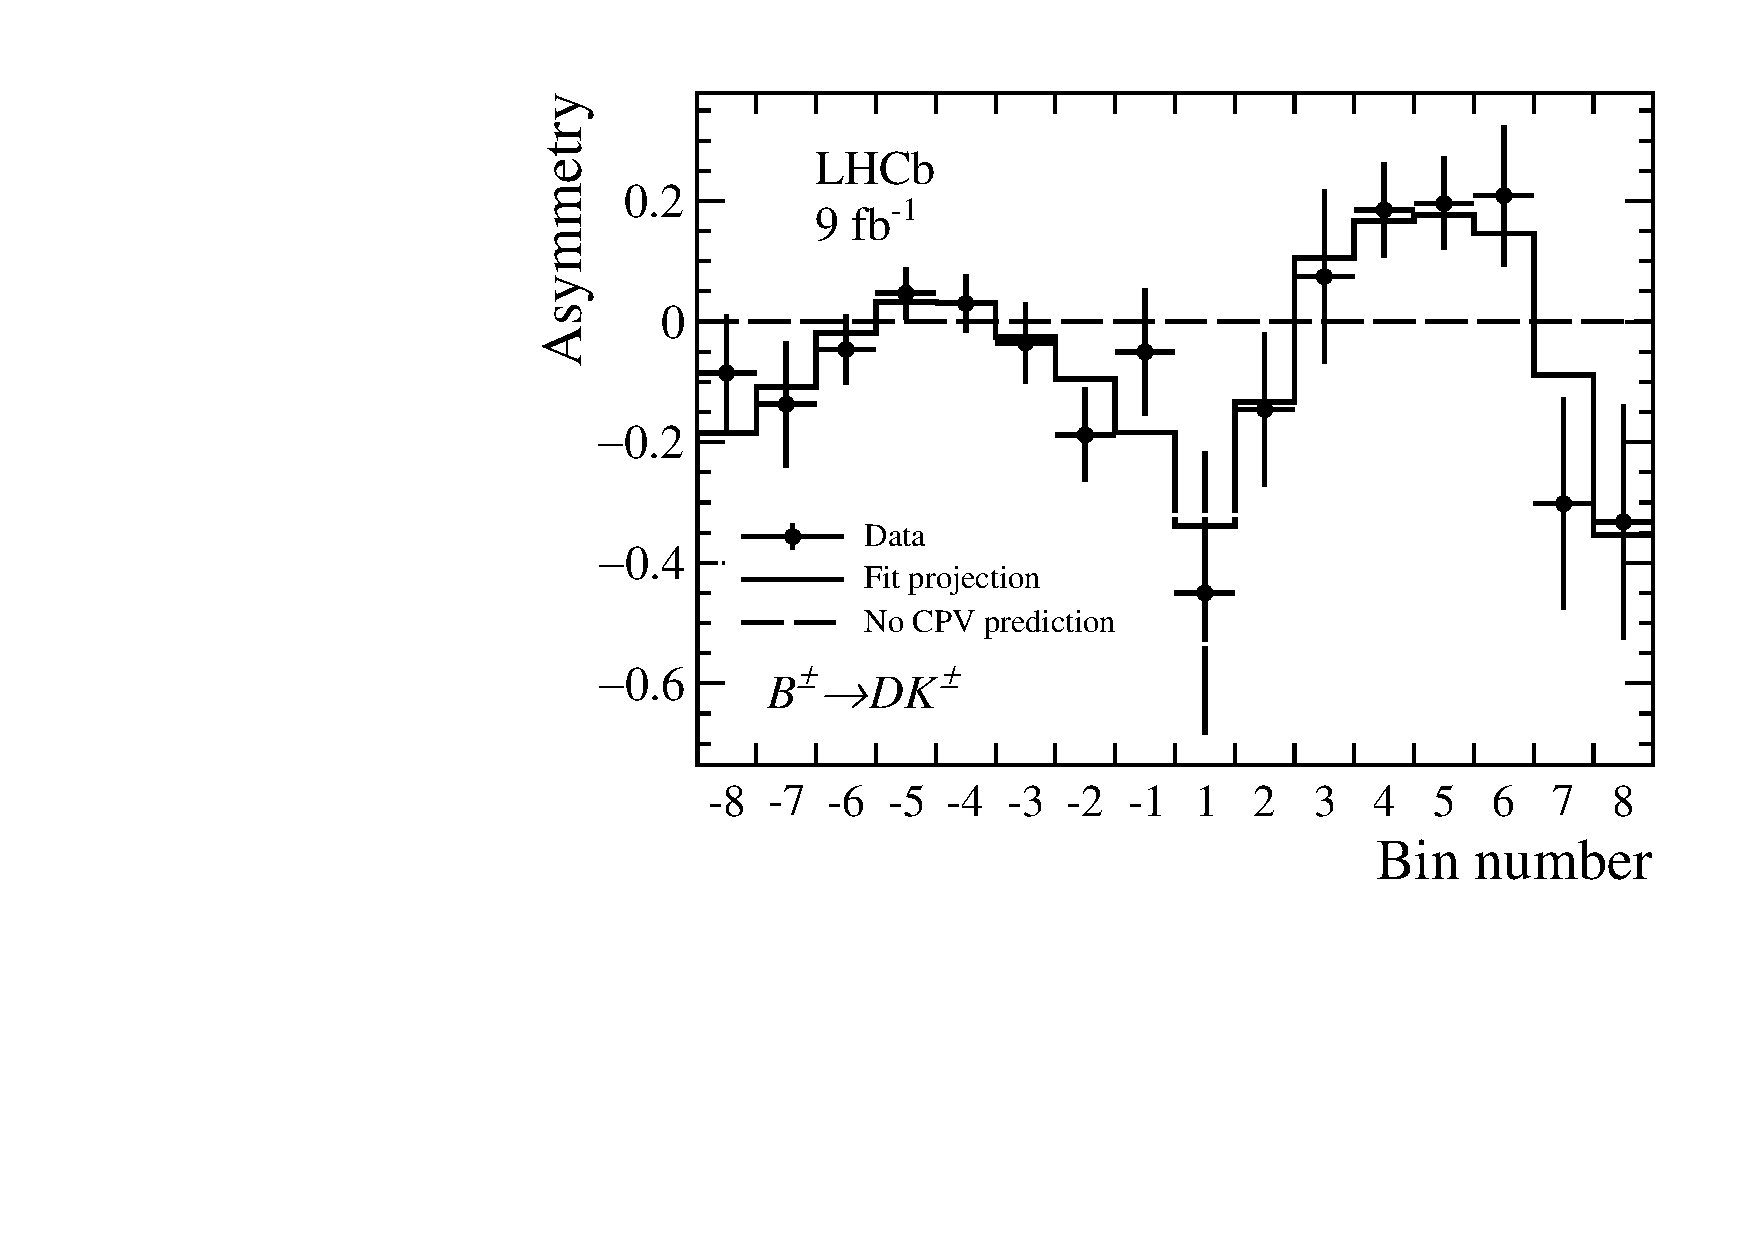
\includegraphics[width=1\textwidth]{Plots/BinAsymmetries_dk_ModelDependent.pdf}
    \end{subfigure}%
    \begin{subfigure}{0.5\textwidth}
      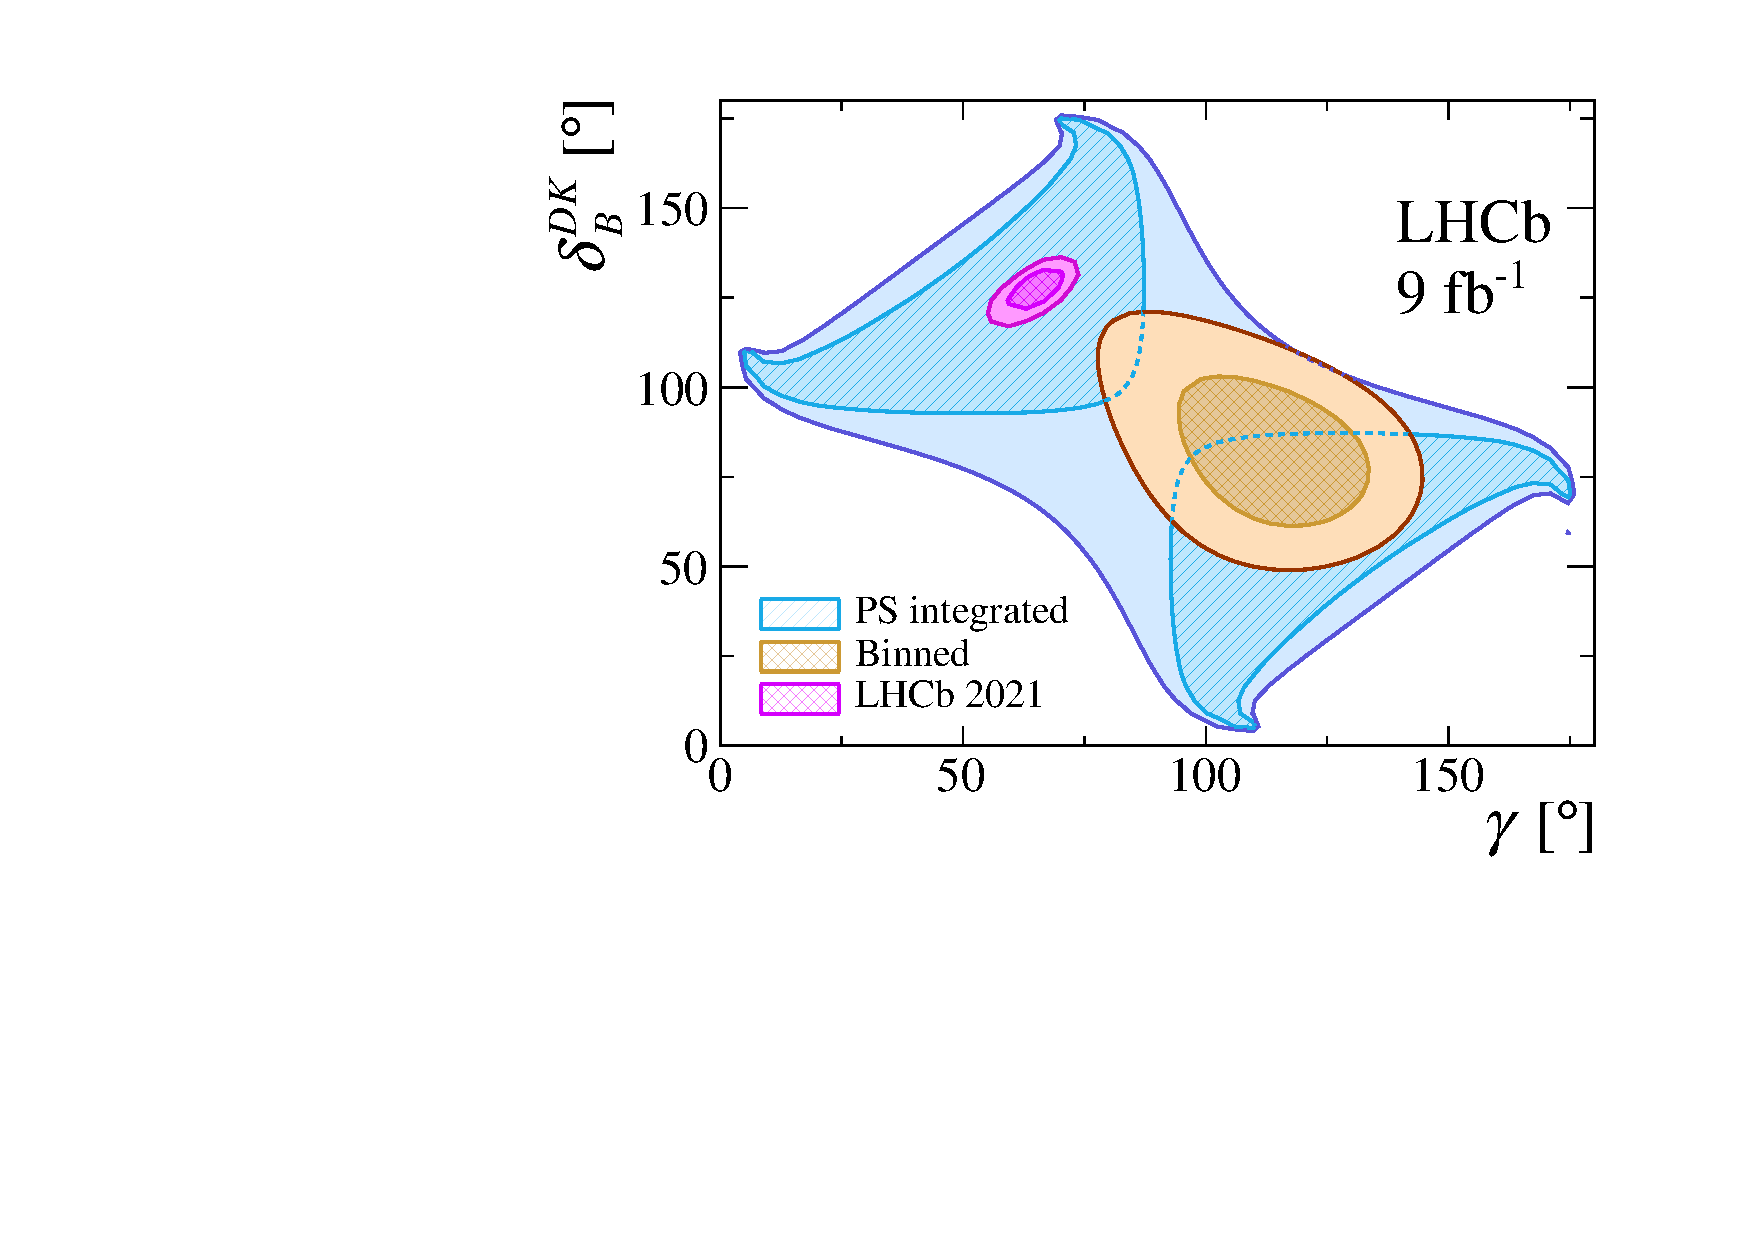
\includegraphics[width=1\textwidth]{Plots/gammacharm_lhcb_KKpipi_GLW_KKpipi_GGSZ_lhcb_2020_beauty_and_charm_g_d_dk_ModelDependent.pdf}
    \end{subfigure}
    \vspace{-0.5cm}
    \caption*{\tiny\href{https://link.springer.com/article/10.1140/epjc/s10052-023-11560-5}{Eur. Phys. J. C \textbf{83}, 547 (2023)}}
  \end{figure}
  \vspace{-0.5cm}
  \begin{center}
    {\large How will this evolve with model-independent BESIII inputs? Will the $3\sigma$ tension reduce?}
  \end{center}
\end{frame}

\begin{frame}{Motivation for this analysis}
  \begin{center}
    {\large What is new in this presentation?}
  \end{center}
  \begin{itemize}
    \setlength\itemsep{1.5em}
    \item{Analysis of $D\to K^+K^-\pi^+\pi^-$ and $D\to\pi^+\pi^-\pi^+\pi^-$ at BESIII has reached an advanced stage of review}
    \item{Update $K^+K^-\pi^+\pi^-$ result to obtain model-independent value of $\gamma$}
    \item{First binned measurement of $\gamma$ using $\pi^+\pi^-\pi^+\pi^-$}
    \item{Aim for a quick B2OC and RC review as the selection and global fit is identical to previous analysis}
  \end{itemize}
\end{frame}

\begin{frame}{Motivation for this analysis}
  \begin{center}
    {\color{blue}The results shown in this presentation make use of strong-phase results from the BESIII collaboration. They derive from mature analyses, but are not yet public, and remain preliminary in nature. They are not to be shown outside LHCb. We thank the BESIII management for the privilege of being allowed to use them during the review of this measurement.}
  \end{center}
\end{frame}

\section{Strong-phase inputs from BESIII}
\begin{frame}{$D^0\to K^+K^-\pi^+\pi^-$ strong-phase results}
  \begin{center}
    $D^0\to K^+K^-\pi^+\pi^-$ analysis uses the $2\times4$ binning scheme
  \end{center}
  \vspace{0.0cm}
  \begin{columns}
    \begin{column}{0.5\textwidth}
      \vspace{-0.5cm}
      \begin{align*}
        c_1 =& -0.28 \pm 0.09 \pm 0.01 \\
        s_1 =& -0.68 \pm 0.24 \pm 0.04 \\
        c_2 =& +0.83 \pm 0.04 \pm 0.01 \\
        s_2 =& -0.18 \pm 0.19 \pm 0.03 \\
        c_3 =& +0.83 \pm 0.03 \pm 0.01 \\
        s_3 =& +0.27 \pm 0.17 \pm 0.03 \\
        c_4 =& -0.28 \pm 0.10 \pm 0.01 \\
        s_4 =& +0.54 \pm 0.28 \pm 0.04
      \end{align*}
    \end{column}
    \begin{column}{0.5\textwidth}
      \begin{figure}
        \centering
        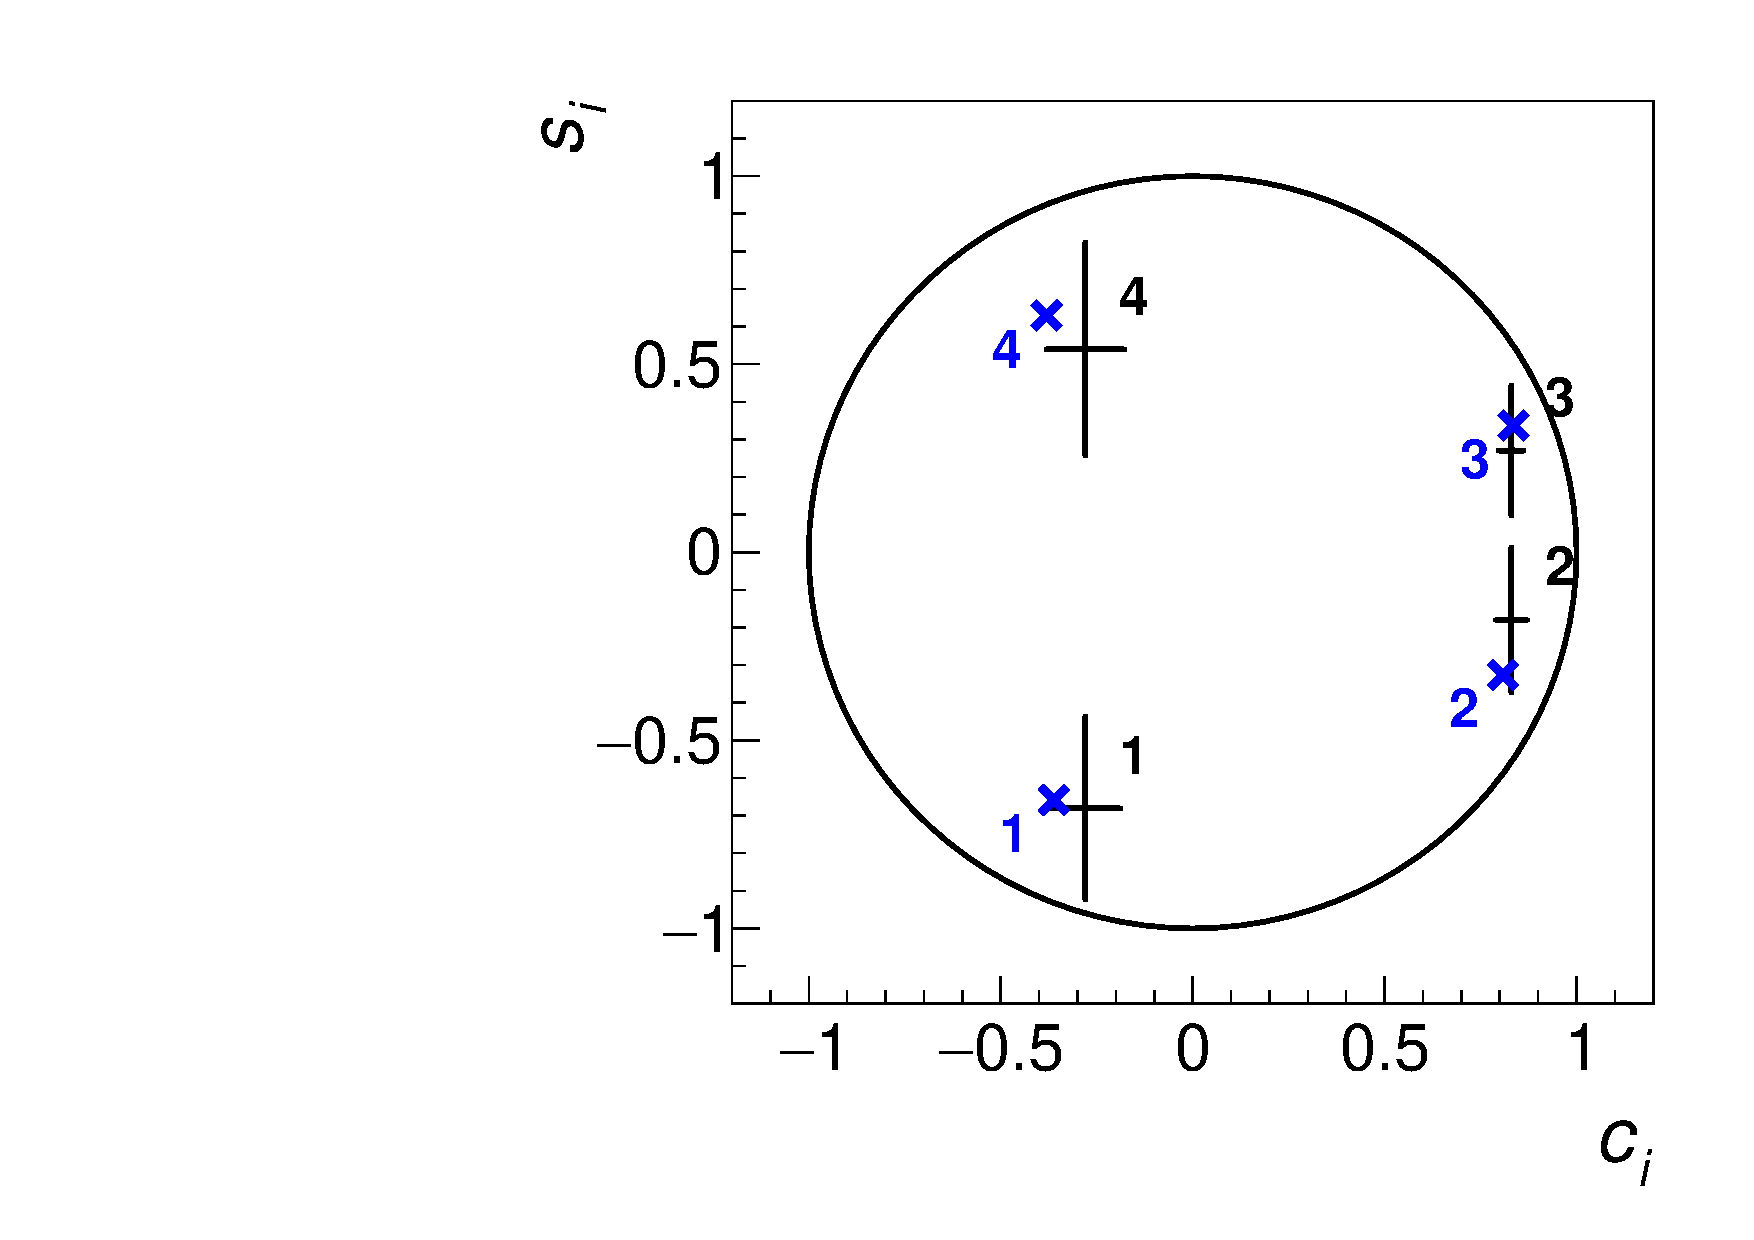
\includegraphics[width=1.0\textwidth]{Plots/cisi_FitResults_Model.pdf}
      \end{figure}
    \end{column}
  \end{columns}
  \begin{center}
    Measured values (black) are consistent with model predictions (blue)
  \end{center}
\end{frame}

\begin{frame}{$D^0\to K^+K^-\pi^+\pi^-$ strong-phase results}
  \begin{center}
    $D^0\to\pi^+\pi^-\pi^+\pi^-$ analysis uses the $2\times5$ ``optimal'' binning scheme
  \end{center}
  \vspace{0.0cm}
  \begin{columns}
    \begin{column}{0.5\textwidth}
      \vspace{-0.5cm}
      \begin{align*}
        c_1 =& +0.12 \pm 0.09 \pm 0.02 \\
        s_1 =& -0.42 \pm 0.21 \pm 0.04 \\
        c_2 =& +0.74 \pm 0.04 \pm 0.02 \\
        s_2 =& -0.39 \pm 0.16 \pm 0.06 \\
        c_3 =& +0.81 \pm 0.03 \pm 0.01 \\
        s_3 =& -0.25 \pm 0.12 \pm 0.03 \\
        c_4 =& +0.42 \pm 0.06 \pm 0.02 \\
        s_4 =& +0.86 \pm 0.19 \pm 0.07 \\
        c_5 =& -0.27 \pm 0.09 \pm 0.03 \\
        s_5 =& -0.22 \pm 0.25 \pm 0.08
      \end{align*}
    \end{column}
    \begin{column}{0.5\textwidth}
      \begin{figure}
        \centering
        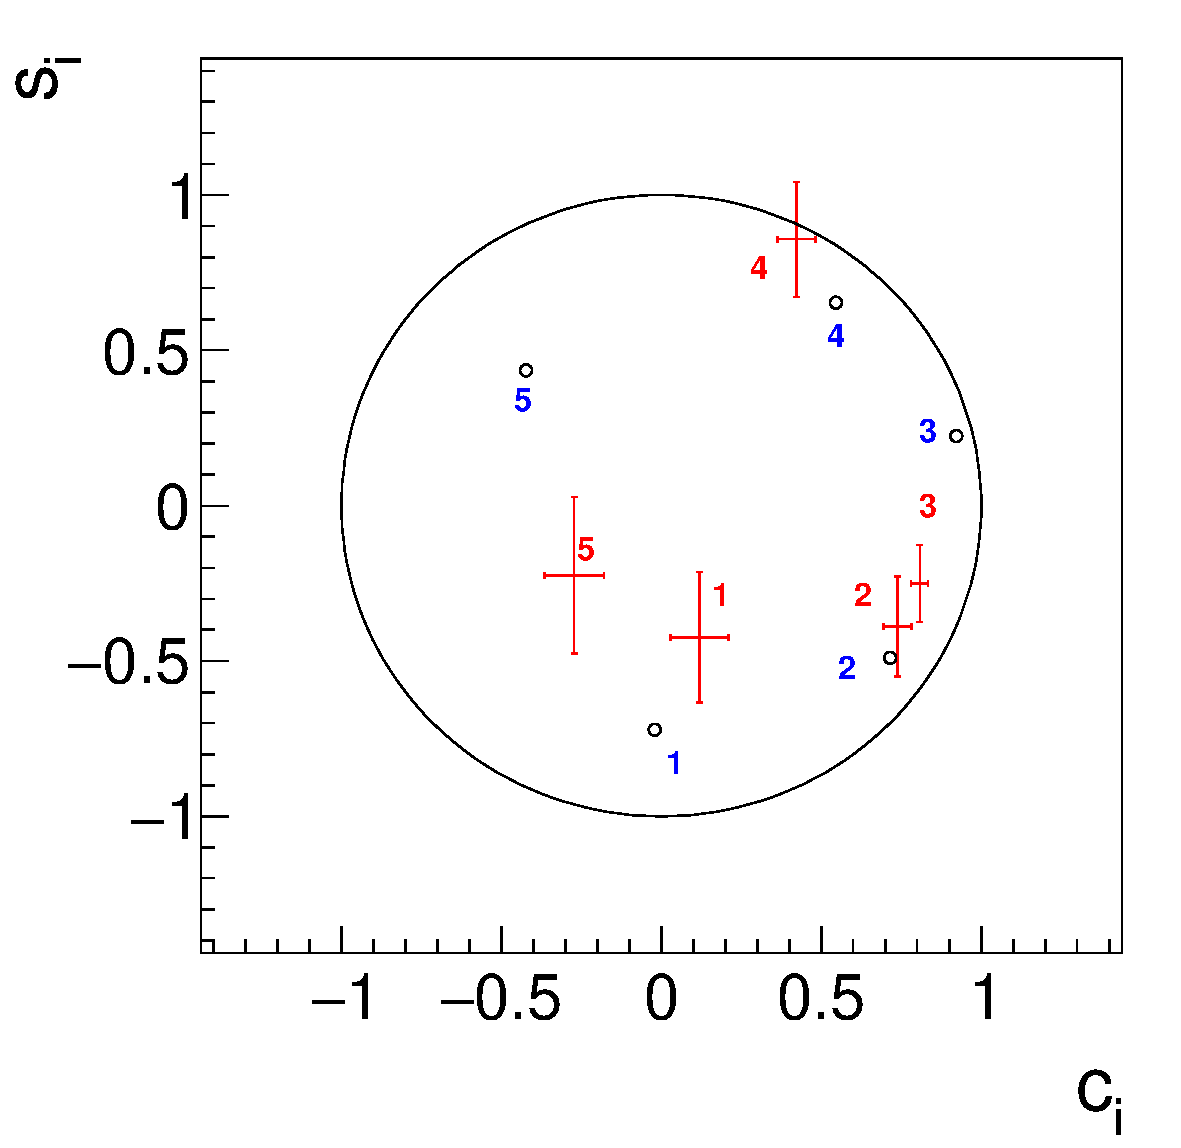
\includegraphics[width=1.0\textwidth]{Plots/CiSiOptim.pdf}
      \end{figure}
    \end{column}
  \end{columns}
  \begin{center}
    The HyperPlot software is used (binary lookup tree in 5D phase space)
  \end{center}
\end{frame}

\section{Global fit}
\begin{frame}{Global fit}
  \begin{center}
    {\large Global fit of $K^+K^-\pi^+\pi^-$ mode remains the same:}
  \end{center}
  \begin{figure}
    \centering
    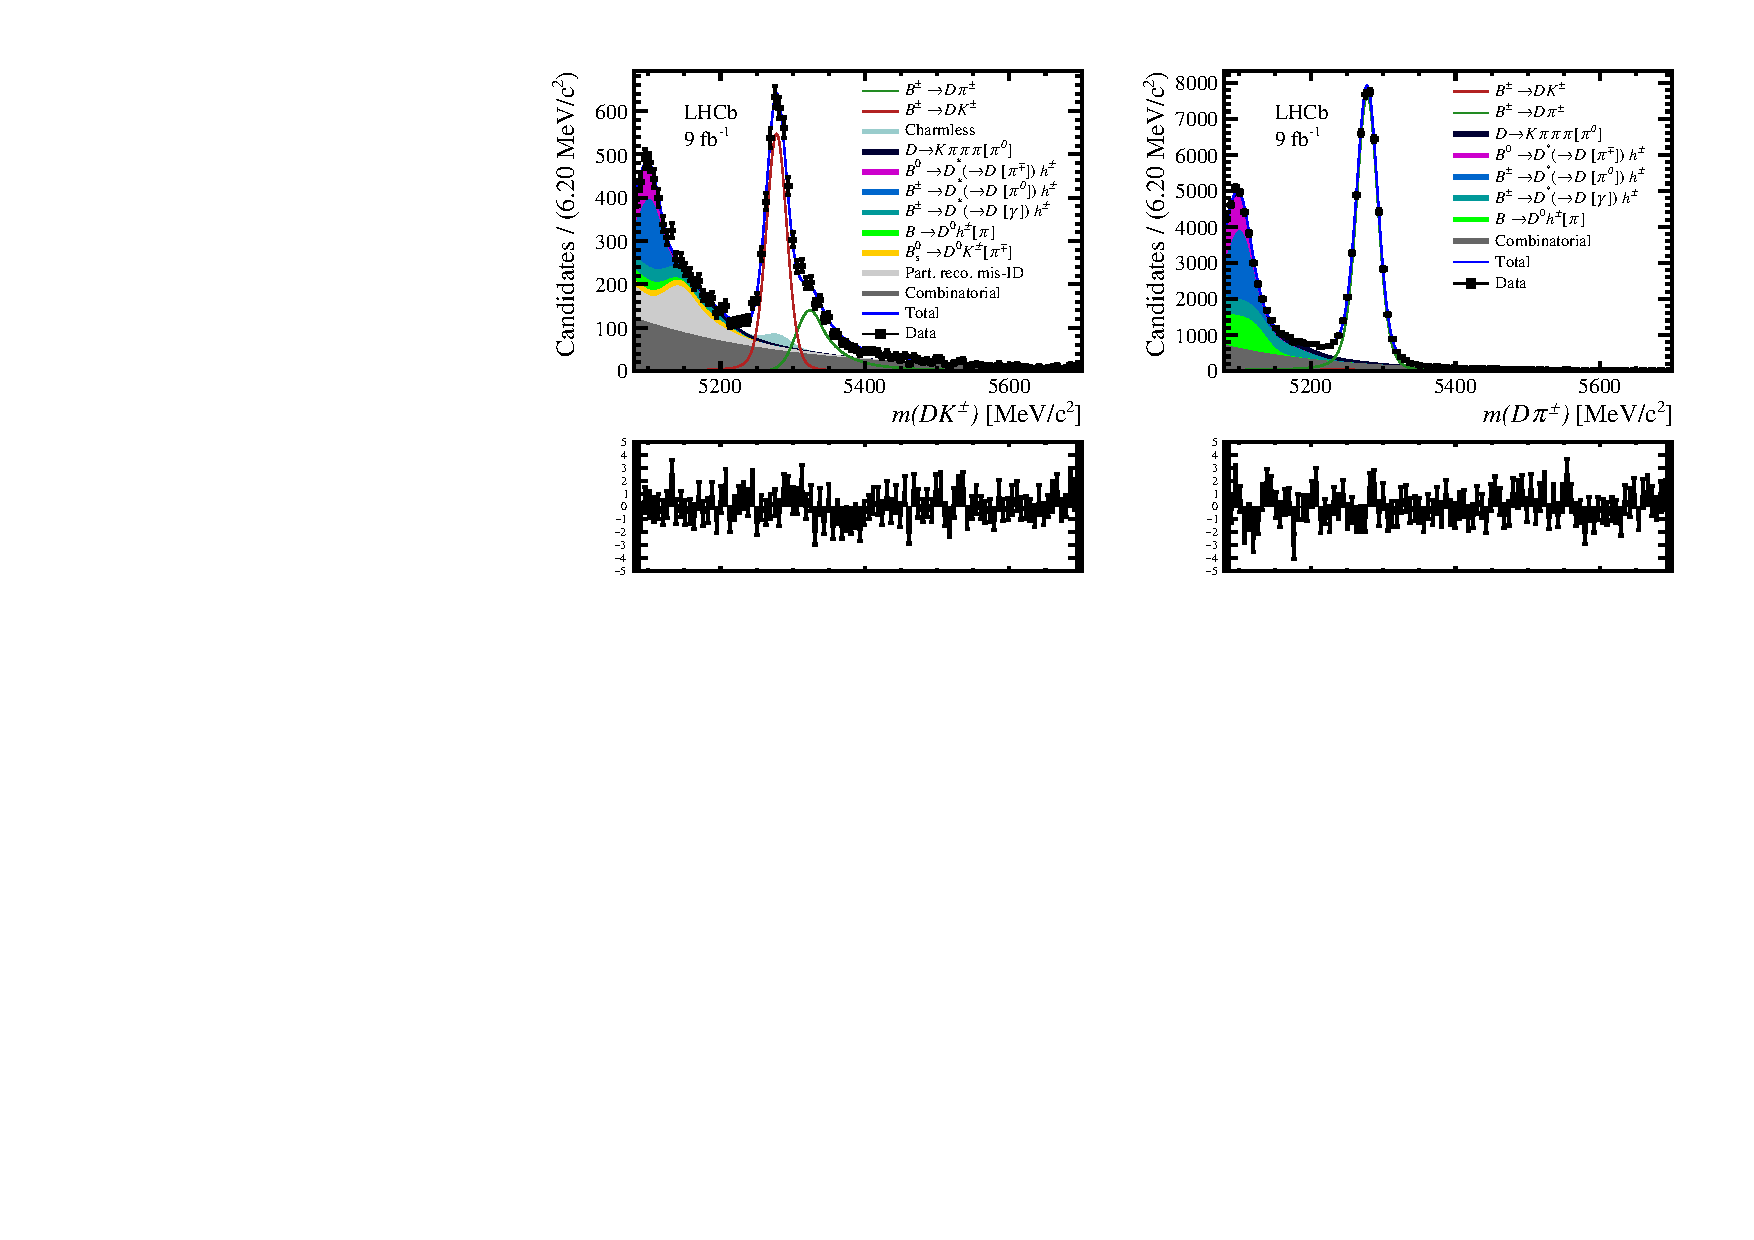
\includegraphics[width = 0.9\textwidth,trim={0 0 0 0},clip=true]{Plots/d2kkpipi_fiveL_allDP.pdf}
  \end{figure}
  \vspace{-0.5cm}
  \begin{itemize}
    \item{$B^\pm\to[K^+K^-\pi^+\pi^-]_Dh^\pm$ signal yield:}
    \begin{itemize}
      \item{$B^\pm\to DK^\pm$: $3051 \pm 38$}
      \item{$B^\pm\to D\pi^\pm$: $44356 \pm 218$}
    \end{itemize}
  \end{itemize}
\end{frame}

\begin{frame}{Global fit}
  \begin{center}
    {\large Global fit of $\pi^+\pi^-\pi^+\pi^-$ is included is a simultaneous fit:}
  \end{center}
  \begin{figure}
    \centering
    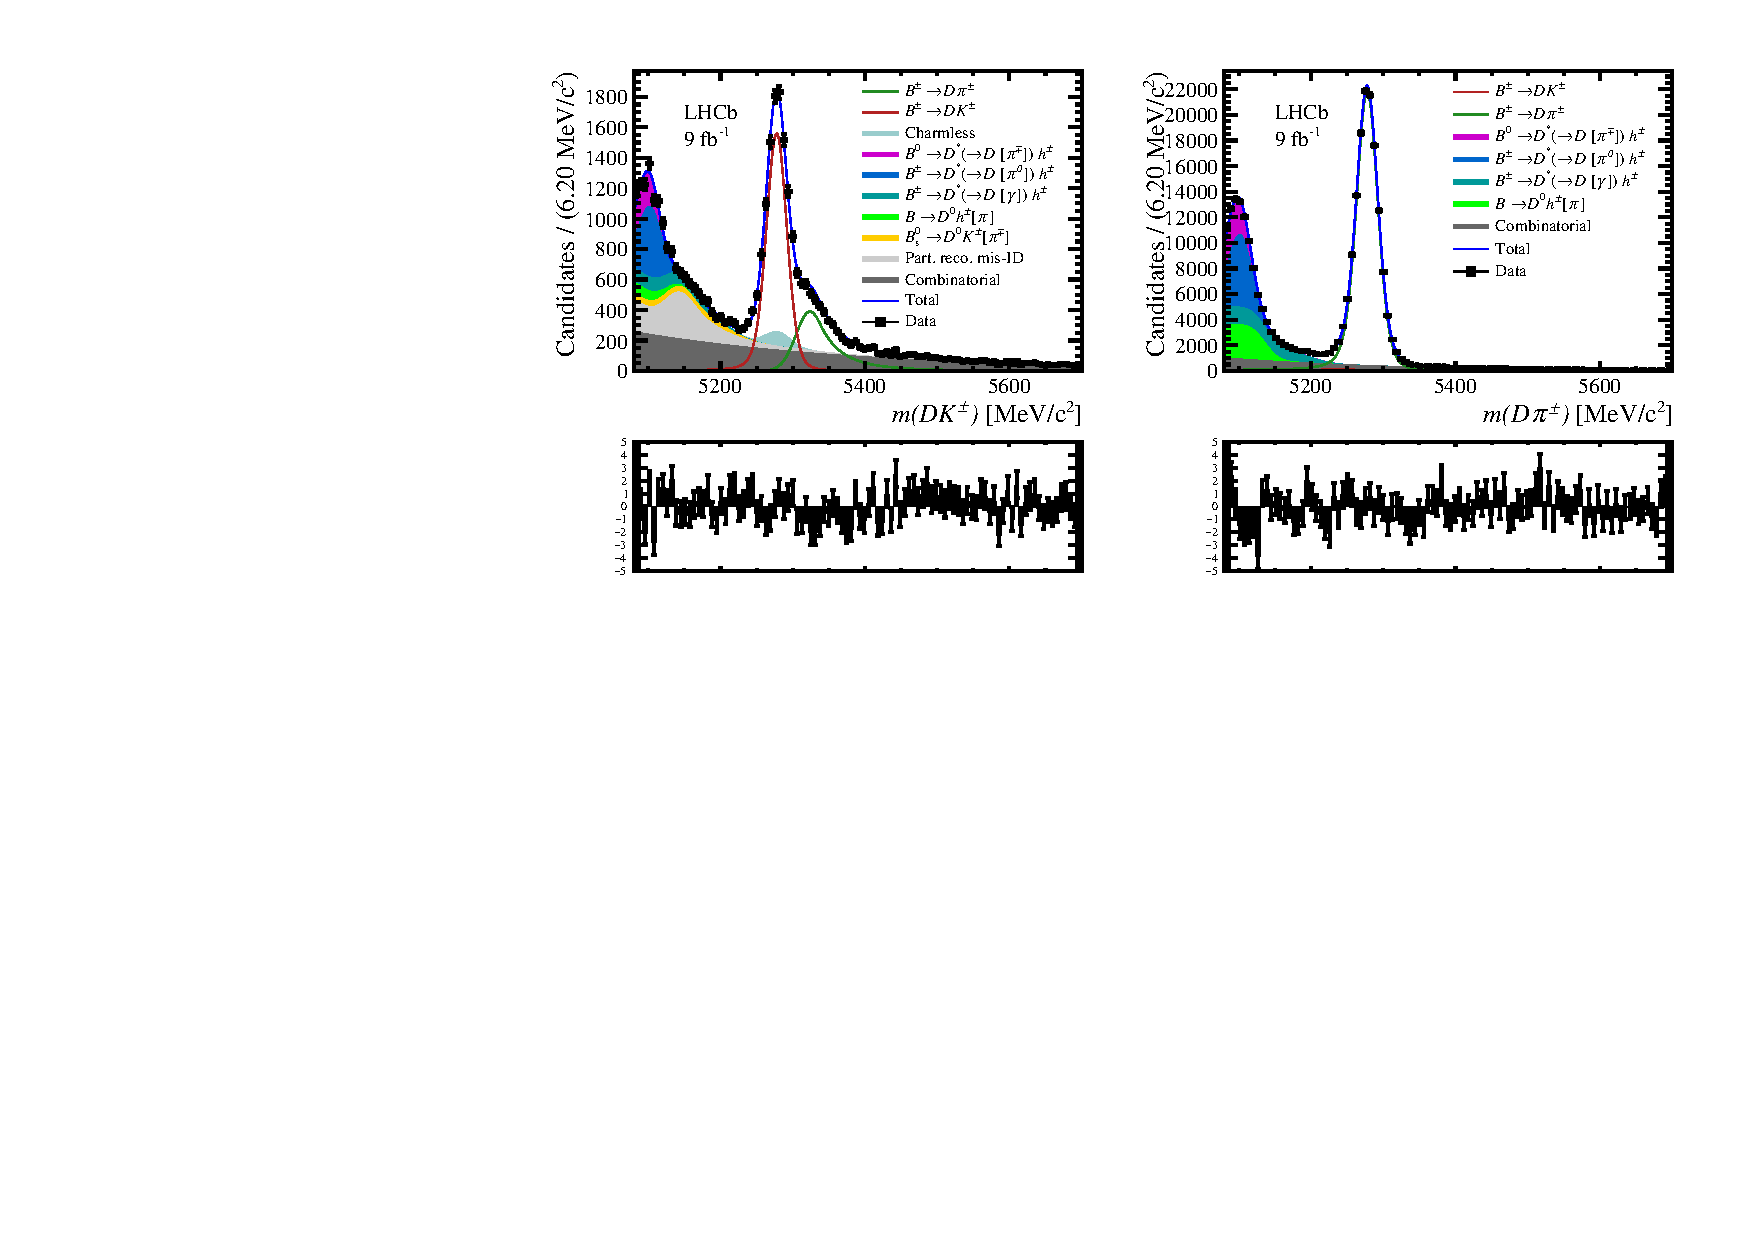
\includegraphics[width = 0.9\textwidth,trim={0 0 0 0},clip=true]{Plots/d2pipipipi_fiveL_allDP.pdf}
  \end{figure}
  \vspace{-0.5cm}
  \begin{itemize}
    \item{$B^\pm\to[\pi^+\pi^-\pi^+\pi^-]_Dh^\pm$ signal yield:}
    \begin{itemize}
      \item{$B^\pm\to DK^\pm$: $8745 \pm 105$}
      \item{$B^\pm\to D\pi^\pm$: $126314 \pm 385$}
    \end{itemize}
  \end{itemize}
\end{frame}

\section{CP fit}
\begin{frame}{CP fit}
  \begin{center}
    {\large After global fit, perform a ``CP fit'' to study CP violation:}
  \end{center}
  \begin{itemize}
    \setlength\itemsep{1.0em}
    \item{Split candidates by:}
    \begin{enumerate}
      \item{$B^+$ and $B^-$ charges}
      \item{$B^\pm\to DK^\pm$ and $B^\pm\to D\pi^\pm$ decays}
      \item{$D$ phase-space bins}
    \end{enumerate}
    \item{Combinatorial and low-mass backgrounds are floating in each category}
    \item{Parameterise signal yields in terms of $x_\pm^{DK}$, $y_\pm^{DK}$, $x_\xi^{D\pi}$, $y_\xi^{D\pi}$}
    \item{$2N - 1$ floating $F_i$ parameters}
    \item{\underline{$c_i$ and $s_i$ are Gaussian constrained}}
  \end{itemize}
\end{frame}

\begin{frame}{CP fit categories}
  \begin{center}
    {\large Summary of free parameters in the CP fit:}
  \end{center}
  \vspace{-0.5cm}
  \begin{columns}
    \begin{column}{0.5\textwidth}
      \begin{center}
        $K^+K^-\pi^+\pi^-$ \\
        $2\times2\times2\times4 = 32$ categories
      \end{center}
      \begin{itemize}
        \setlength\itemsep{0.0em}
        \item{6 CP observables}
        \item{7 $F_i$ parameters}
        \item{8 $c_i$ and $s_i$ parameters}
        \item{32 combinatorial yields}
        \item{32 low mass yields}
        \item{4 global normalisations}
        \item{Total: 89 parameters}
      \end{itemize}
    \end{column}
    \begin{column}{0.5\textwidth}
      \begin{center}
        $\pi^+\pi^-\pi^+\pi^-$ \\
        $2\times2\times2\times5 = 40$ categories
      \end{center}
      \begin{itemize}
        \setlength\itemsep{0.0em}
        \item{6 CP observables}
        \item{9 $F_i$ parameters}
        \item{10 $c_i$ and $s_i$ parameters}
        \item{40 combinatorial yields}
        \item{40 low mass yields}
        \item{4 global normalisations}
        \item{Total: 109 parameters}
      \end{itemize}
    \end{column}
  \end{columns}
  \vspace{0.3cm}
  \begin{center}
    In a combined fit where CP observables are shared, there are $89 + 109 - 6 = 192$ parameters
  \end{center}
\end{frame}

\begin{frame}{CP fit toy studies}
  \begin{center}
    In toy studies biases in $D\pi$ observables are consistent with model-dependent analysis
  \end{center}
  \begin{figure}
    \centering
    \begin{subfigure}{0.5\textwidth}
      \centering
      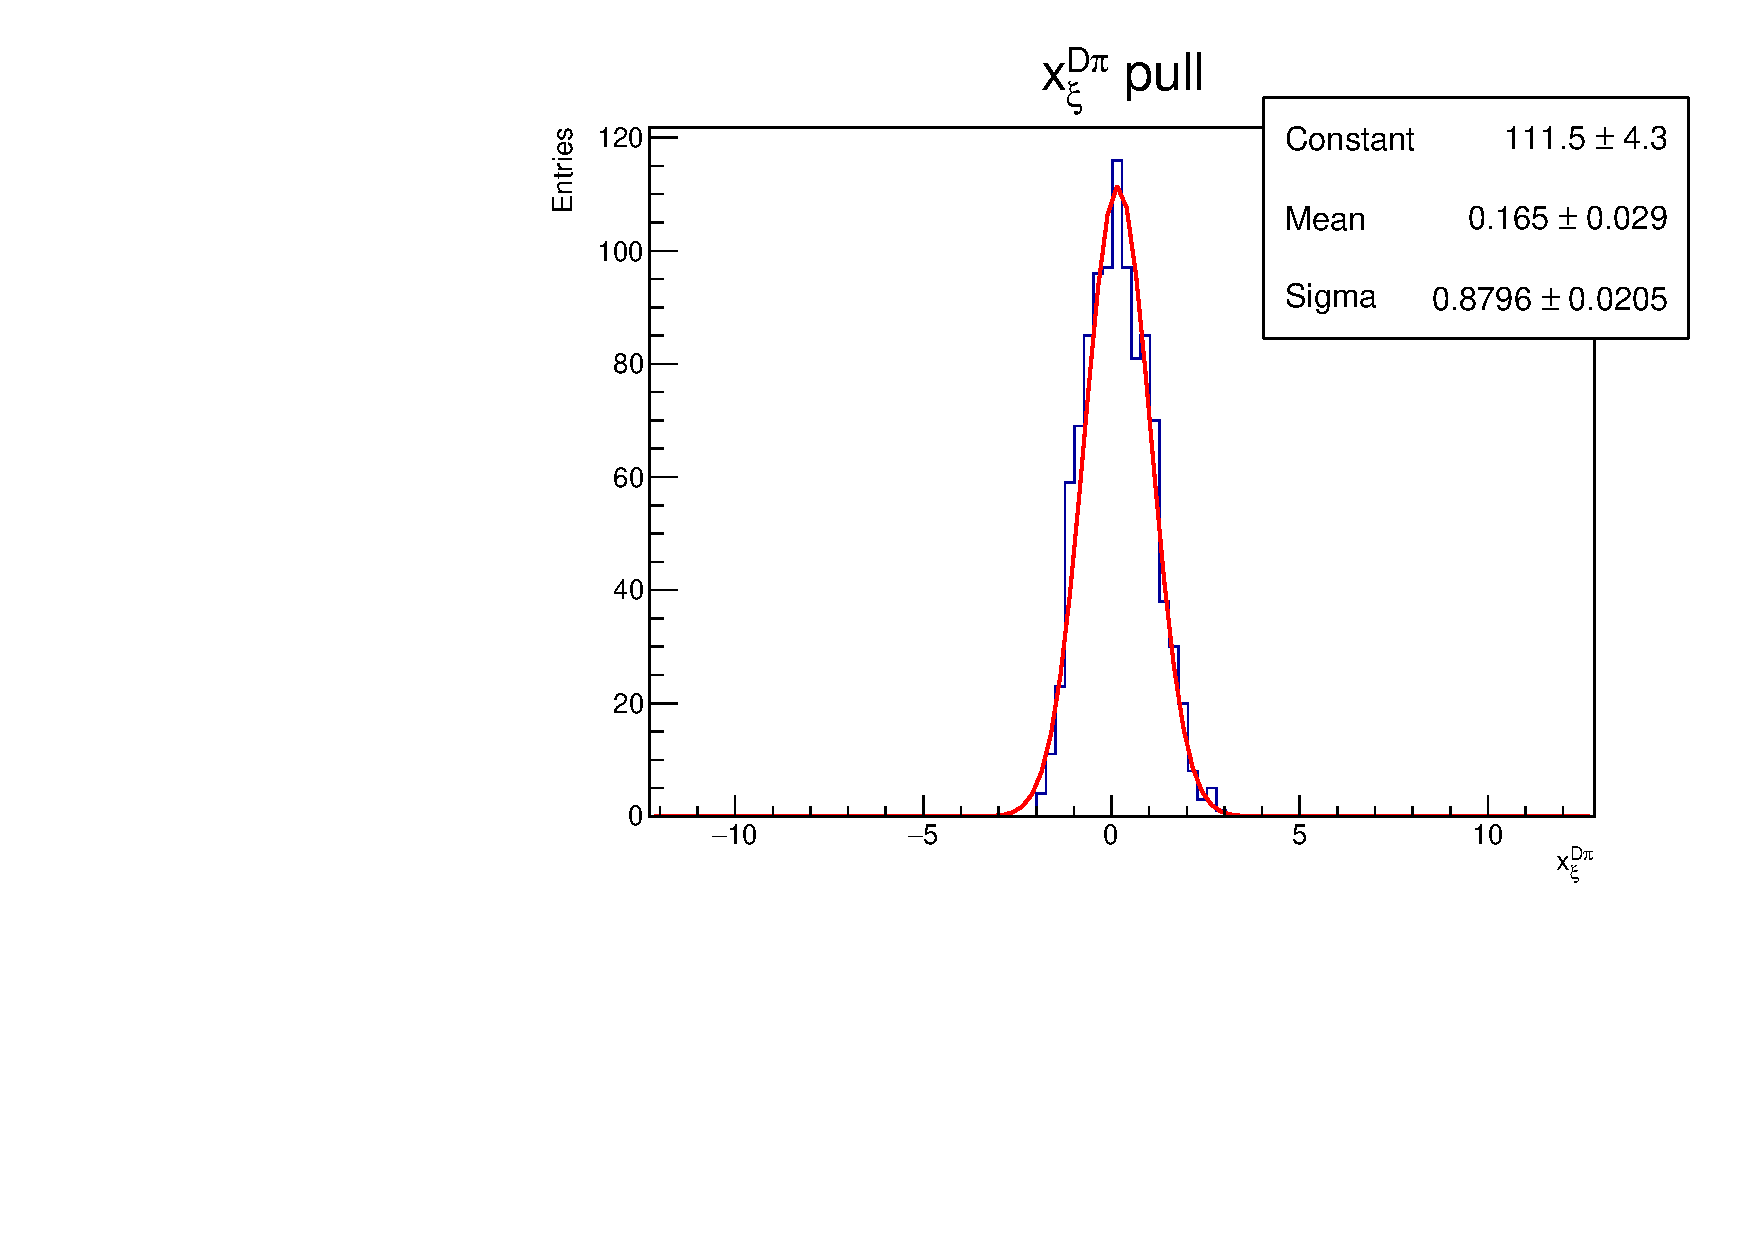
\includegraphics[width=1.0\textwidth]{Plots/A_Re_xi_dpi_pull.pdf}
      \vspace{-0.3cm}
      \caption*{$x_\xi^{D\pi}$}
    \end{subfigure}%
    \begin{subfigure}{0.5\textwidth}
      \centering
      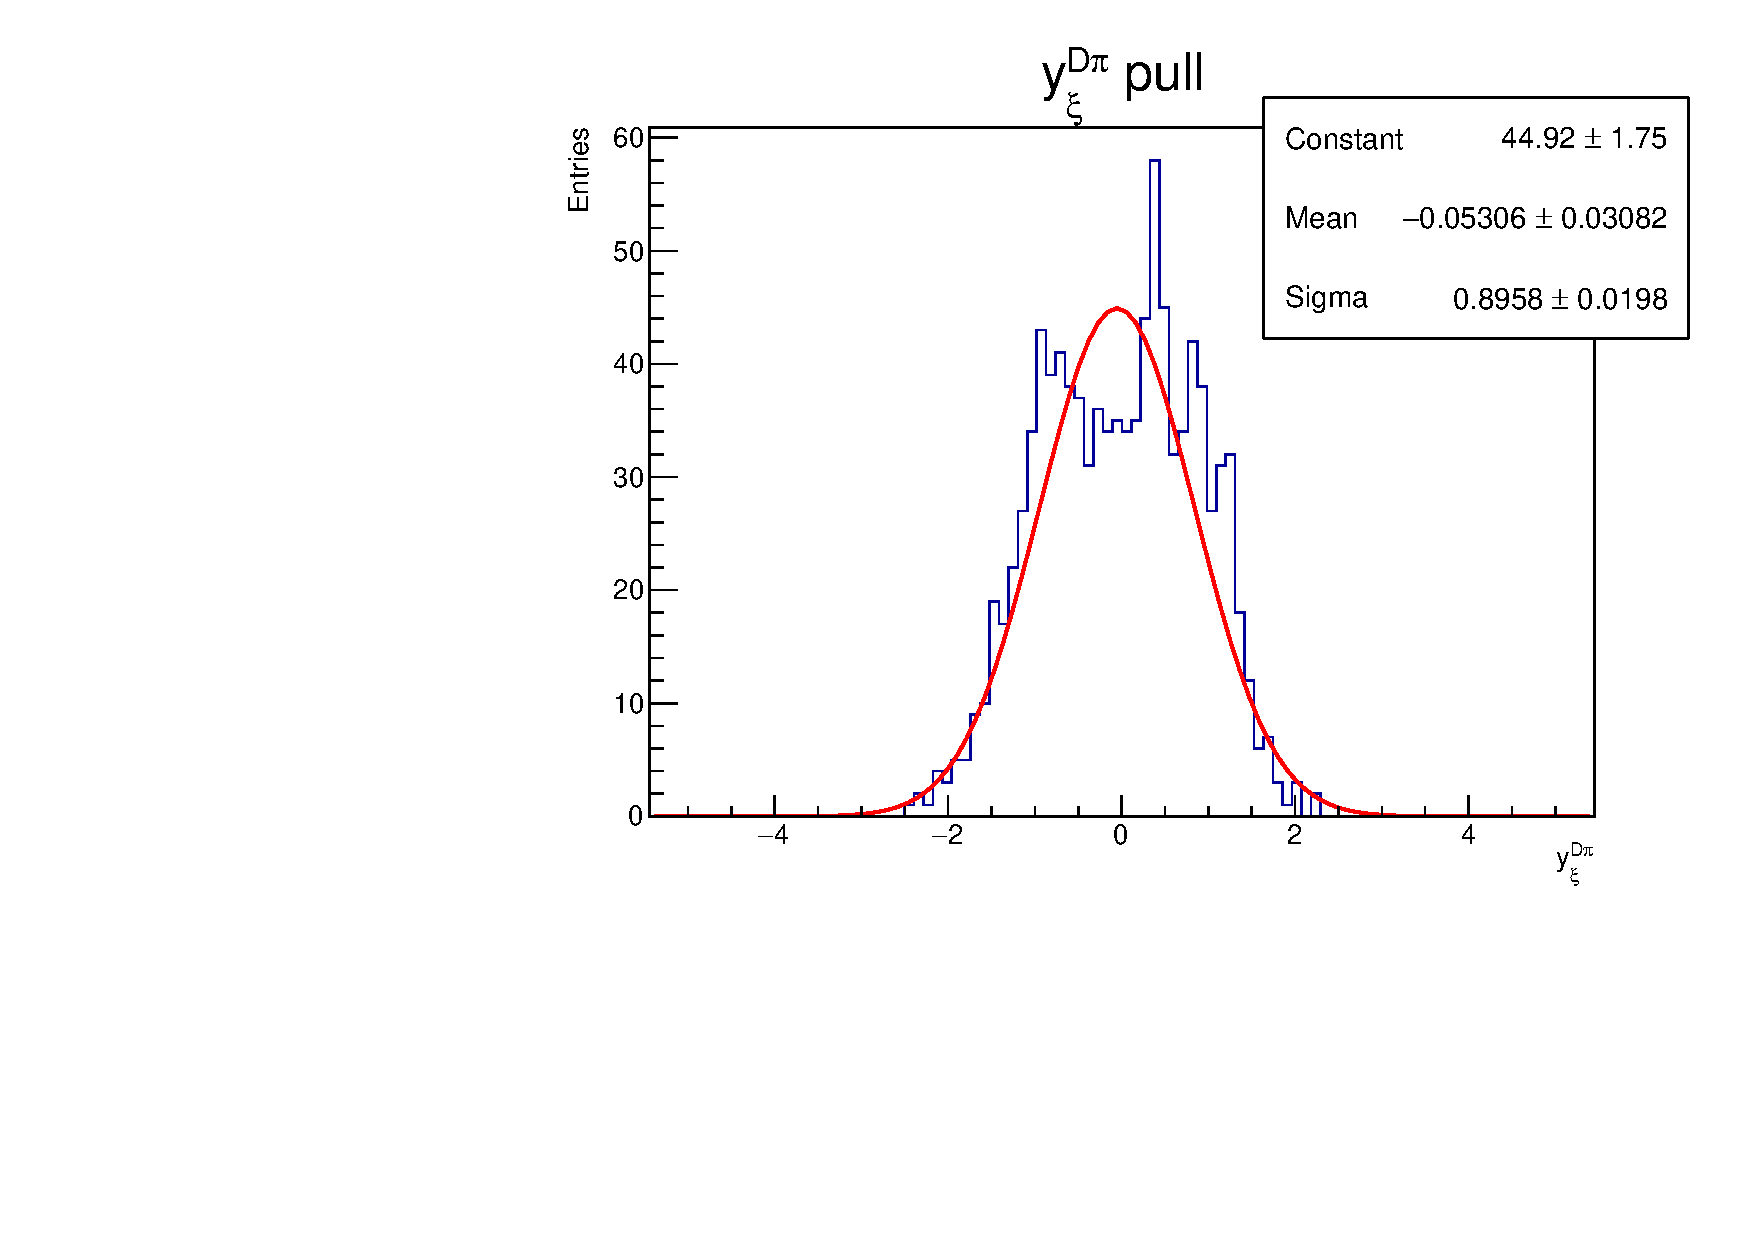
\includegraphics[width=1.0\textwidth]{Plots/A_Im_xi_dpi_pull.pdf}
      \vspace{-0.3cm}
      \caption*{$y_\xi^{D\pi}$}
    \end{subfigure}
    \caption*{$D^0\to K^+K^-\pi^+\pi^-$}
  \end{figure}
\end{frame}

\begin{frame}{CP fit toy studies}
  \begin{center}
    Minor biases in $x_\pm^{DK}$ are seen but can be corrected for...
  \end{center}
  \begin{figure}
    \centering
    \begin{subfigure}{0.5\textwidth}
      \centering
      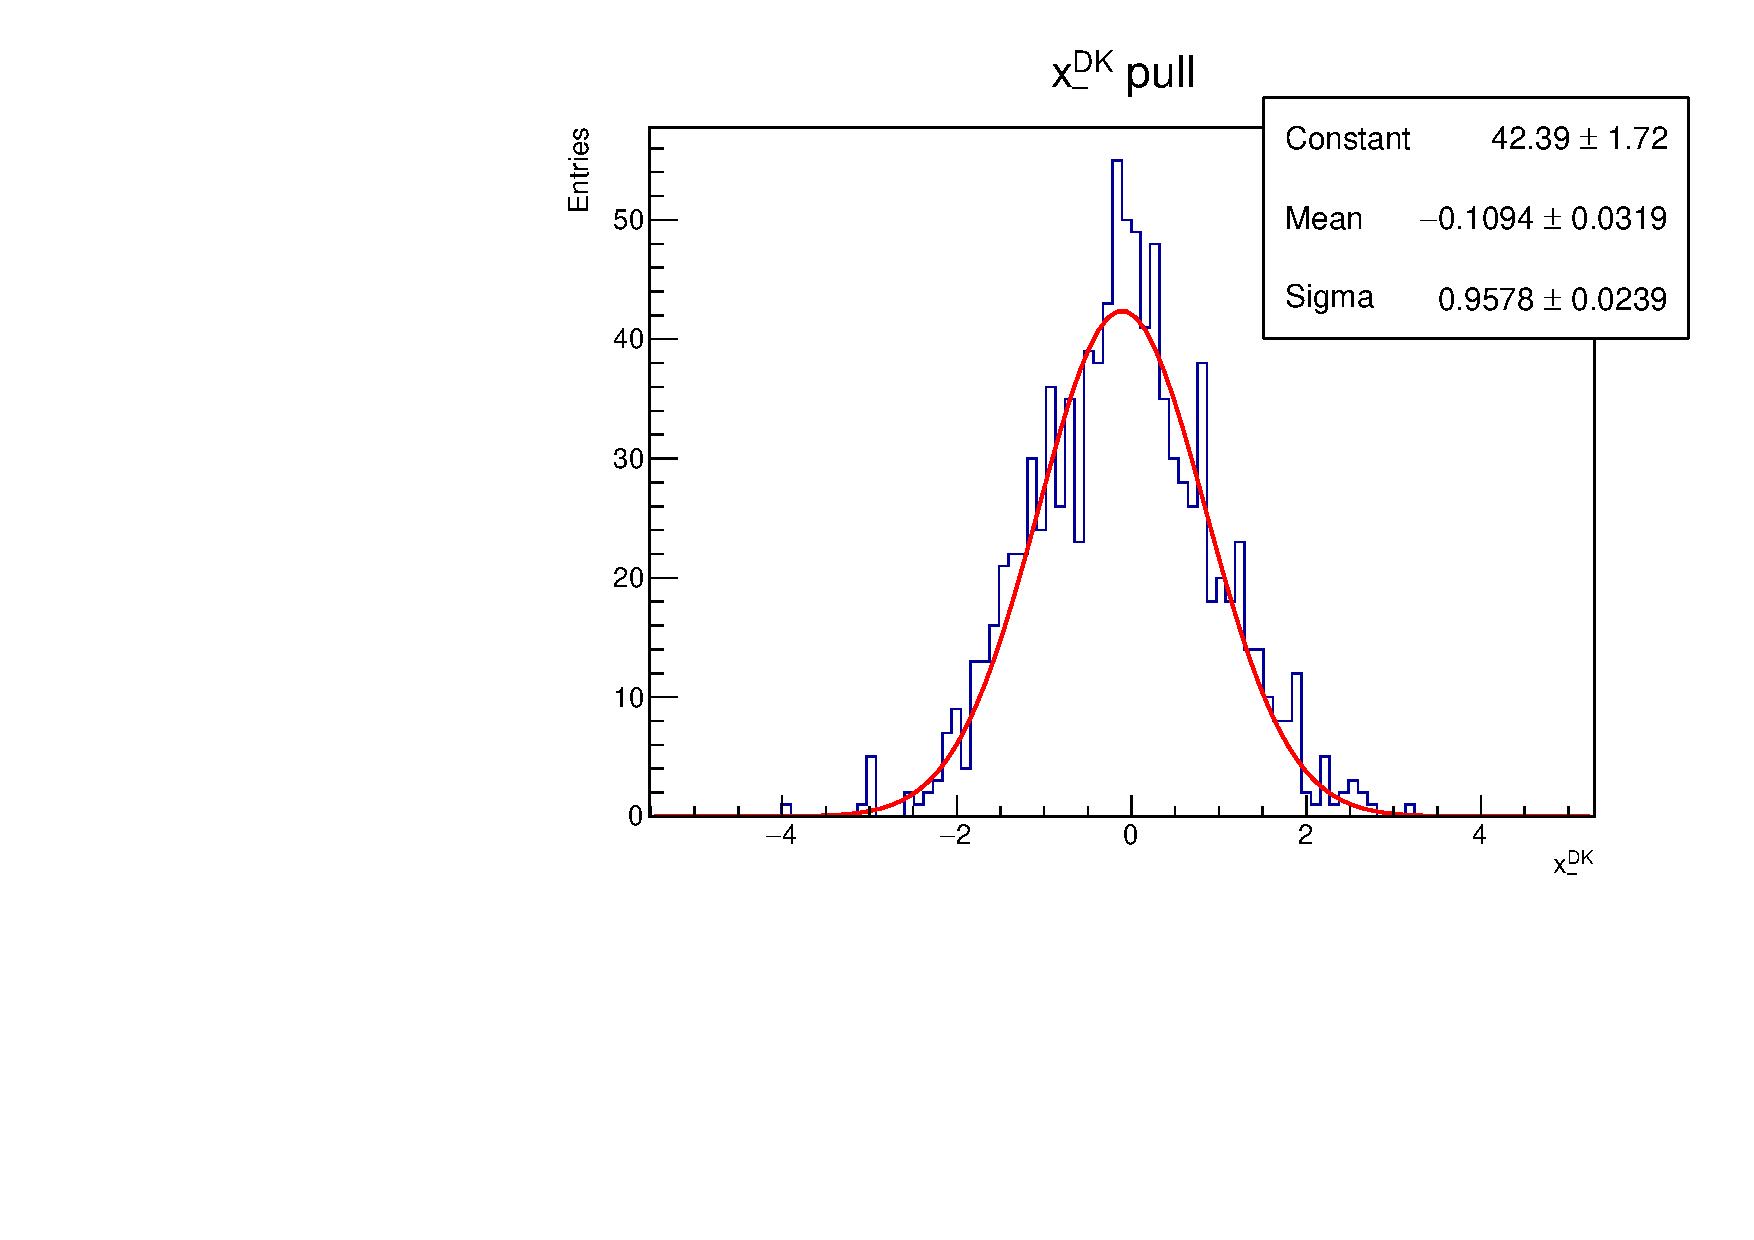
\includegraphics[width=1.0\textwidth]{Plots/A_xm_dk_pull.pdf}
      \vspace{-0.3cm}
      \caption*{$x_-^{DK}$}
    \end{subfigure}%
    \begin{subfigure}{0.5\textwidth}
      \centering
      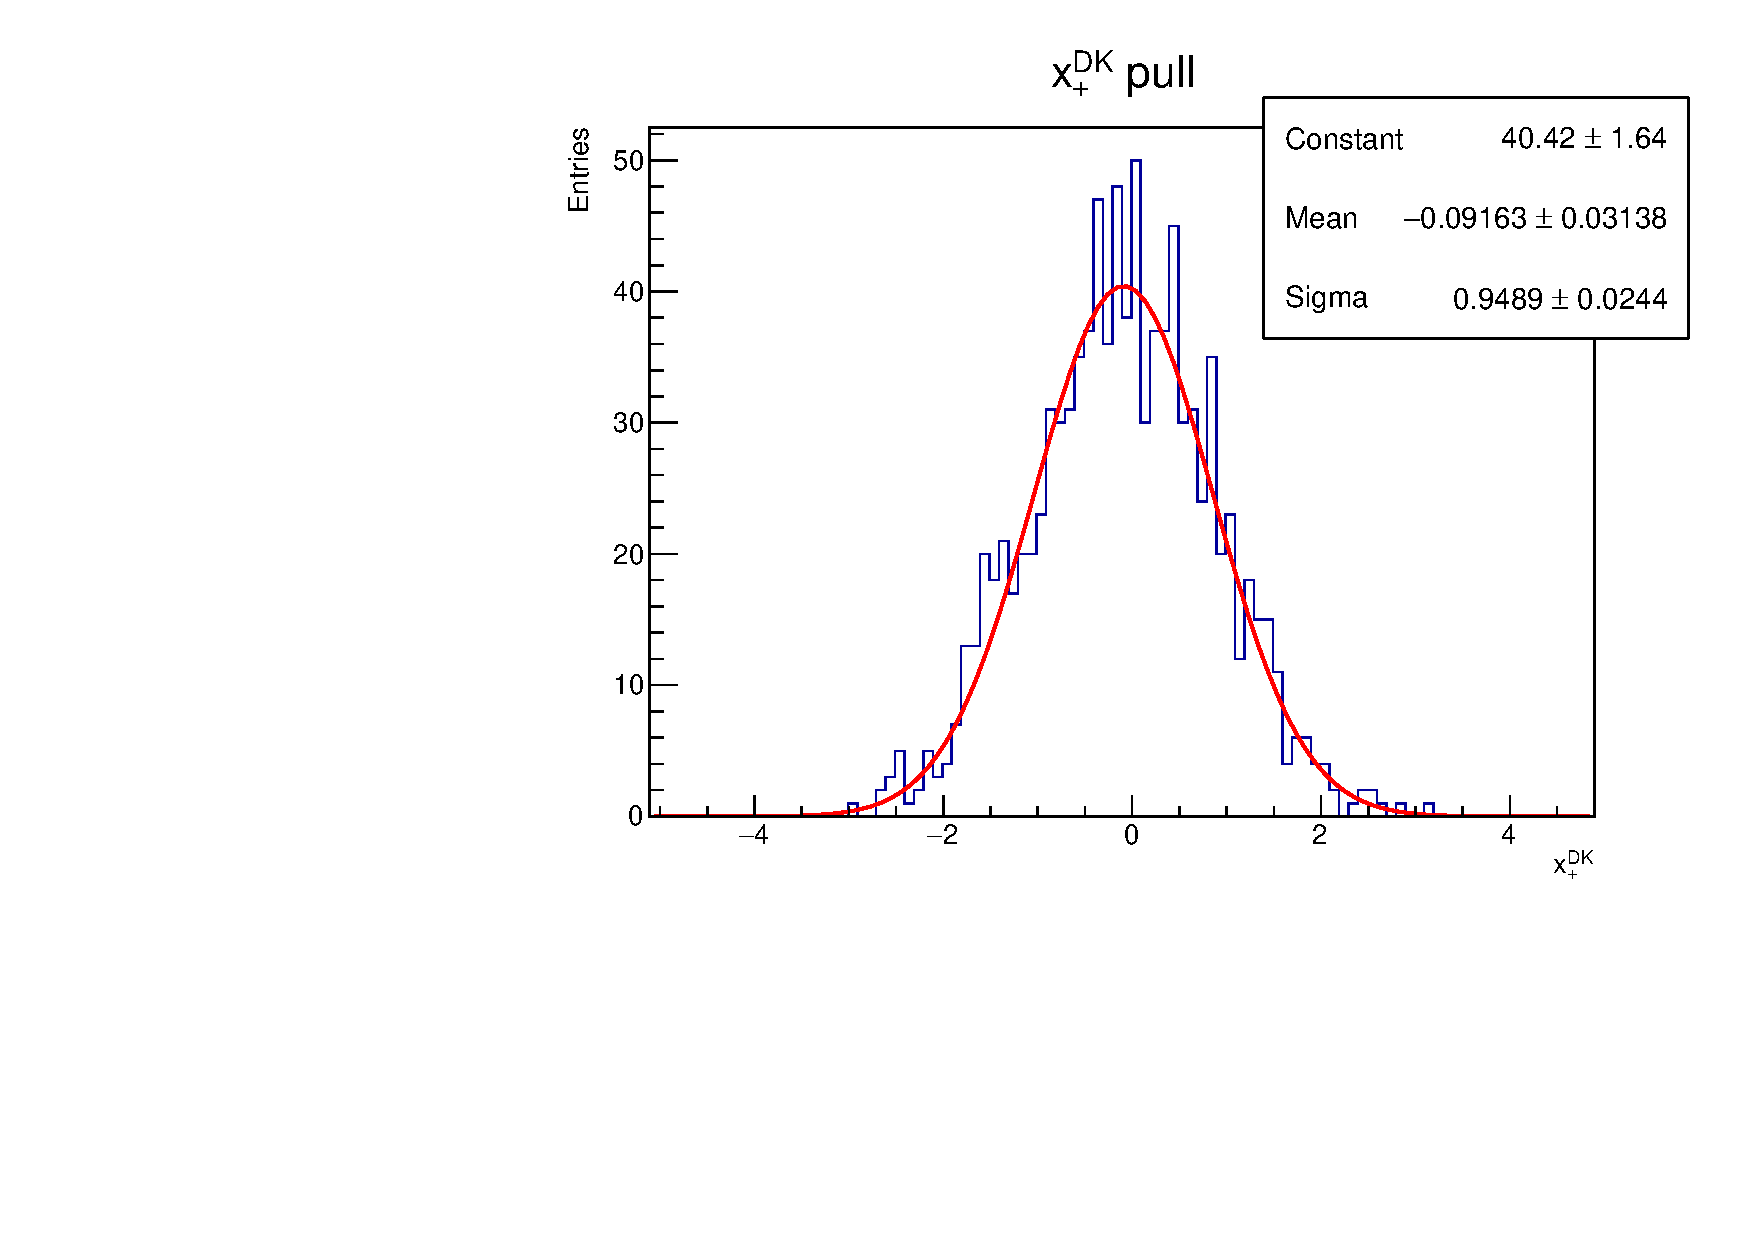
\includegraphics[width=1.0\textwidth]{Plots/A_xp_dk_pull.pdf}
      \vspace{-0.3cm}
      \caption*{$x_+^{DK}$}
    \end{subfigure}
    \caption*{$D^0\to K^+K^-\pi^+\pi^-$}
  \end{figure}
\end{frame}

\begin{frame}{CP fit toy studies}
  \begin{center}
    ...but $y_\pm^{DK}$ pulls are now slightly asymmetric!
  \end{center}
  \begin{figure}
    \centering
    \begin{subfigure}{0.5\textwidth}
      \centering
      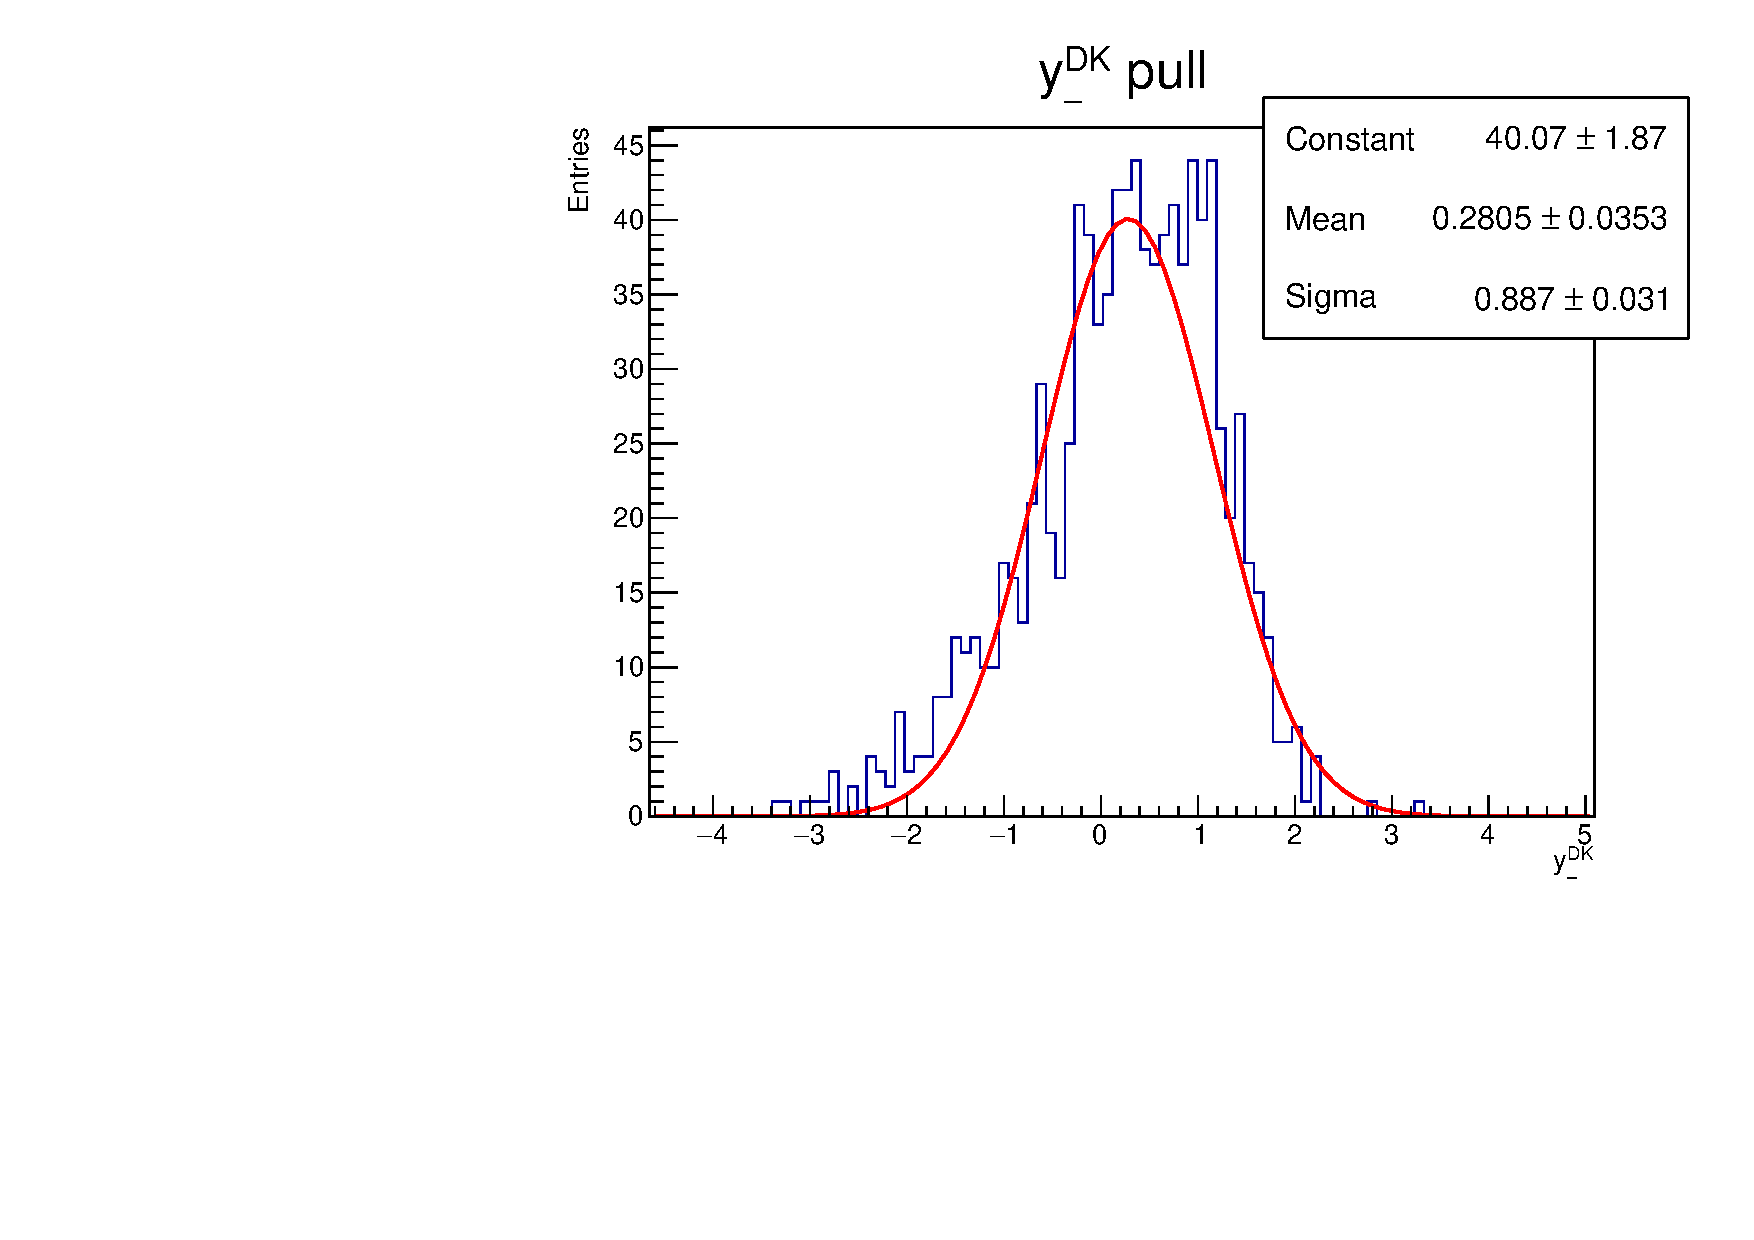
\includegraphics[width=1.0\textwidth]{Plots/A_ym_dk_pull.pdf}
      \vspace{-0.3cm}
      \caption*{$y_-^{DK}$}
    \end{subfigure}%
    \begin{subfigure}{0.5\textwidth}
      \centering
      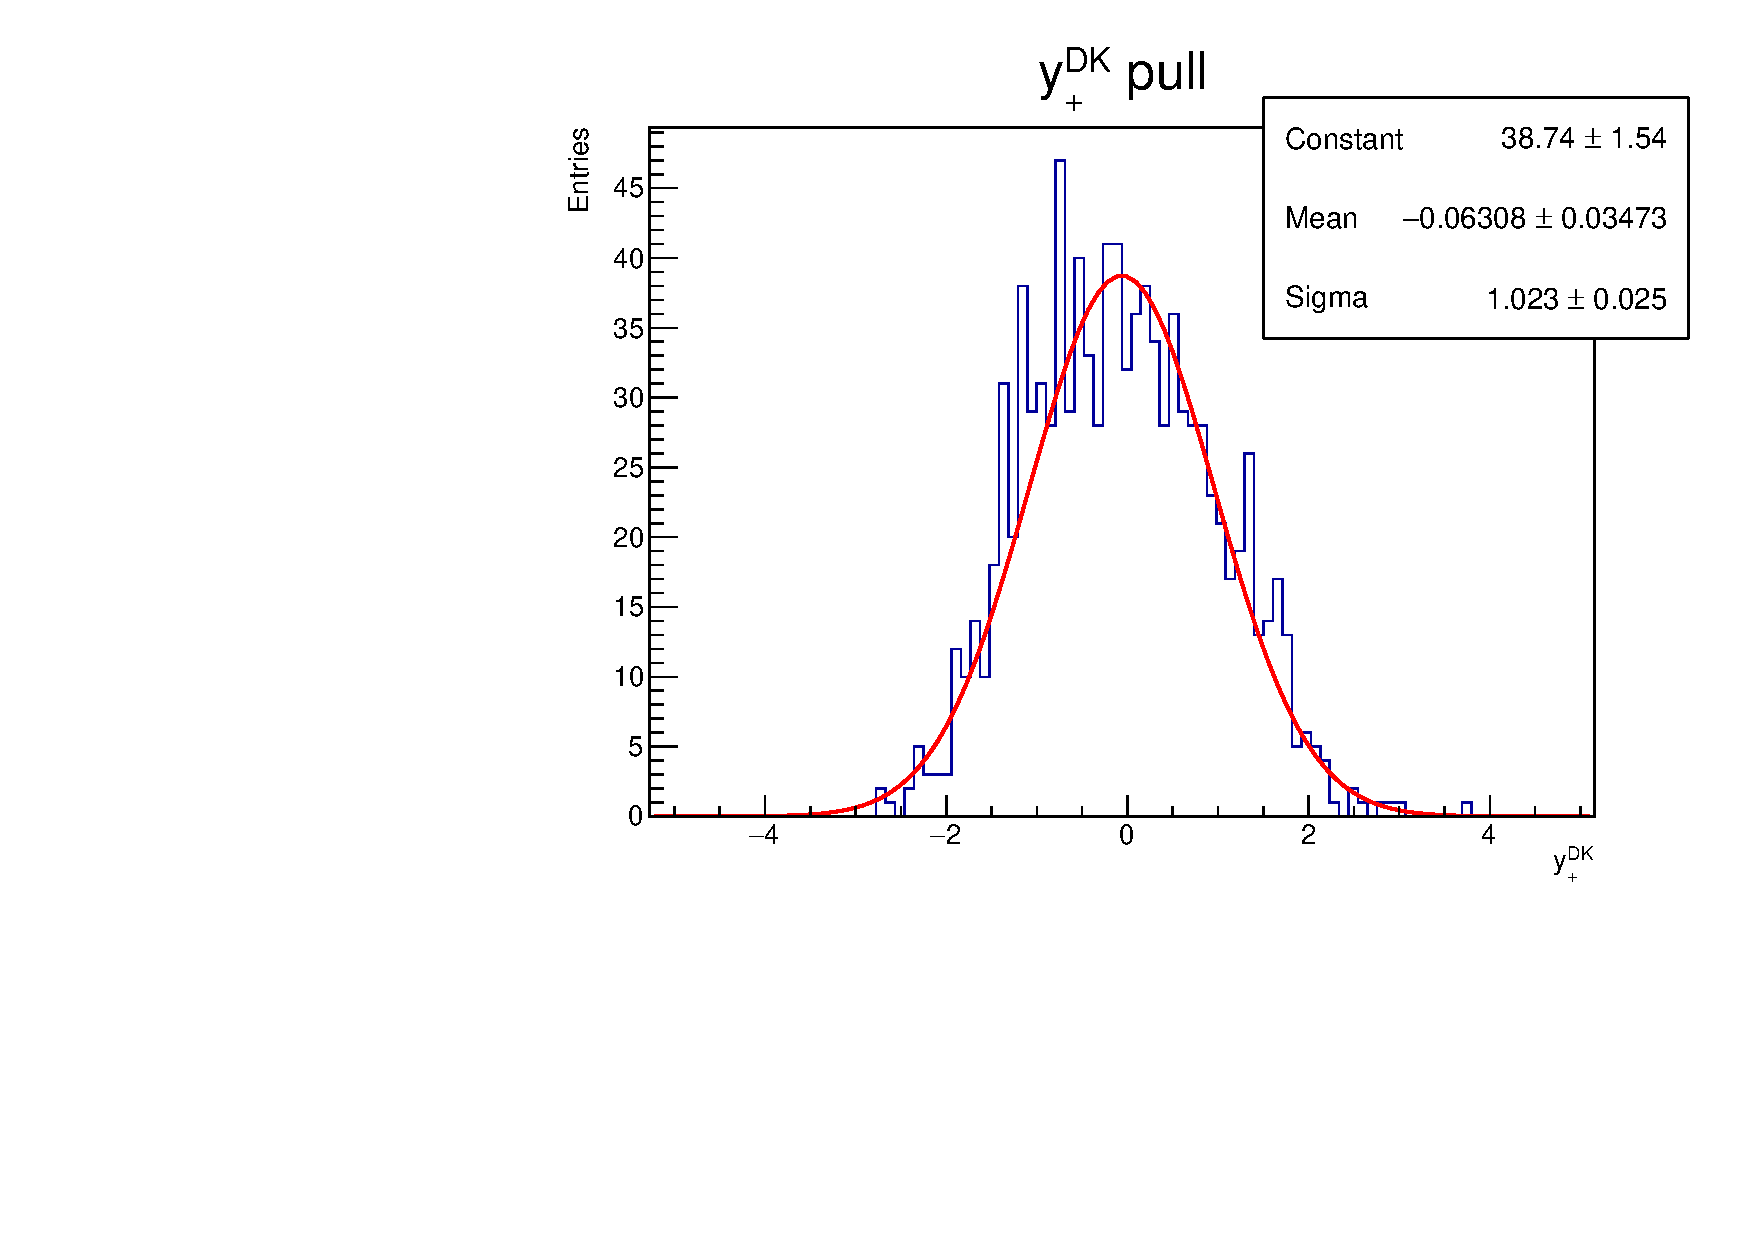
\includegraphics[width=1.0\textwidth]{Plots/A_yp_dk_pull.pdf}
      \vspace{-0.3cm}
      \caption*{$y_+^{DK}$}
    \end{subfigure}
    \caption*{$D^0\to K^+K^-\pi^+\pi^-$}
  \end{figure}
\end{frame}

\section{Likelihood scan of CP observables}
\begin{frame}{Strong-phase parameters in CP fit}
  \begin{center}
    {\large Why are $c_i$ and $s_i$ Gaussian constrained?}
  \end{center}
  \begin{itemize}
    \setlength\itemsep{1.0em}
    \item{Previous BPGGSZ analyses have kept $c_i$ and $s_i$ fixed}
    \begin{enumerate}
      \item{$c_i$ and $s_i$ uncertainties are added as a systematic through smearing}
      \item{Convenient for calculating correlations between different analyses}
      \item{Appropriate when $c_i$ and $s_i$ uncertainties are \underline{small}}
    \end{enumerate}
    \item{In four-body analyses, uncertainties on $\gamma$ from $c_i$ and $s_i$ are almost the same size as the statistical uncertainty}
    \item{$\gamma$ is found to move significantly between a fit where $c_i$ and $s_i$ are fixed and when they are constrained}
    \item{More importantly: Large $s_i$ uncertainties are found to introduce large non-Gaussian uncertainties on $s_i$}
  \end{itemize}
\end{frame}

\begin{frame}{Likelihood scan of CP observables}
  \begin{center}
    $x_\pm^{DK}$ agree well between likelihood scan and Hesse approximation
  \end{center}
  \begin{figure}
    \centering
    \begin{subfigure}{0.5\textwidth}
      \centering
      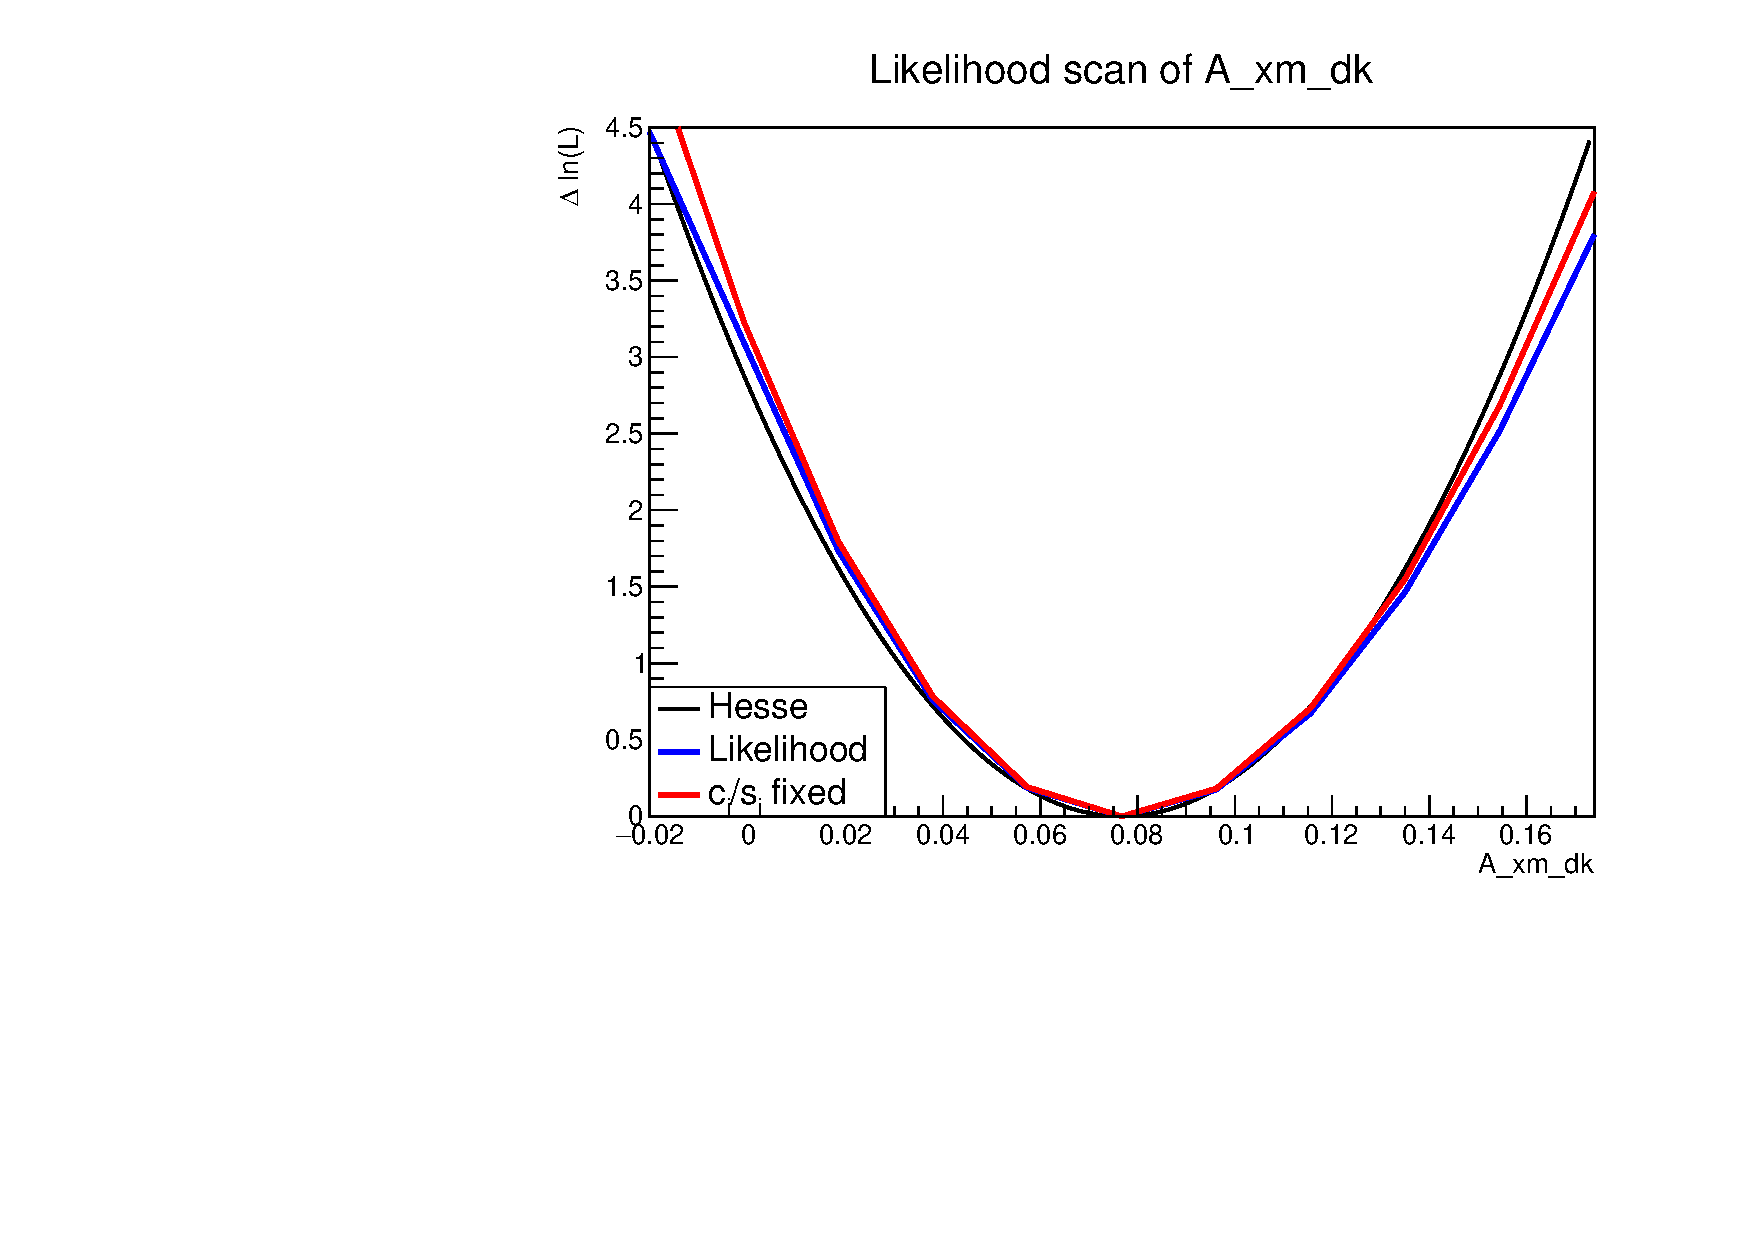
\includegraphics[width=1.0\textwidth]{Plots/A_xm_dk_likelihood_scan_KKpipi.pdf}
      \vspace{-0.3cm}
      \caption*{$x_-^{DK}$}
    \end{subfigure}%
    \begin{subfigure}{0.5\textwidth}
      \centering
      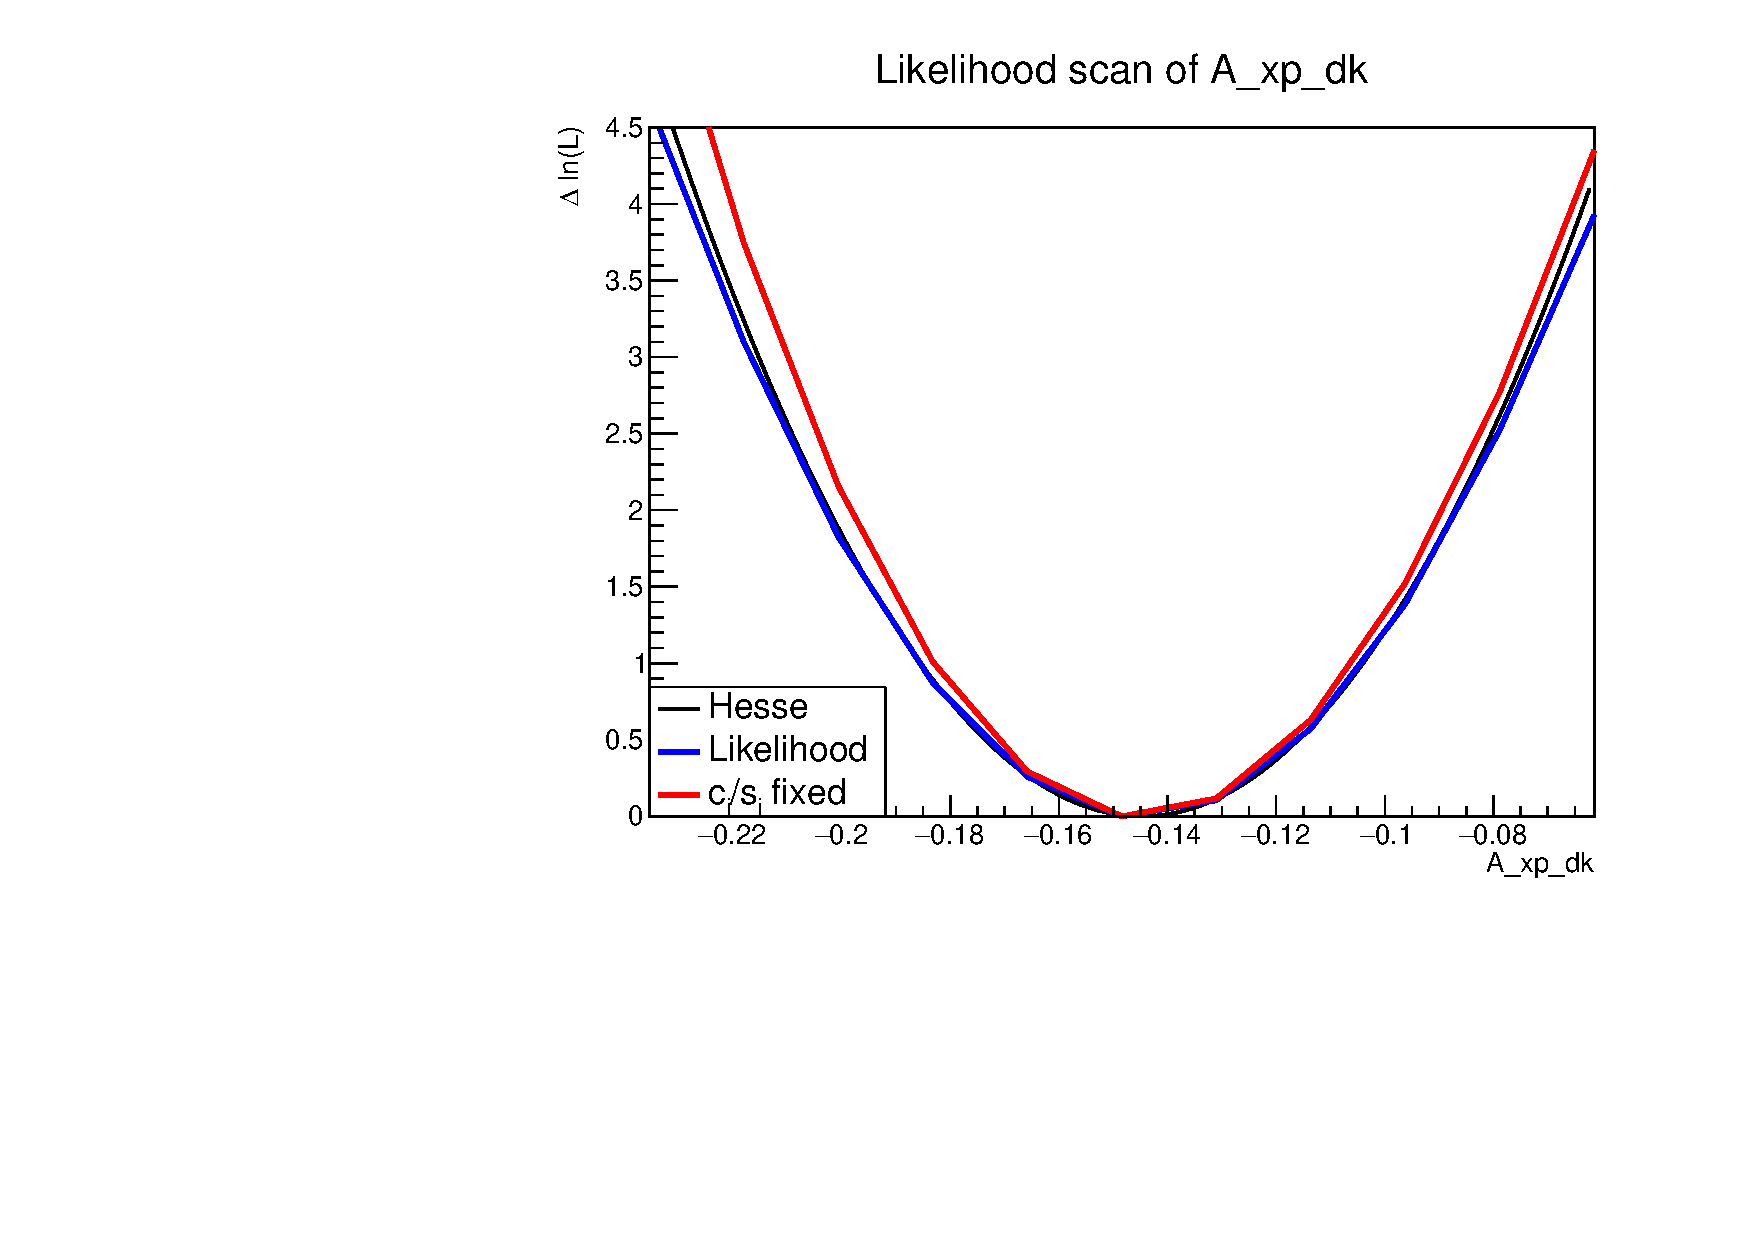
\includegraphics[width=1.0\textwidth]{Plots/A_xp_dk_likelihood_scan_KKpipi.pdf}
      \vspace{-0.3cm}
      \caption*{$x_+^{DK}$}
    \end{subfigure}
    \caption*{$D^0\to K^+K^-\pi^+\pi^-$}
  \end{figure}
\end{frame}

\begin{frame}{Likelihood scan of CP observables}
  \begin{center}
    $x_\pm^{DK}$ agree well between likelihood scan and Hesse approximation
  \end{center}
  \begin{figure}
    \centering
    \begin{subfigure}{0.5\textwidth}
      \centering
      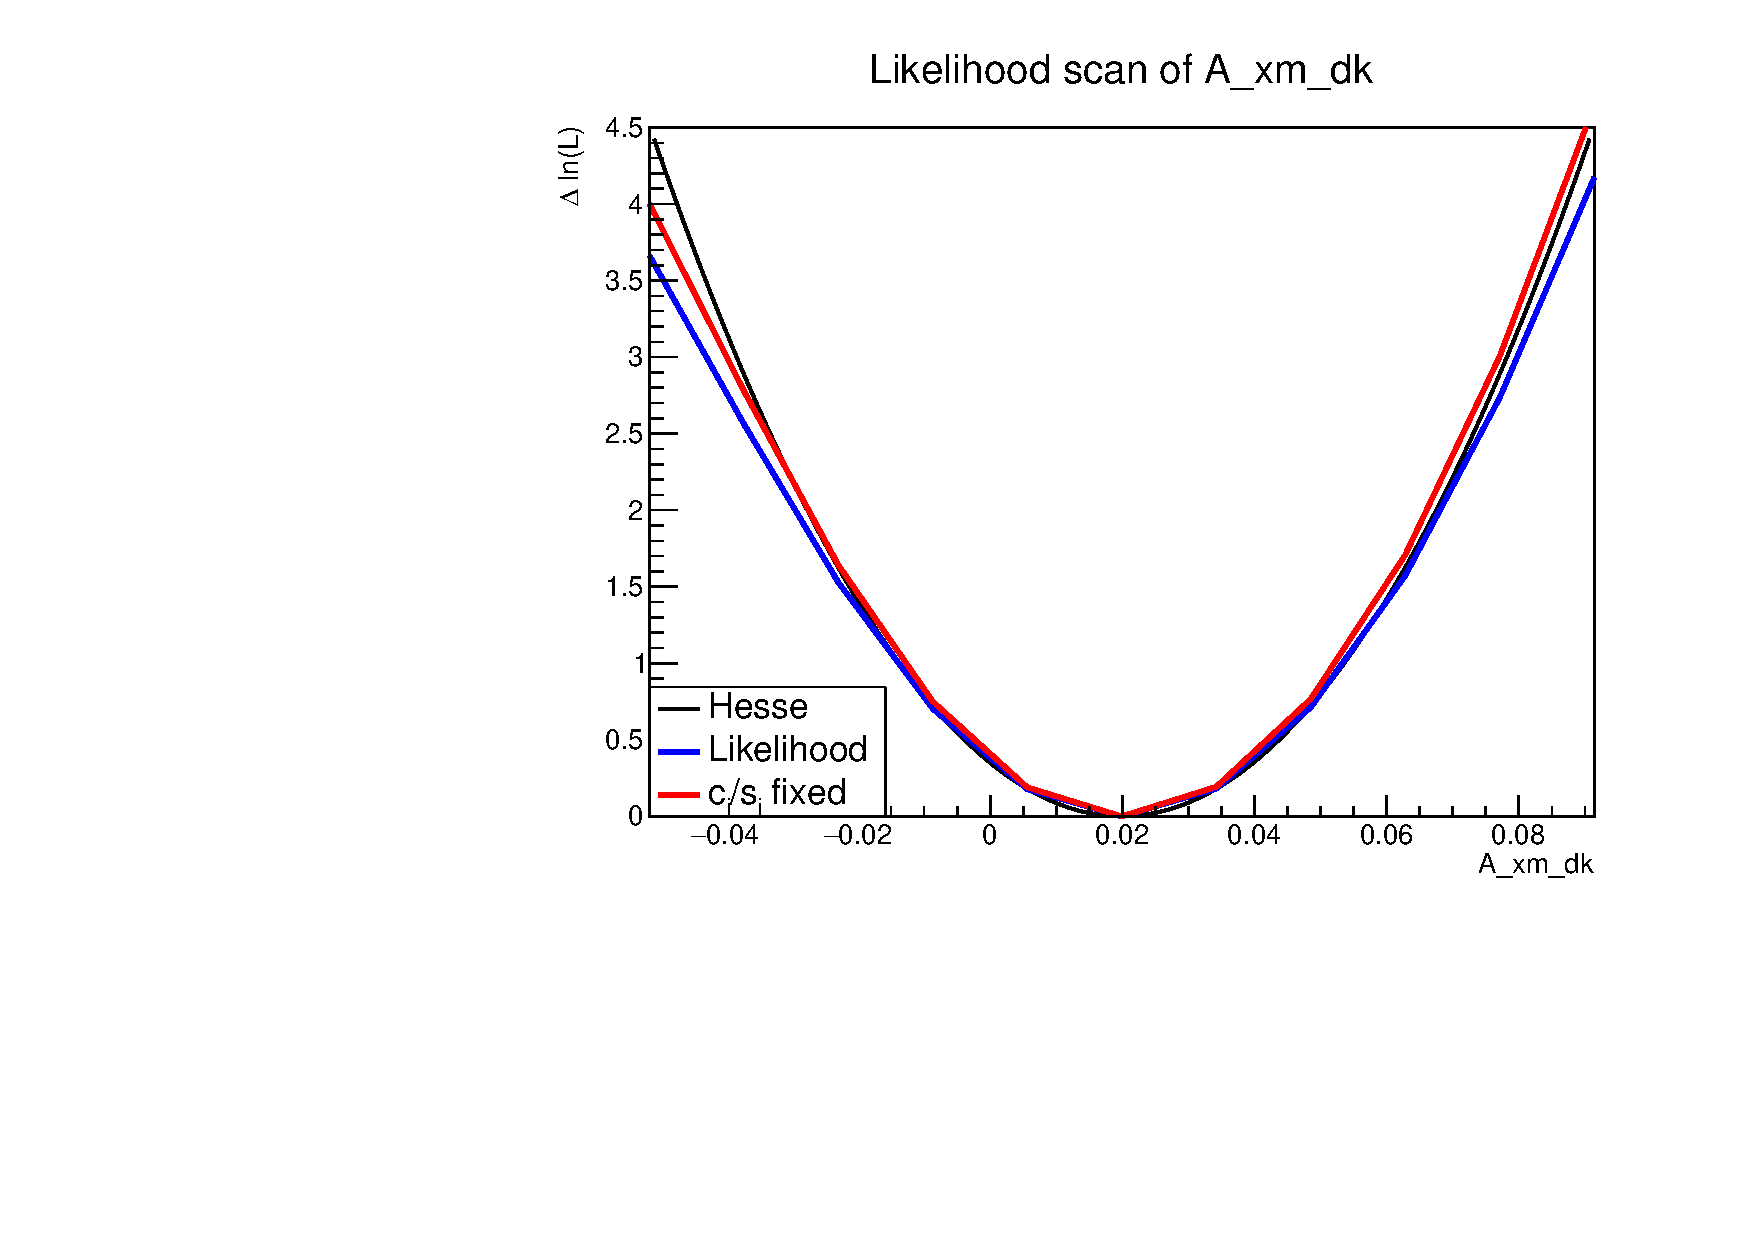
\includegraphics[width=1.0\textwidth]{Plots/A_xm_dk_likelihood_scan_pipipipi.pdf}
      \vspace{-0.3cm}
      \caption*{$x_-^{DK}$}
    \end{subfigure}%
    \begin{subfigure}{0.5\textwidth}
      \centering
      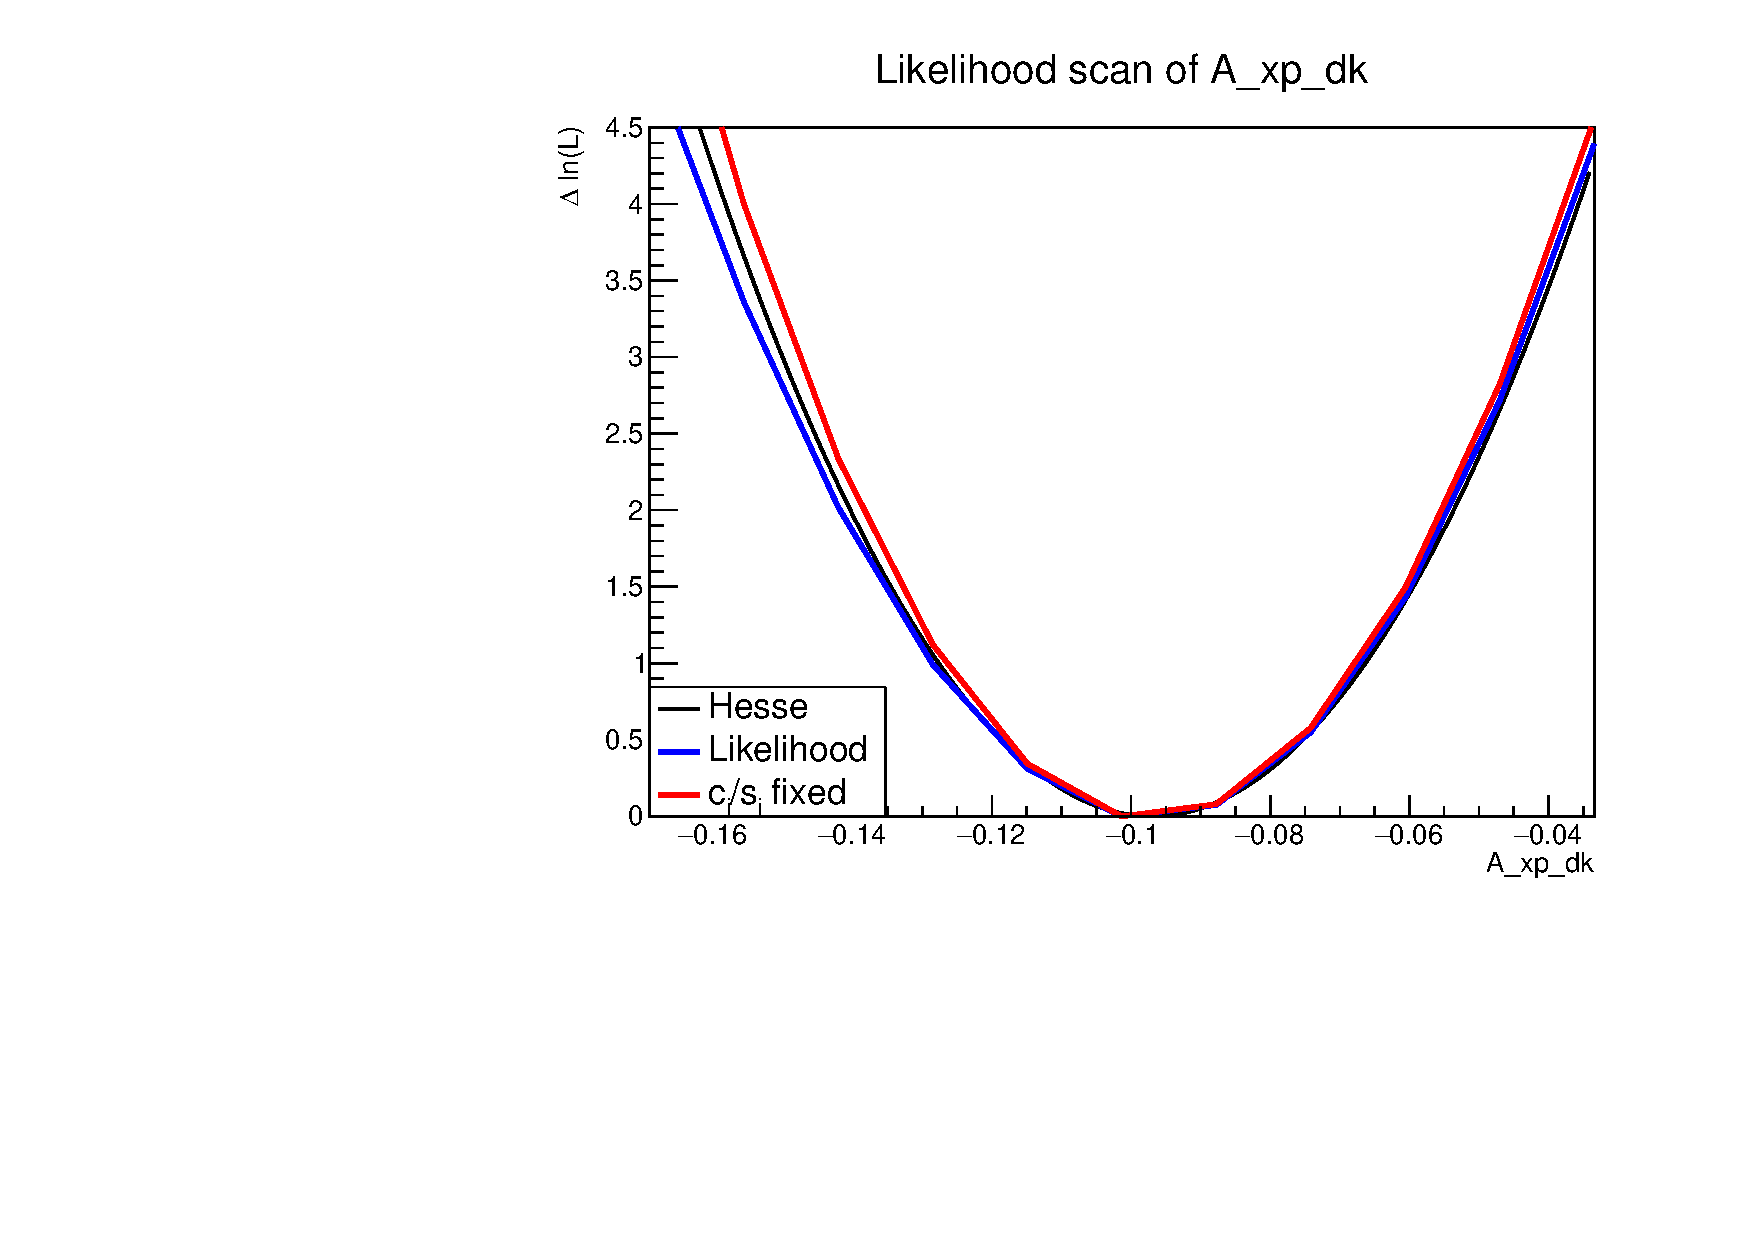
\includegraphics[width=1.0\textwidth]{Plots/A_xp_dk_likelihood_scan_pipipipi.pdf}
      \vspace{-0.3cm}
      \caption*{$x_+^{DK}$}
    \end{subfigure}
    \caption*{$D^0\to\pi^+\pi^-\pi^+\pi^-$}
  \end{figure}
\end{frame}

\begin{frame}{Likelihood scan of CP observables}
  \begin{center}
    $x_\pm^{DK}$ agree well between likelihood scan and Hesse approximation
  \end{center}
  \begin{figure}
    \centering
    \begin{subfigure}{0.5\textwidth}
      \centering
      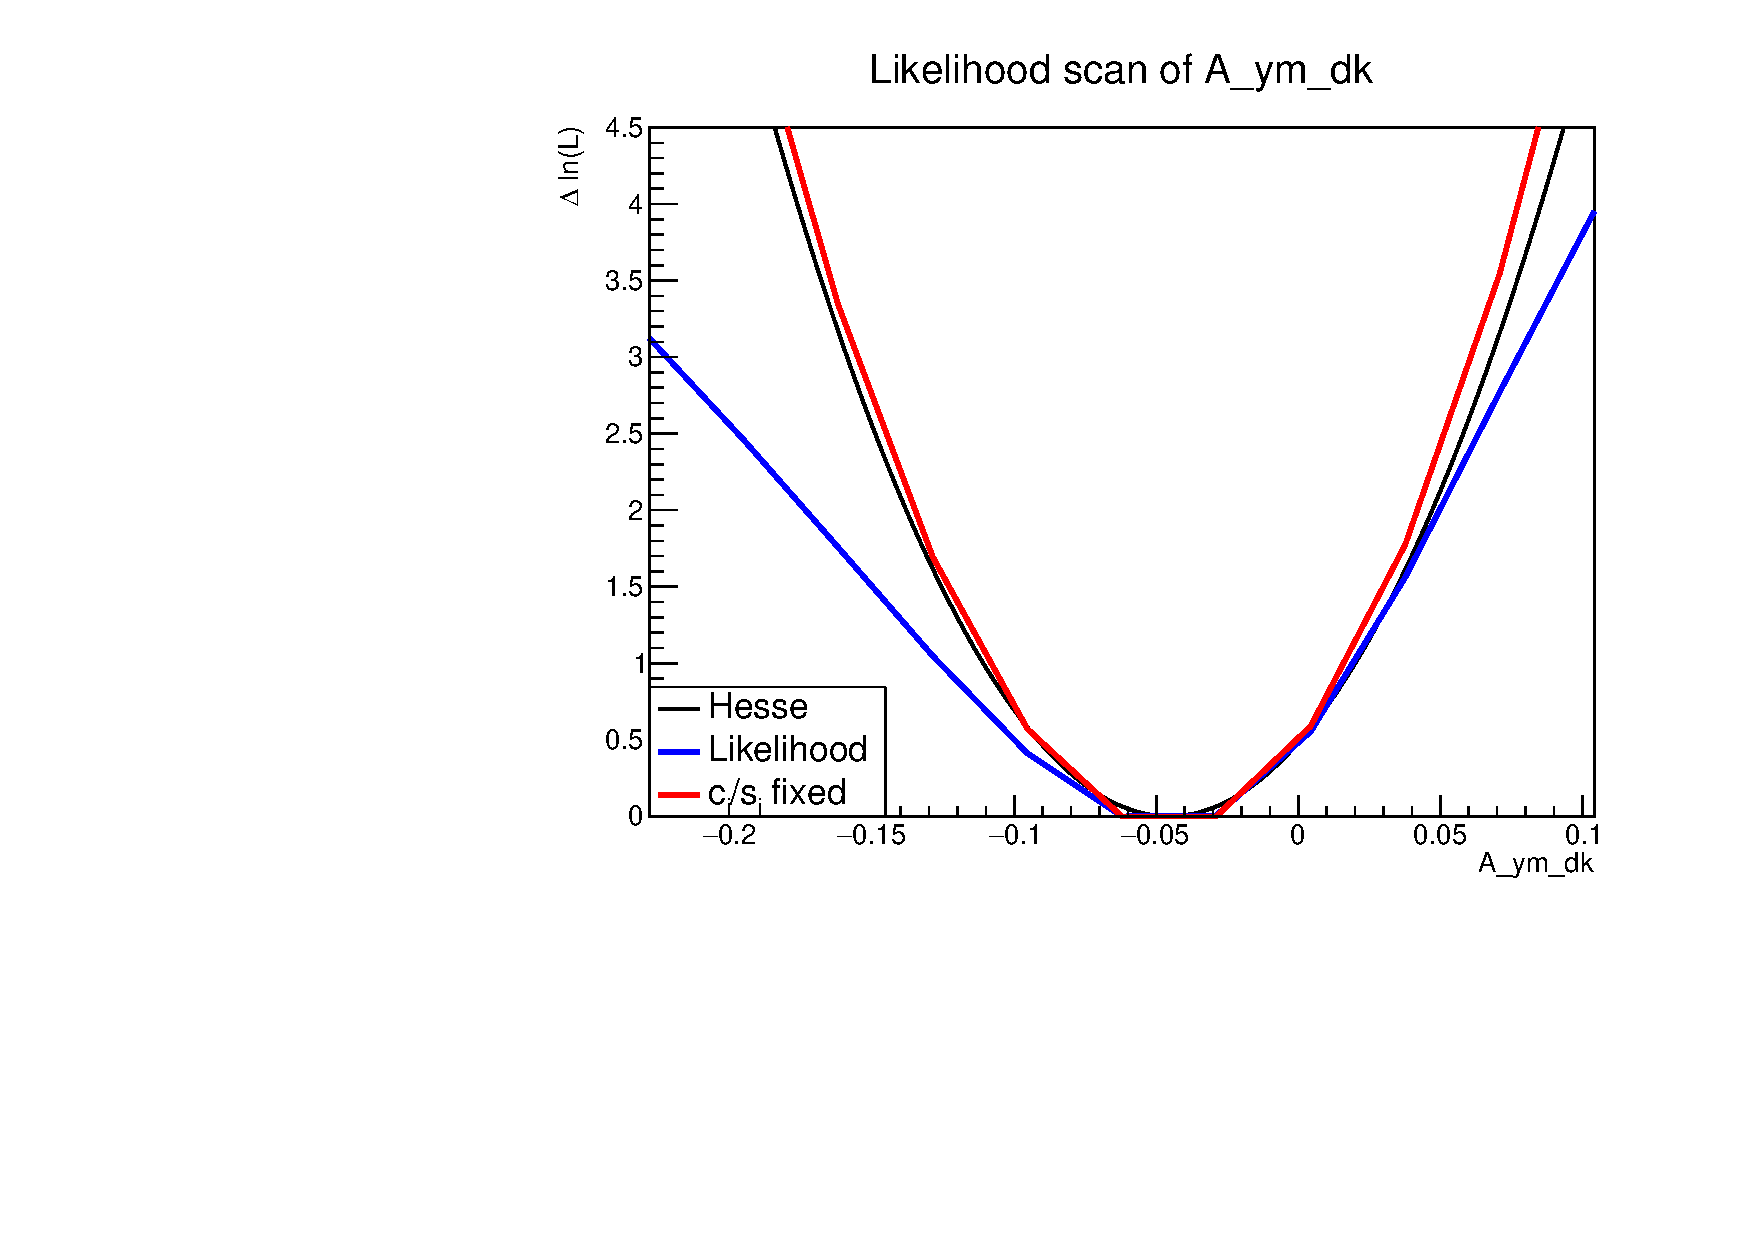
\includegraphics[width=1.0\textwidth]{Plots/A_ym_dk_likelihood_scan_KKpipi.pdf}
      \vspace{-0.3cm}
      \caption*{$y_-^{DK}$}
    \end{subfigure}%
    \begin{subfigure}{0.5\textwidth}
      \centering
      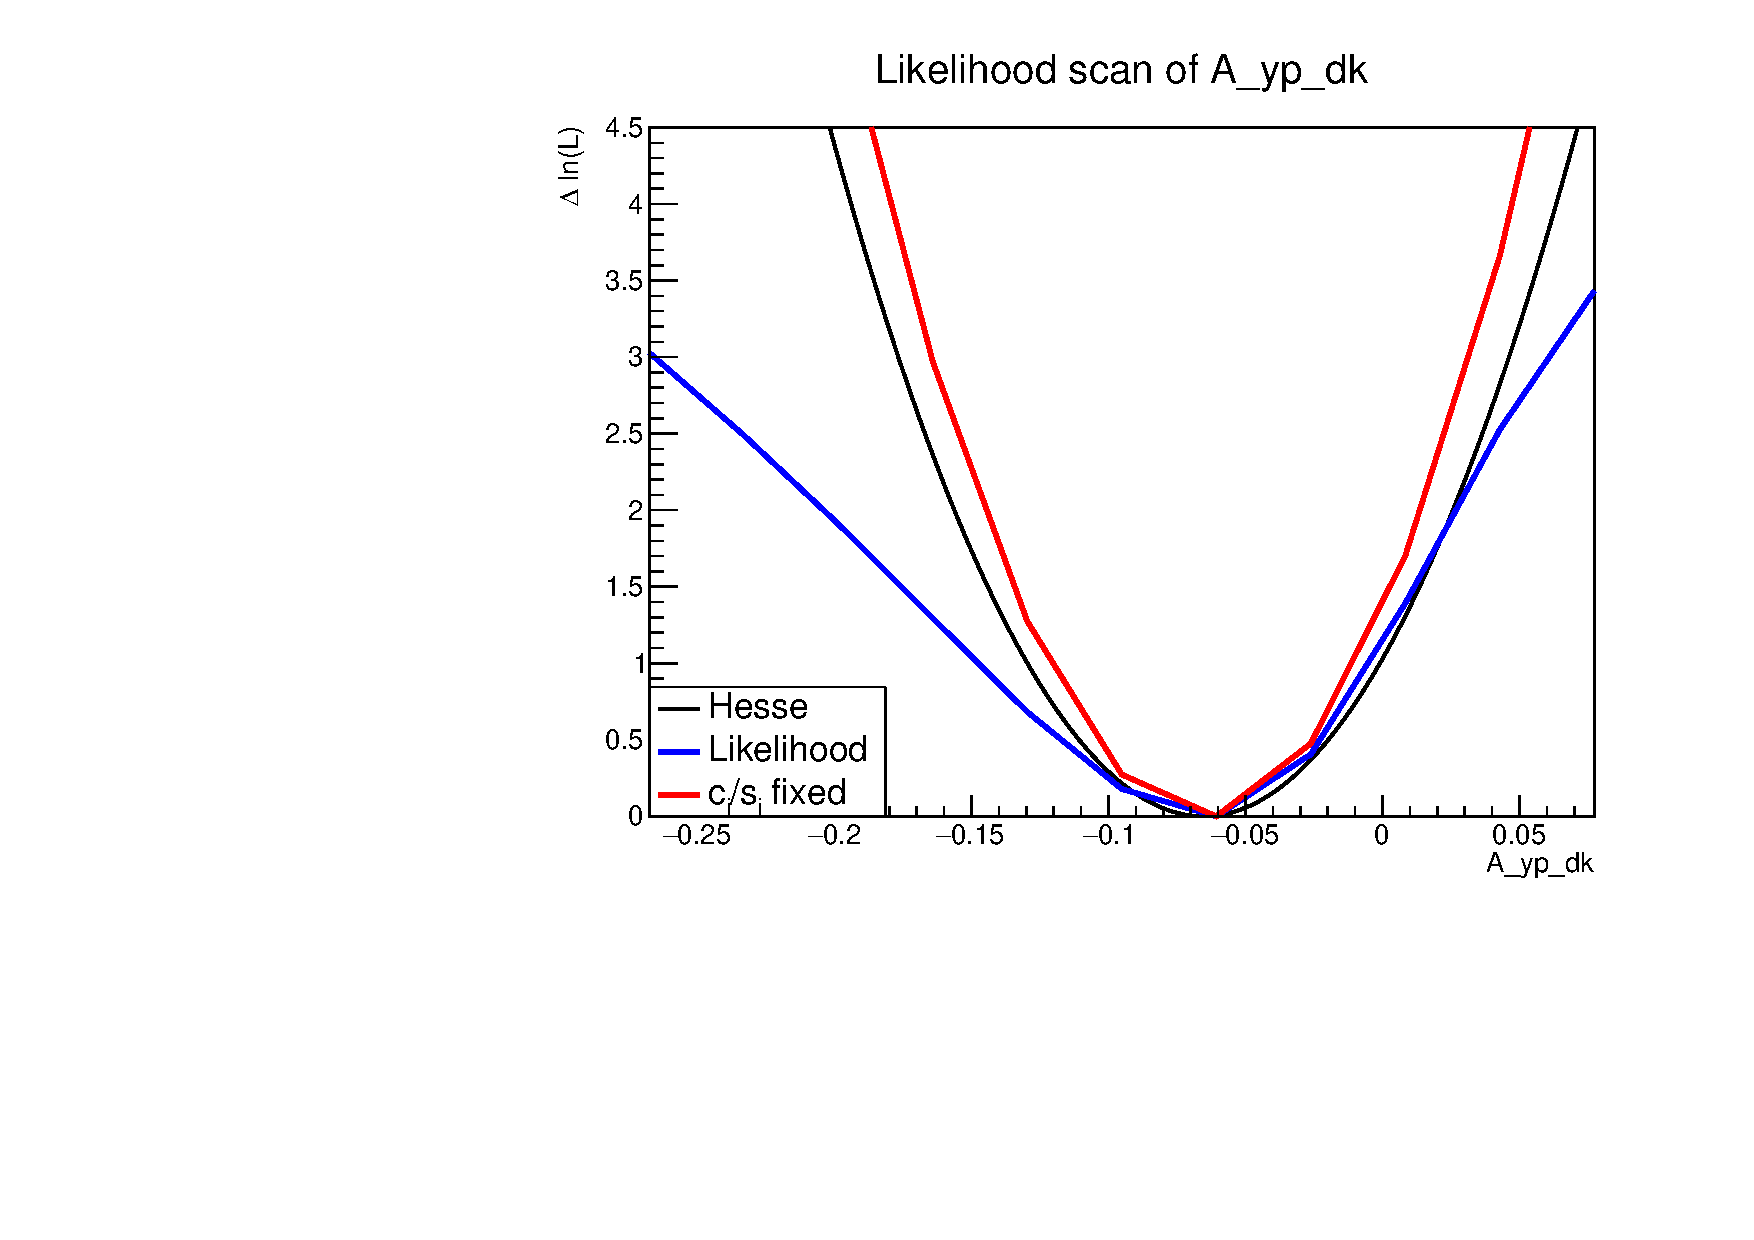
\includegraphics[width=1.0\textwidth]{Plots/A_yp_dk_likelihood_scan_KKpipi.pdf}
      \vspace{-0.3cm}
      \caption*{$y_+^{DK}$}
    \end{subfigure}
    \caption*{$D^0\to K^+K^-\pi^+\pi^-$}
  \end{figure}
\end{frame}

\begin{frame}{Likelihood scan of CP observables}
  \begin{center}
    $x_\pm^{DK}$ agree well between likelihood scan and Hesse approximation
  \end{center}
  \begin{figure}
    \centering
    \begin{subfigure}{0.5\textwidth}
      \centering
      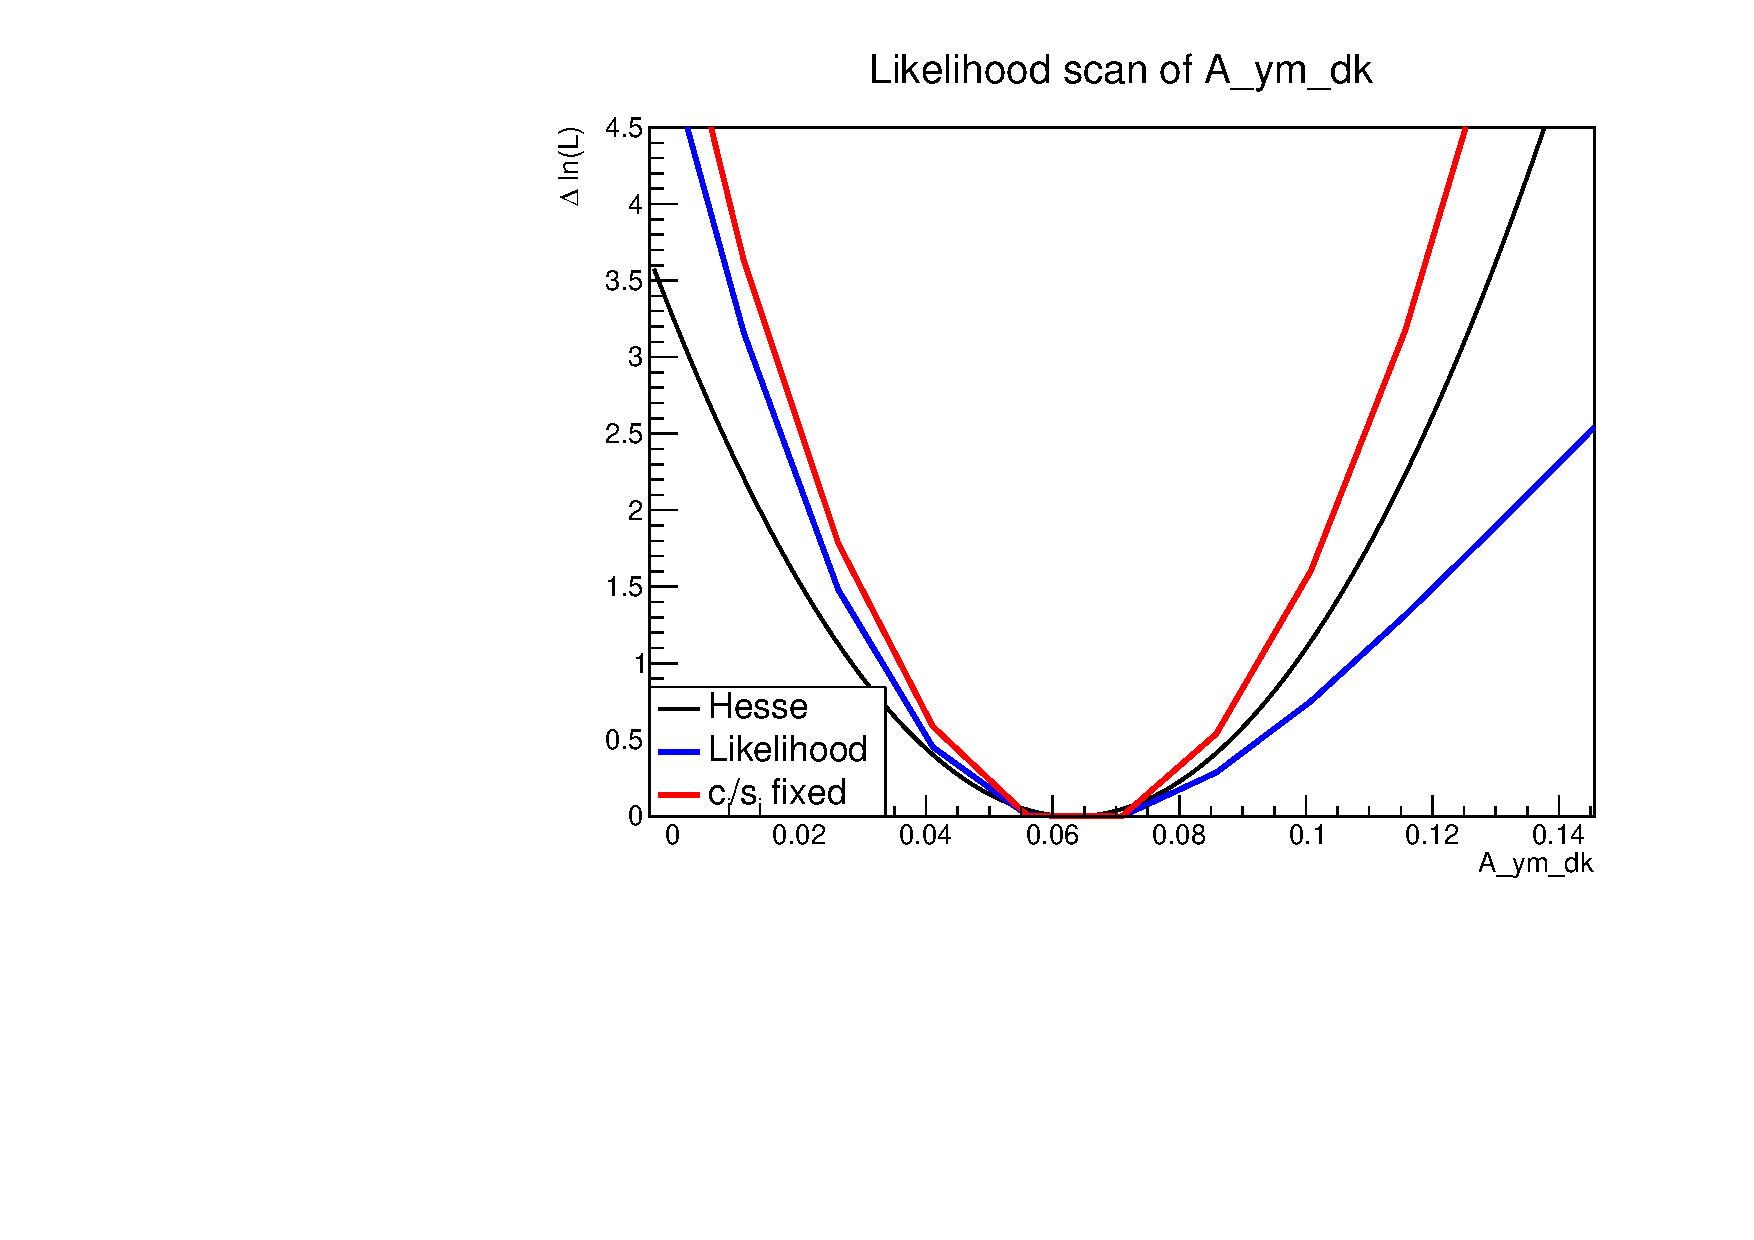
\includegraphics[width=1.0\textwidth]{Plots/A_ym_dk_likelihood_scan_pipipipi.pdf}
      \vspace{-0.3cm}
      \caption*{$y_-^{DK}$}
    \end{subfigure}%
    \begin{subfigure}{0.5\textwidth}
      \centering
      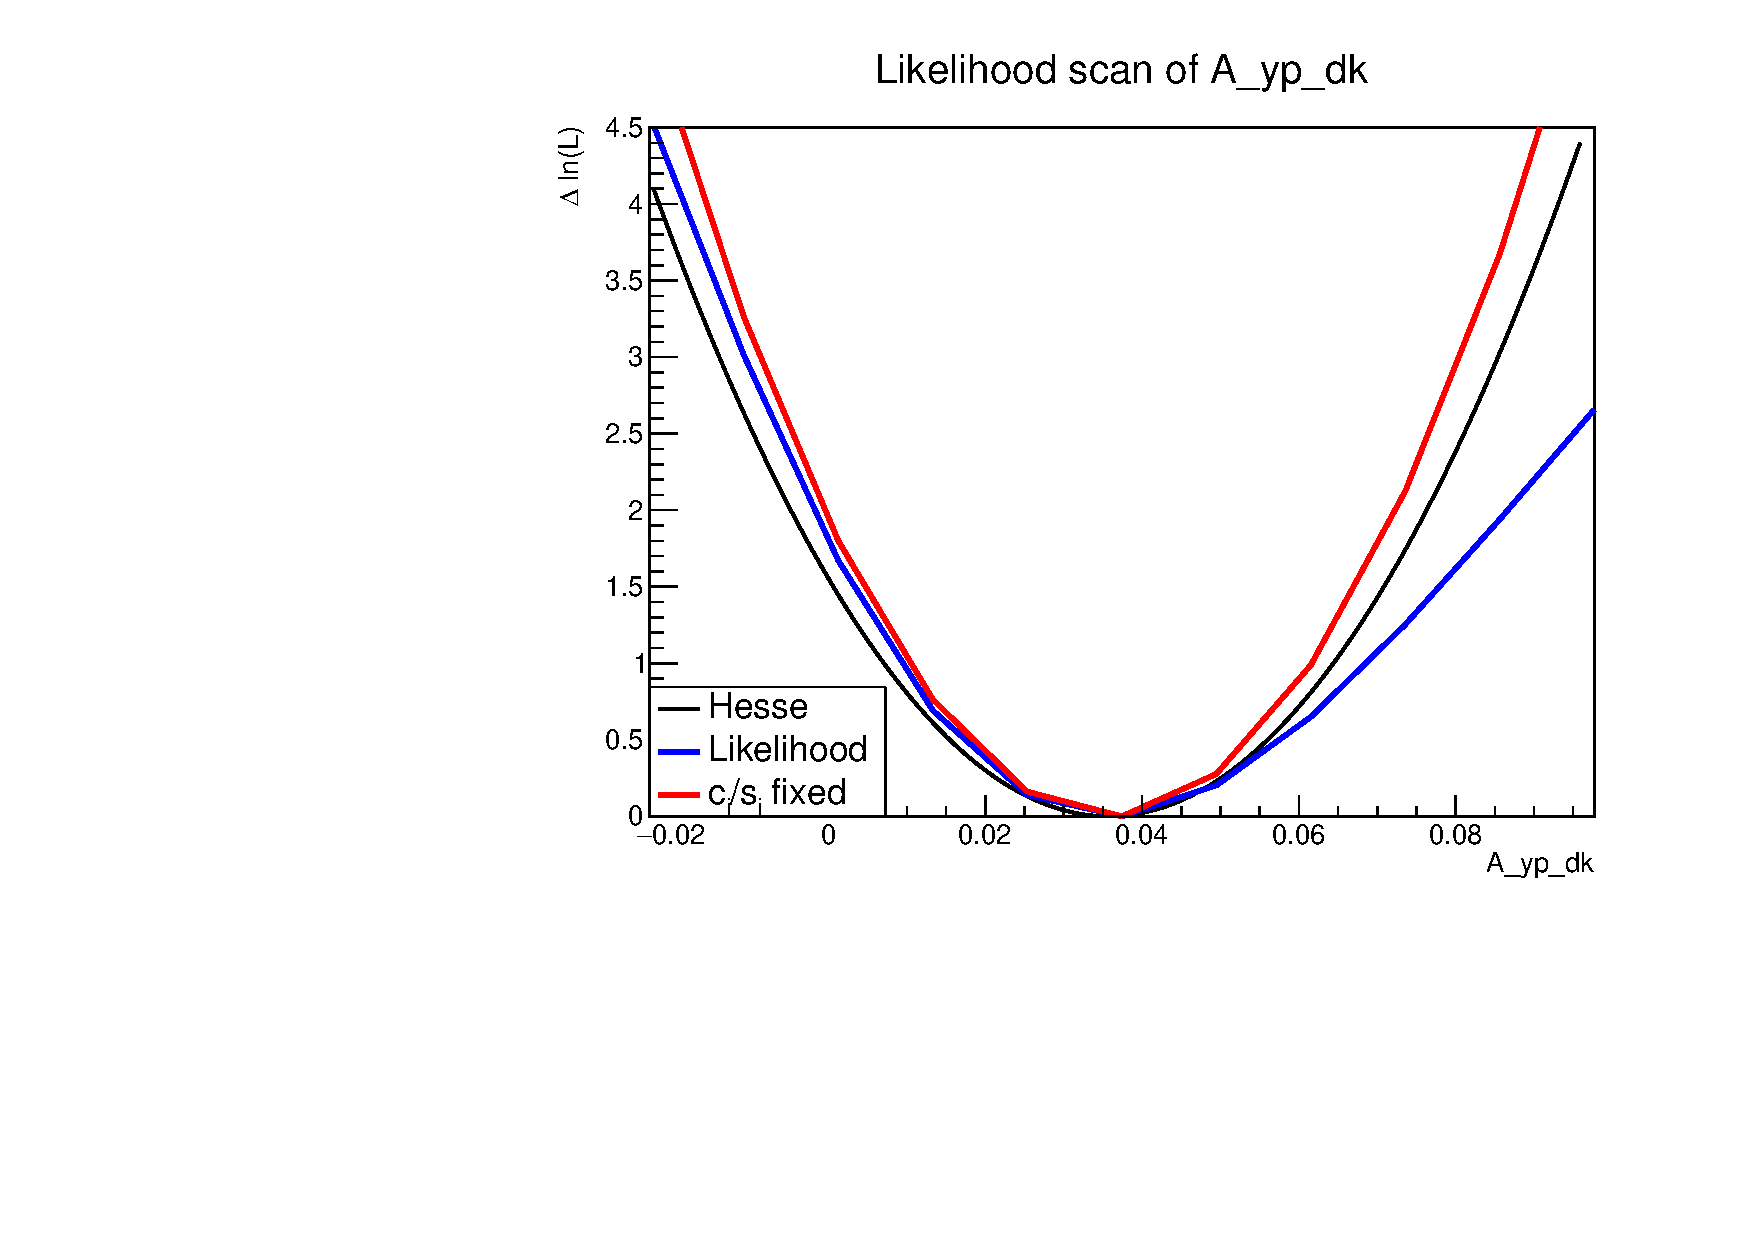
\includegraphics[width=1.0\textwidth]{Plots/A_yp_dk_likelihood_scan_pipipipi.pdf}
      \vspace{-0.3cm}
      \caption*{$y_+^{DK}$}
    \end{subfigure}
    \caption*{$D^0\to\pi^+\pi^-\pi^+\pi^-$}
  \end{figure}
\end{frame}

\begin{frame}{Likelihood scan of CP observables}
  \begin{center}
    {\large What do the likelihood scans tell us?}
  \end{center}
  \begin{itemize}
    \setlength\itemsep{1.5em}
    \item{Uncertainties from $c_i$ and $s_i$ are significant, which justifies Gaussian constraining $c_i$ and $s_i$}
    \item{Non-Gaussian uncertainties means GammaCombo cannot be used}
    \item{New strategy:}
    \begin{enumerate}
      \setlength\itemsep{0.5em}
      \item{Produce a likelihood function from CP fit}
      \item{Interpret CP observables in terms of $\gamma$, etc}
      \item{Must \underline{profile} all nuisance parameters ($F_i$, $c_i$, $s_i$, backgrounds yields, normalisation constants)}
      \item{Provide direct measurements of $\gamma$, $\delta_B$ and $r_B$ without GammaCombo}
    \end{enumerate}
  \end{itemize}
\end{frame}

\section{Systematic uncertainties}
\begin{frame}{Summary of LHCb internal systematic uncertainties}
  \begin{center}
    Internal LHCb systematic uncertainties from model-dependent analysis:
  \end{center}
  \vspace{-0.3cm}
  \scriptsize
  \vspace{0.02cm}
  \begin{center}
    \begin{tabular}{lcccccc}
        \hline
        Source & $x_-^{DK}$ & $y_-^{DK}$ & $x_+^{DK}$ & $y_+^{DK}$ & $x_\xi^{D\pi}$ & $y_\xi^{D\pi}$ \\
        \hline
        Statistical                                                & $2.87$ & $3.40$ & $2.51$ & $3.05$ & $4.24$ & $5.17$ \\
        \hline
        Mass shape                                                 & $0.02$ & $0.02$ & $0.03$ & $0.06$ & $0.02$ & $0.04$ \\
        Bin-dependent mass shape                                   & $0.11$ & $0.05$ & $0.10$ & $0.19$ & $0.68$ & $0.16$ \\
        PID efficiency                                             & $0.02$ & $0.02$ & $0.03$ & $0.06$ & $0.02$ & $0.04$ \\
        Low-mass background model                                  & $0.02$ & $0.02$ & $0.03$ & $0.04$ & $0.02$ & $0.02$ \\
        Charmless background                                       & $0.14$ & $0.15$ & $0.12$ & $0.14$ & $0.01$ & $0.02$ \\
        $C\!P$ violation in low-mass background                    & $0.01$ & $0.10$ & $0.08$ & $0.12$ & $0.07$ & $0.26$ \\
        Semi-leptonic $b$-hadron decays                            & $0.05$ & $0.27$ & $0.06$ & $0.01$ & $0.07$ & $0.19$ \\
        Semi-leptonic charm decays                                 & $0.02$ & $0.07$ & $0.03$ & $0.15$ & $0.06$ & $0.24$ \\
        $D\to K^-\pi^+\pi^-\pi^+$ background                       & $0.11$ & $0.05$ & $0.07$ & $0.04$ & $0.09$ & $0.05$ \\
        $\Lambda_b\to pD\pi^-$ background                          & $0.01$ & $0.25$ & $0.14$ & $0.04$ & $0.06$ & $0.34$ \\
        $D\to K^-\pi^+\pi^-\pi^+\pi^0$ background                  & $0.30$ & $0.05$ & $0.19$ & $0.07$ & $0.05$ & $0.01$ \\
        Fit bias                                                   & $0.06$ & $0.05$ & $0.13$ & $0.02$ & $0.06$ & $0.13$ \\
        \hline
        Total LHCb systematic                                      & $0.37$ & $0.43$ & $0.34$ & $0.32$ & $0.70$ & $0.57$ \\
        \hline
    \end{tabular}
  \end{center}
  \begin{center}
    {\normalsize Give systematic uncertainties in terms of CP observables (not $\gamma$) since these are more Gaussian and better behaved}
  \end{center}
\end{frame}

\section{Interpretation}
\begin{frame}{Interpretation strategy}
  \begin{center}
    {\large From CP fit, we have a (negative log) likelihood function with nuisance parameters $n_k$:}
  \end{center}
  \begin{equation*}
    \mathcal{L}(x_-^{DK}, y_-^{DK}, x_+^{DK}, y_+^{DK}, x_\xi^{D\pi}, y_\xi^{D\pi}, \{n_k\})
  \end{equation*}
  \vspace{0.1cm}
  \begin{center}
    {\large Express in terms of physics parameters:}
  \end{center}
  \begin{equation*}
    \mathcal{L}(\gamma, \delta_B^{DK}, r_B^{DK}, \delta_B^{D\pi}, r_B^{D\pi}, \{n_k\})
  \end{equation*}
  \vspace{0.1cm}
  \begin{center}
    {\normalsize In this step, also add a Gaussian smearing term on CP observables to account for internal LHCb systematics}
  \end{center}
\end{frame}

\begin{frame}{Interpretation toys}
  \begin{center}
    We can perform toy studies on the interpretation fit, but we do \underline{not} expect these to behave very Gaussian...
  \end{center}
  \begin{figure}
    \centering
    \begin{subfigure}{0.5\textwidth}
      \centering
      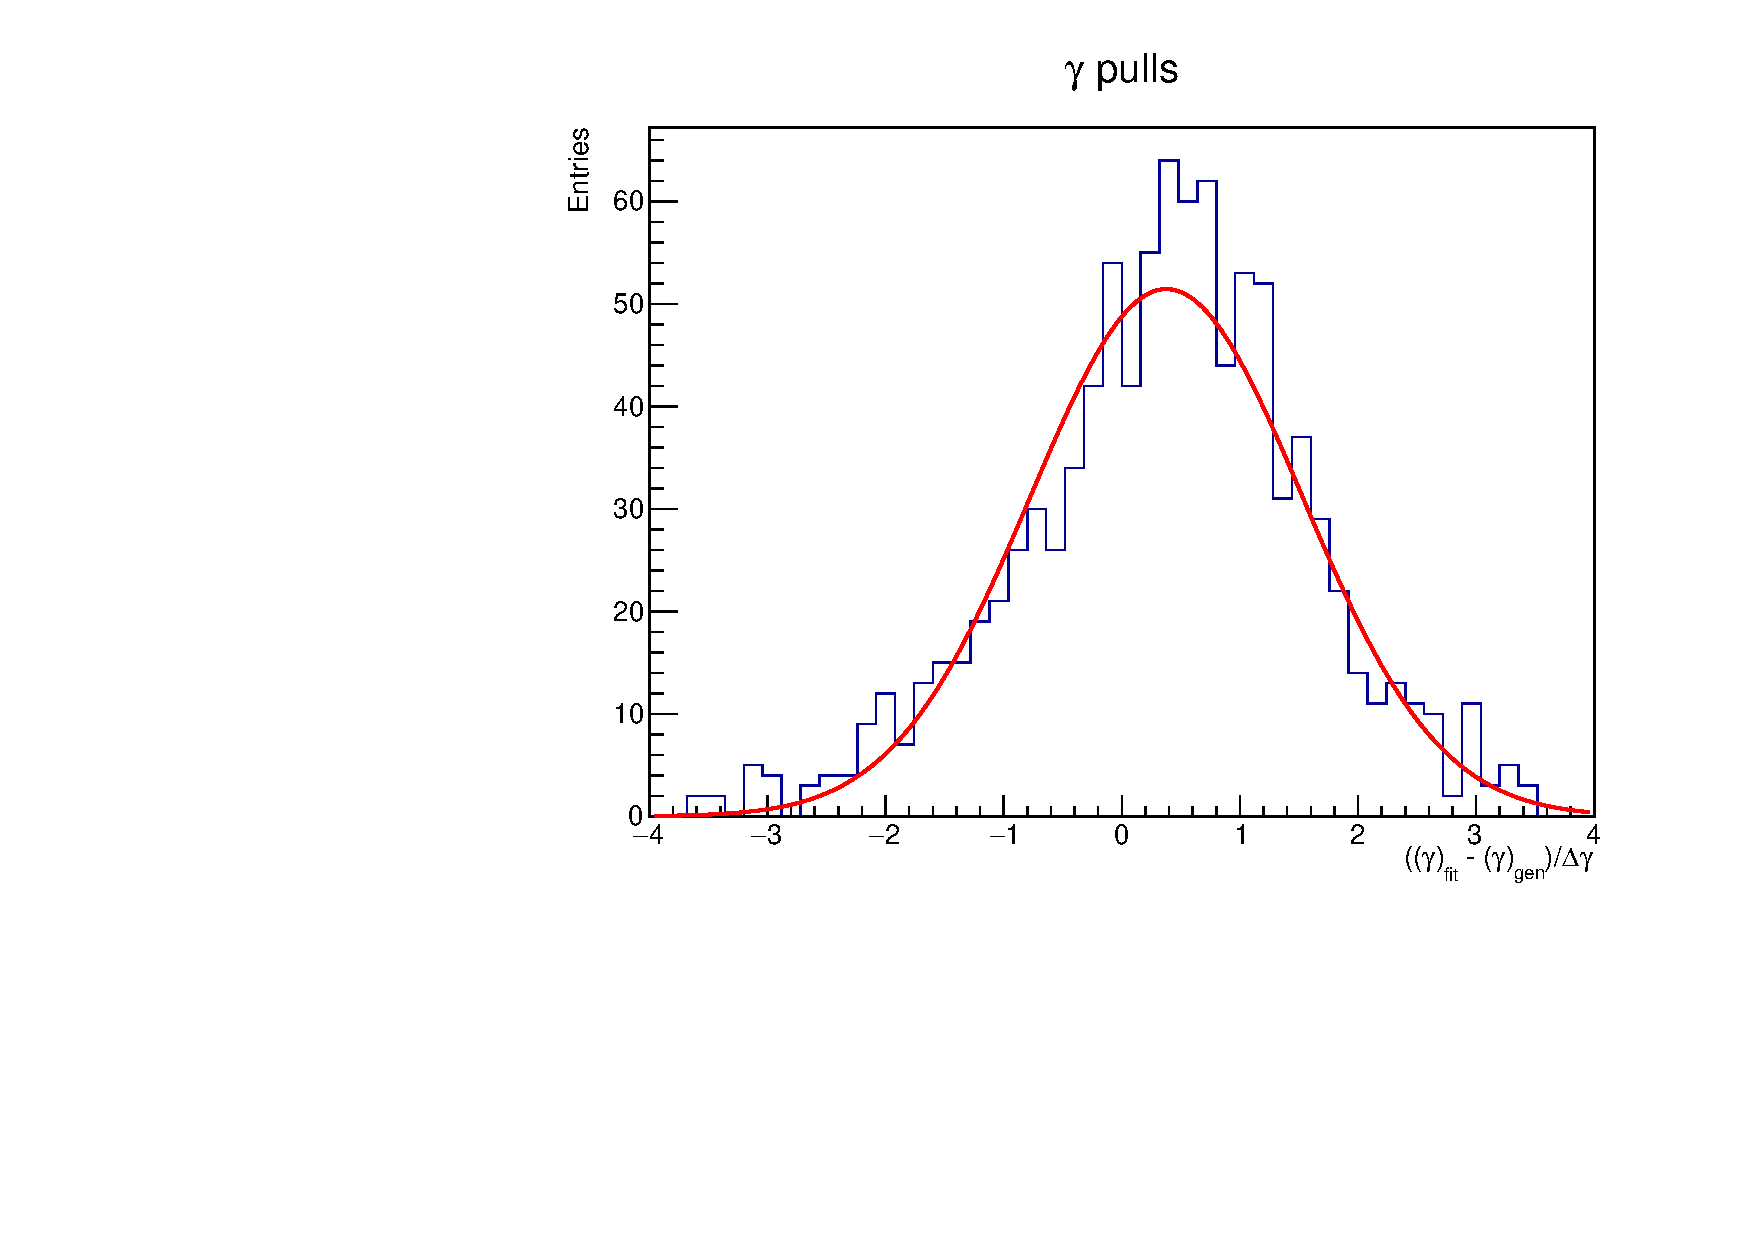
\includegraphics[width=1.0\textwidth]{Plots/gamma_pull_toys_KKpipi.pdf}
      \vspace{-0.3cm}
      \caption*{$K^+K^-\pi^+\pi^-$}
    \end{subfigure}%
    \begin{subfigure}{0.5\textwidth}
      \centering
      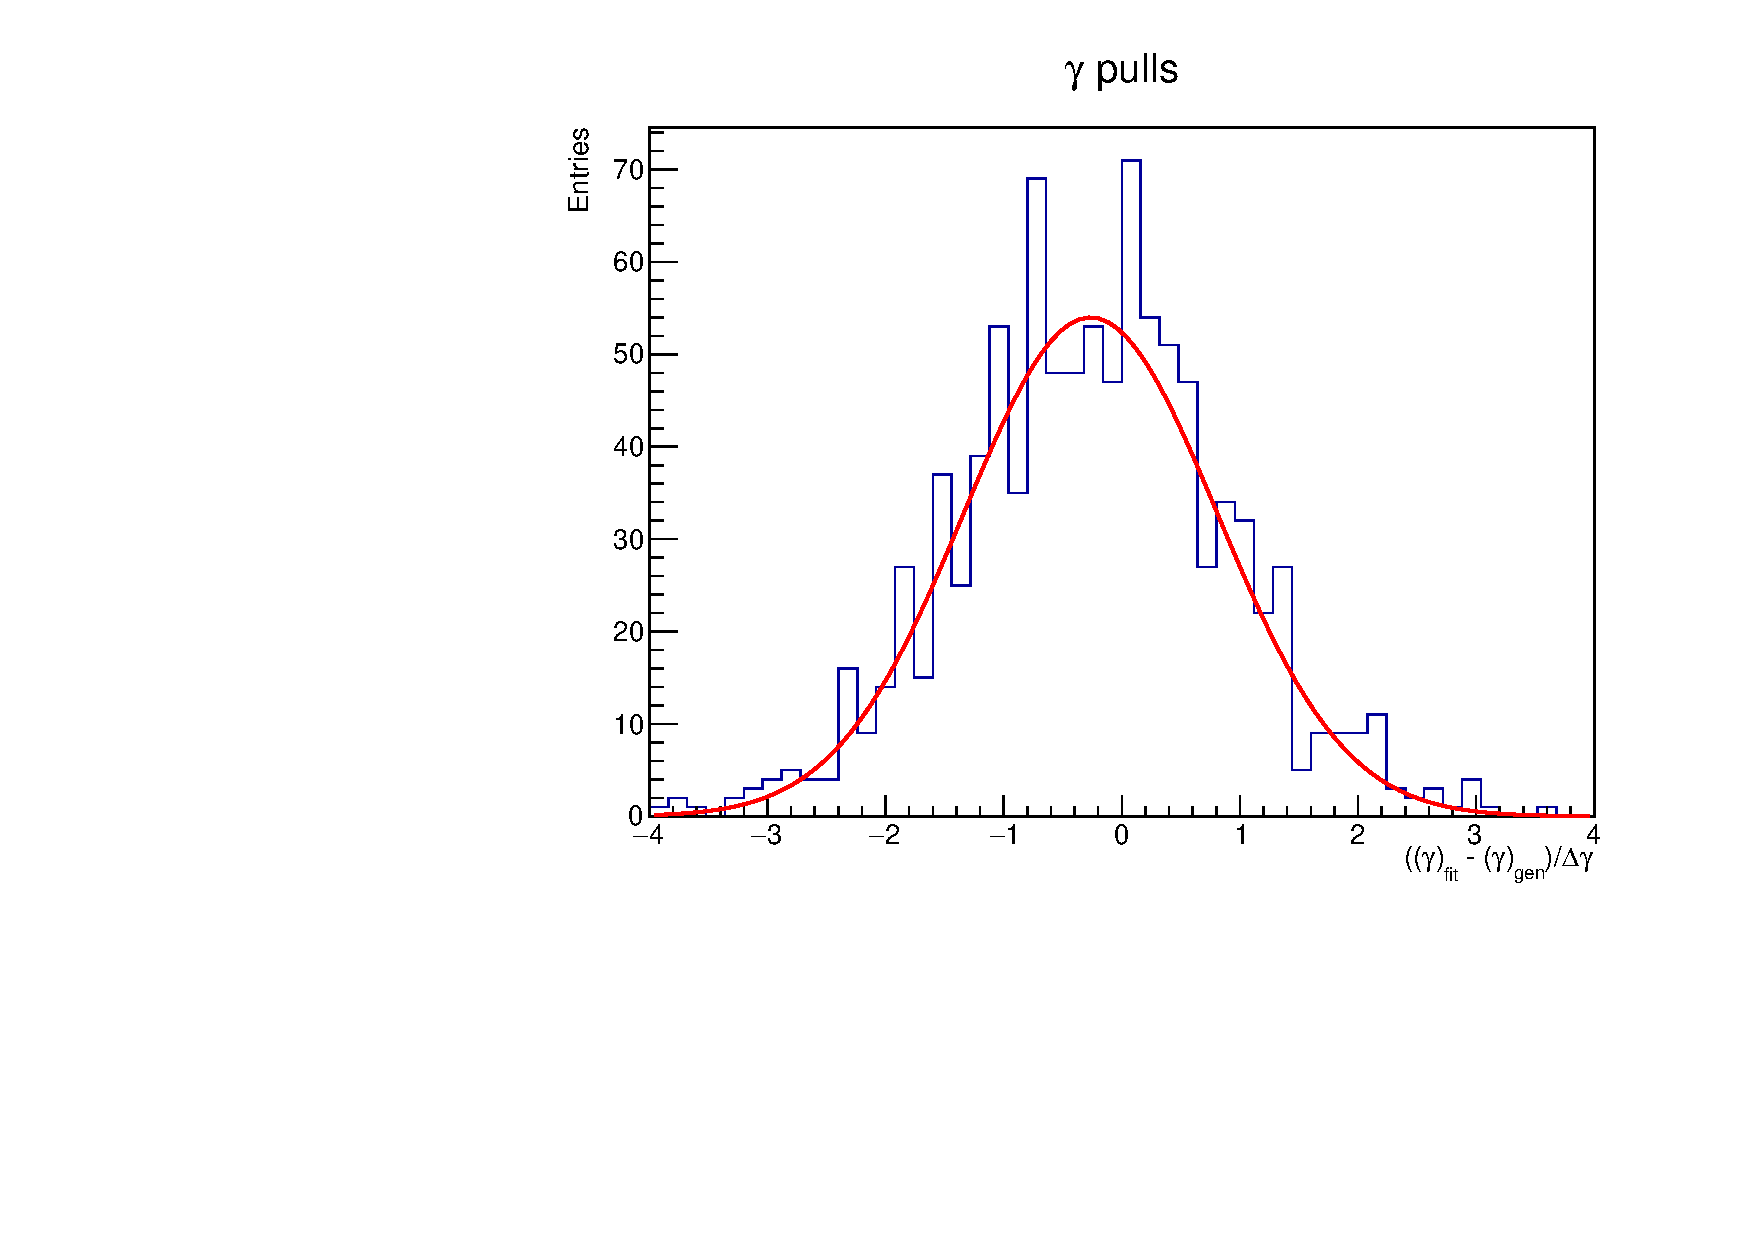
\includegraphics[width=1.0\textwidth]{Plots/gamma_pull_toys_pipipipi.pdf}
      \vspace{-0.3cm}
      \caption*{$\pi^+\pi^-\pi^+\pi^-$}
    \end{subfigure}
    \vspace{-0.5cm}
    \caption*{$\gamma$ pull distributions}
  \end{figure}
  \vspace{-0.3cm}
  \begin{center}
    Indeed, noticeable biases are observed!\\
    Use pull distributions to correct central values of physics parameters
  \end{center}
\end{frame}

\begin{frame}{Interpretation results}
  \begin{center}
    {\large Results from interpretation, after correcting for biases in central values (not uncertainties):}
  \end{center}
  \vspace{-0.5cm}
  \begin{columns}
    \begin{column}{0.5\textwidth}
      \begin{center}
        $K^+K^-\pi^+\pi^-$
      \end{center}
      \begin{align*}
        \gamma =& (117 \pm 15)^\circ \\
        \delta_B^{DK} =& (83 \pm 12)^\circ \\
        r_B^{DK} =& (12.1 \pm 2.6)\times10^{-2} \\
        \delta_B^{D\pi} =& (295 \pm 74)^\circ \\
        r_B^{D\pi} =& (0 \pm 5)\times10^{-3}
      \end{align*}
    \end{column}
    \begin{column}{0.5\textwidth}
      \begin{center}
        $\pi^+\pi^-\pi^+\pi^-$
      \end{center}
      \begin{align*}
        \gamma =& (45 \pm 11)^\circ \\
        \delta_B^{DK} =& (115 \pm 11)^\circ \\
        r_B^{DK} =& (8.2 \pm 1.9)\times10^{-2} \\
        \delta_B^{D\pi} =& (204 \pm 42)^\circ \\
        r_B^{D\pi} =& (4 \pm 5)\times10^{-3}
      \end{align*}
    \end{column}
  \end{columns}
  \vspace{0.3cm}
  \begin{center}
    It may seem like there is a huge tension still present...\\
    \phantom{...but how Gaussian are these uncertainties?}
  \end{center}
\end{frame}

\begin{frame}{Interpretation results}
  \begin{center}
    {\large Results from interpretation, after correcting for biases in central values (not uncertainties):}
  \end{center}
  \vspace{-0.5cm}
  \begin{columns}
    \begin{column}{0.5\textwidth}
      \begin{center}
        $K^+K^-\pi^+\pi^-$
      \end{center}
      \begin{align*}
        \gamma =& (117 \pm 15)^\circ \\
        \delta_B^{DK} =& (83 \pm 12)^\circ \\
        r_B^{DK} =& (12.1 \pm 2.6)\times10^{-2} \\
        \delta_B^{D\pi} =& (295 \pm 74)^\circ \\
        r_B^{D\pi} =& (0 \pm 5)\times10^{-3}
      \end{align*}
    \end{column}
    \begin{column}{0.5\textwidth}
      \begin{center}
        $\pi^+\pi^-\pi^+\pi^-$
      \end{center}
      \begin{align*}
        \gamma =& (45 \pm 11)^\circ \\
        \delta_B^{DK} =& (115 \pm 11)^\circ \\
        r_B^{DK} =& (8.2 \pm 1.9)\times10^{-2} \\
        \delta_B^{D\pi} =& (204 \pm 42)^\circ \\
        r_B^{D\pi} =& (4 \pm 5)\times10^{-3}
      \end{align*}
    \end{column}
  \end{columns}
  \vspace{0.3cm}
  \begin{center}
    It may seem like there is a huge tension still present...\\
    ...but how Gaussian are these uncertainties?
  \end{center}
\end{frame}

\begin{frame}{Likelihood scan of interpretation fit}
  \begin{center}
    In fact, a likelihood scan shows that $D\to K^+K^-\pi^+\pi^-$ and $D\to\pi^+\pi^-\pi^+\pi^-$ agree within $2\sigma$
  \end{center}
  \begin{figure}
    \centering
    \begin{subfigure}{0.50\textwidth}
      \centering
      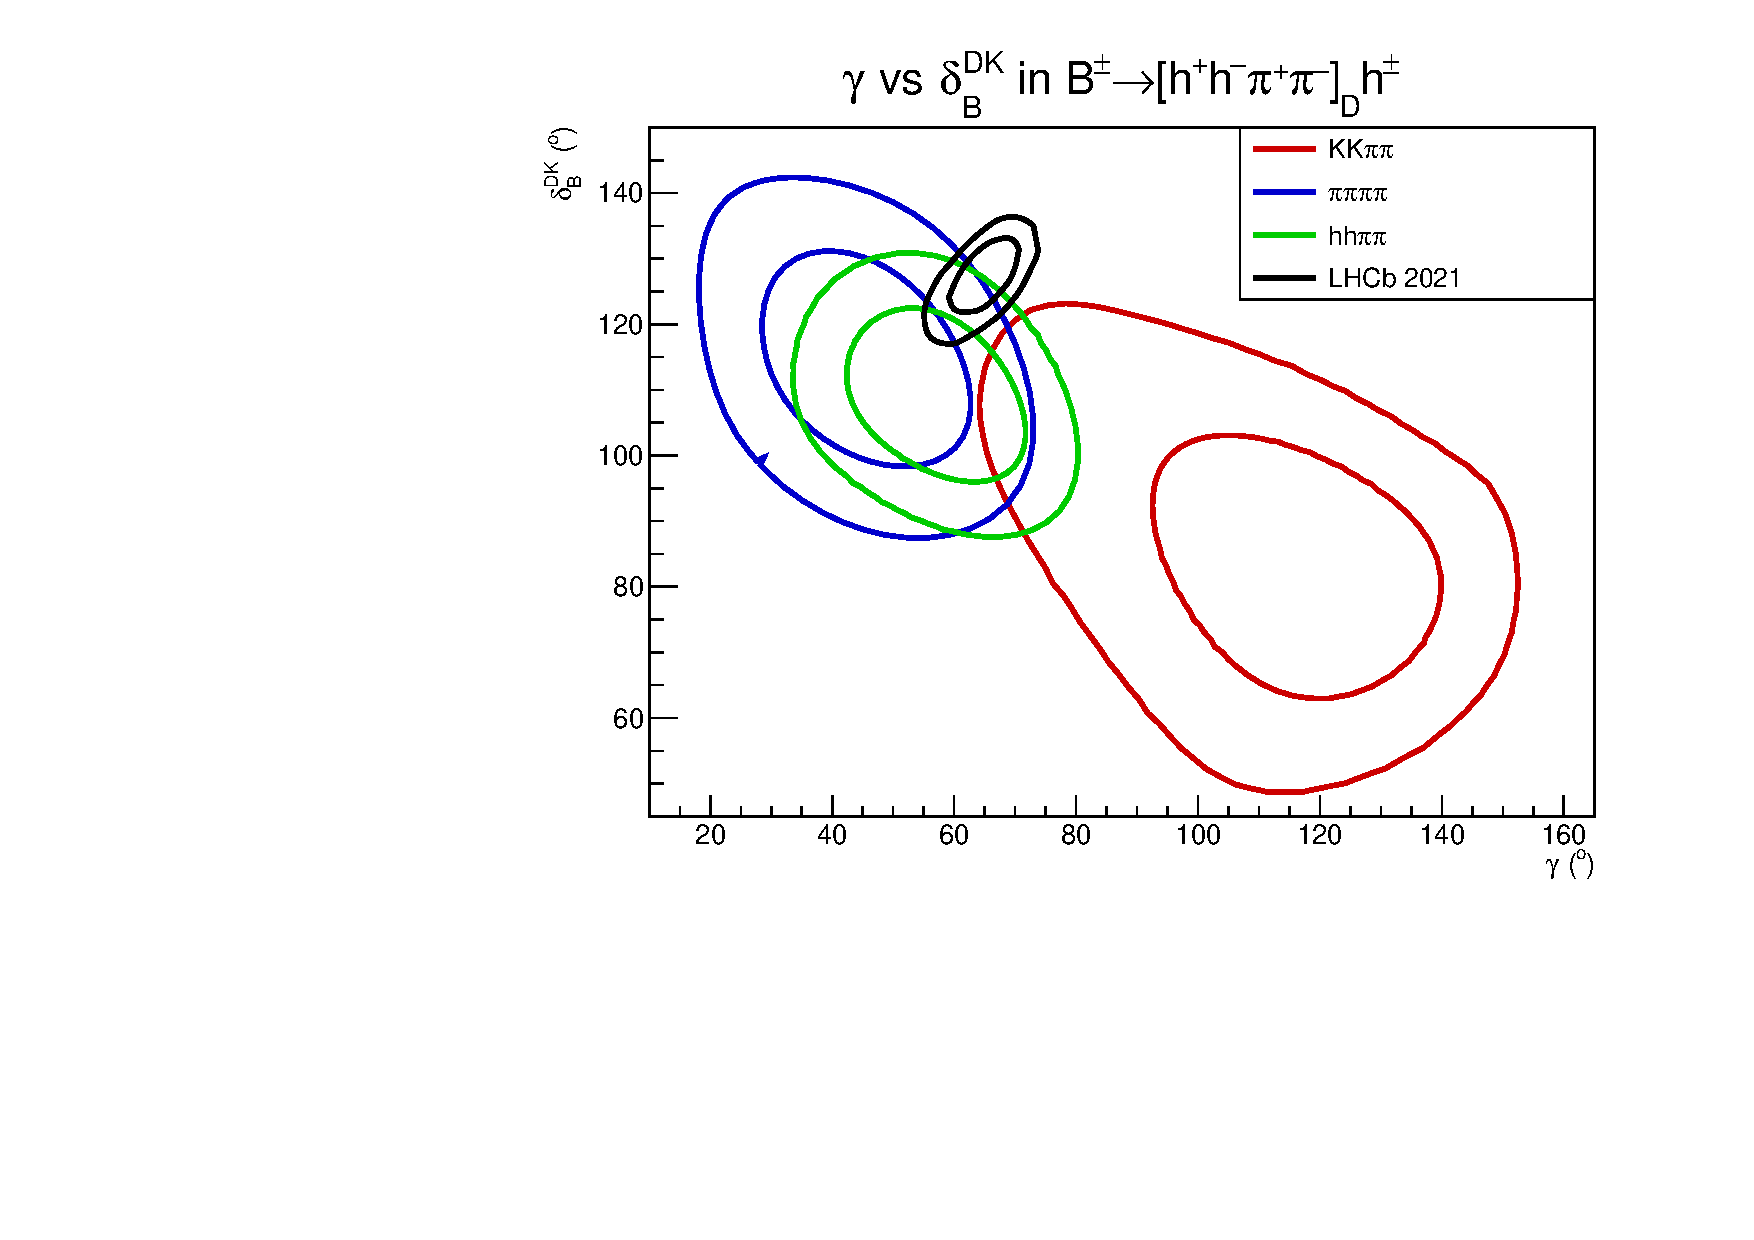
\includegraphics[width=1.0\textwidth]{Plots/gamma_deltaB_hhpipi_LHCb_Prob_scan.pdf}
      \caption*{$\gamma$ vs $\delta_B^{DK}$}
    \end{subfigure}%
    \begin{subfigure}{0.50\textwidth}
      \centering
      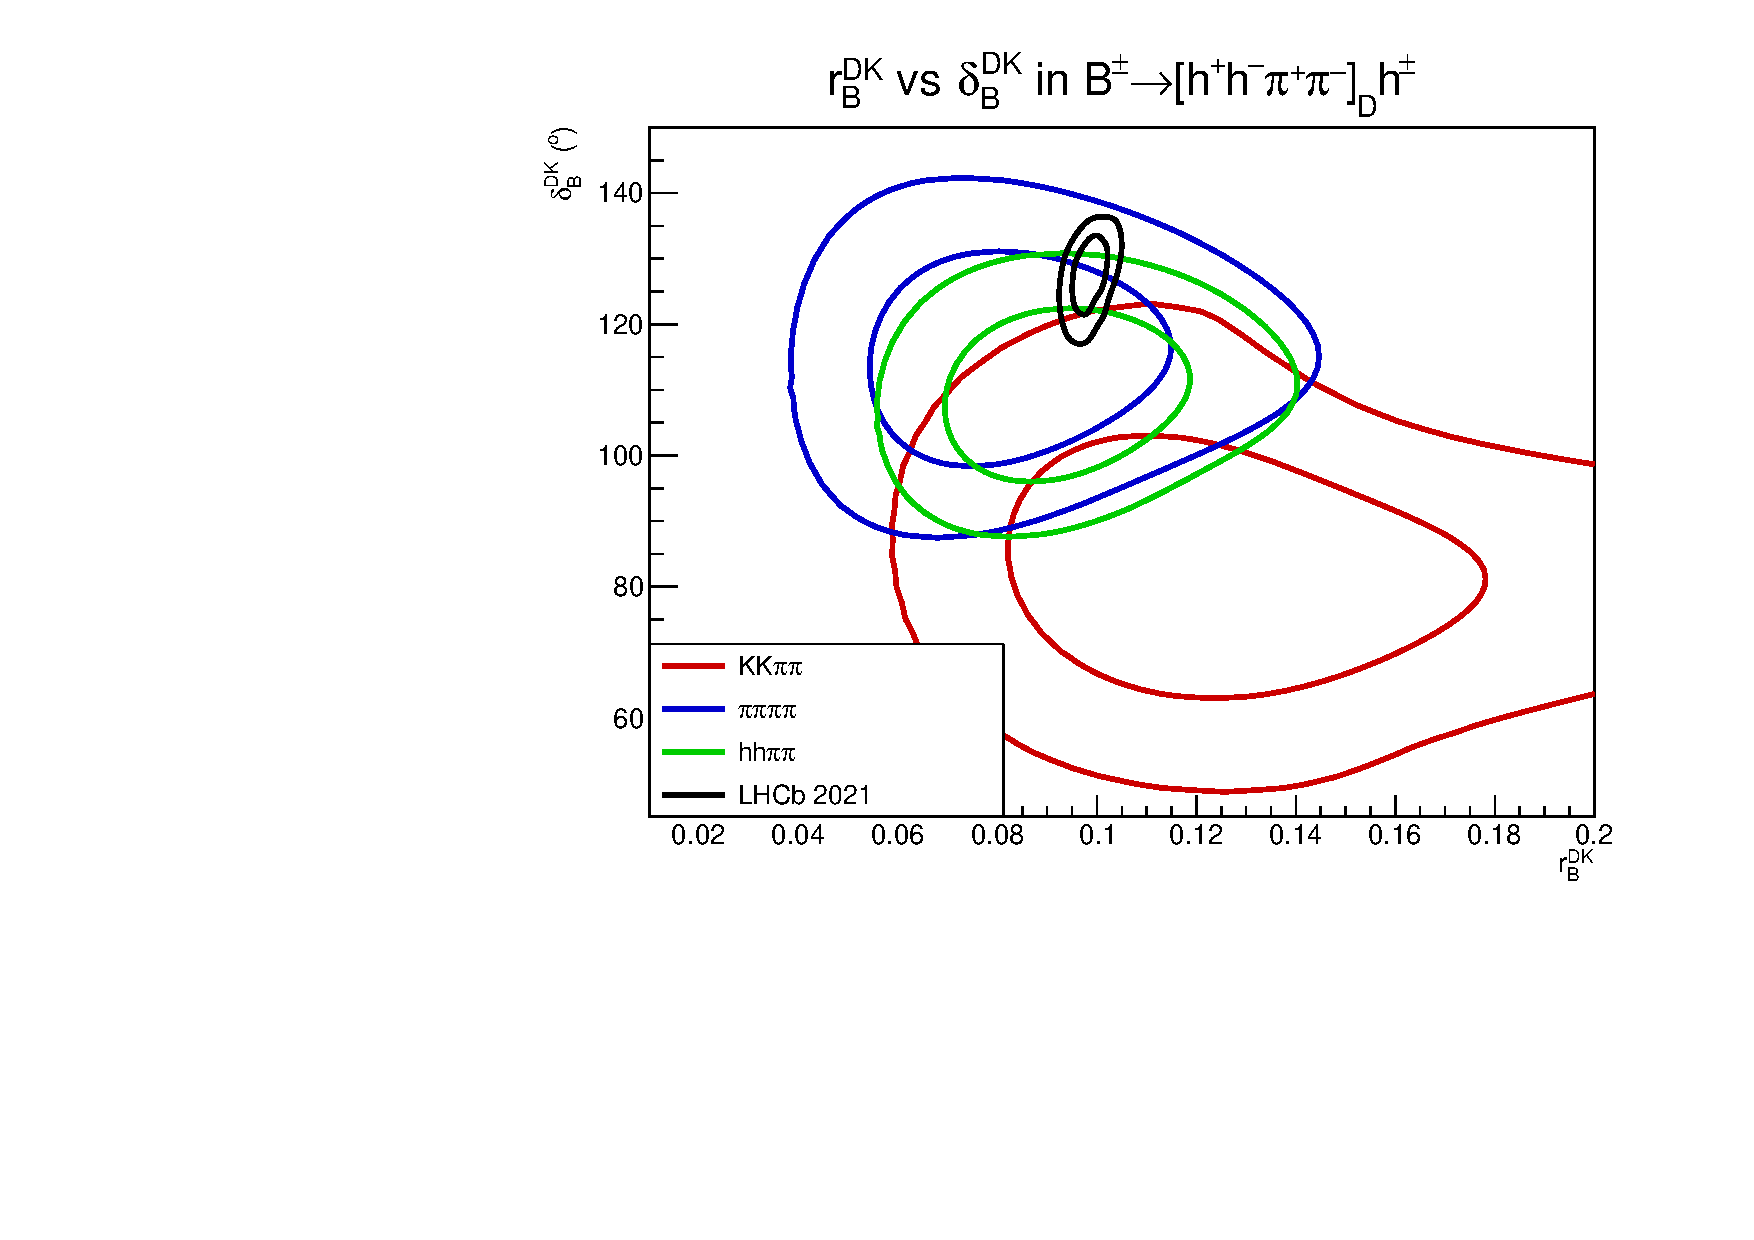
\includegraphics[width=1.0\textwidth]{Plots/rB_deltaB_hhpipi_LHCb_Prob_scan.pdf}
      \caption*{$r_B^{DK}$ vs $\delta_B^{DK}$}
    \end{subfigure}
  \end{figure}
  \vspace{-0.3cm}
  \begin{center}
    When all biases, correlations and non-Gaussian uncertainties are accounted for, the tension with the LHCb average has reduced significantly
  \end{center}
\end{frame}

\begin{frame}{Likelihood scan of interpretation fit}
  \begin{center}
    In fact, a likelihood scan shows that $D\to K^+K^-\pi^+\pi^-$ and $D\to\pi^+\pi^-\pi^+\pi^-$ agree within $2\sigma$
  \end{center}
  \begin{figure}
    \centering
    \begin{subfigure}{0.50\textwidth}
      \centering
      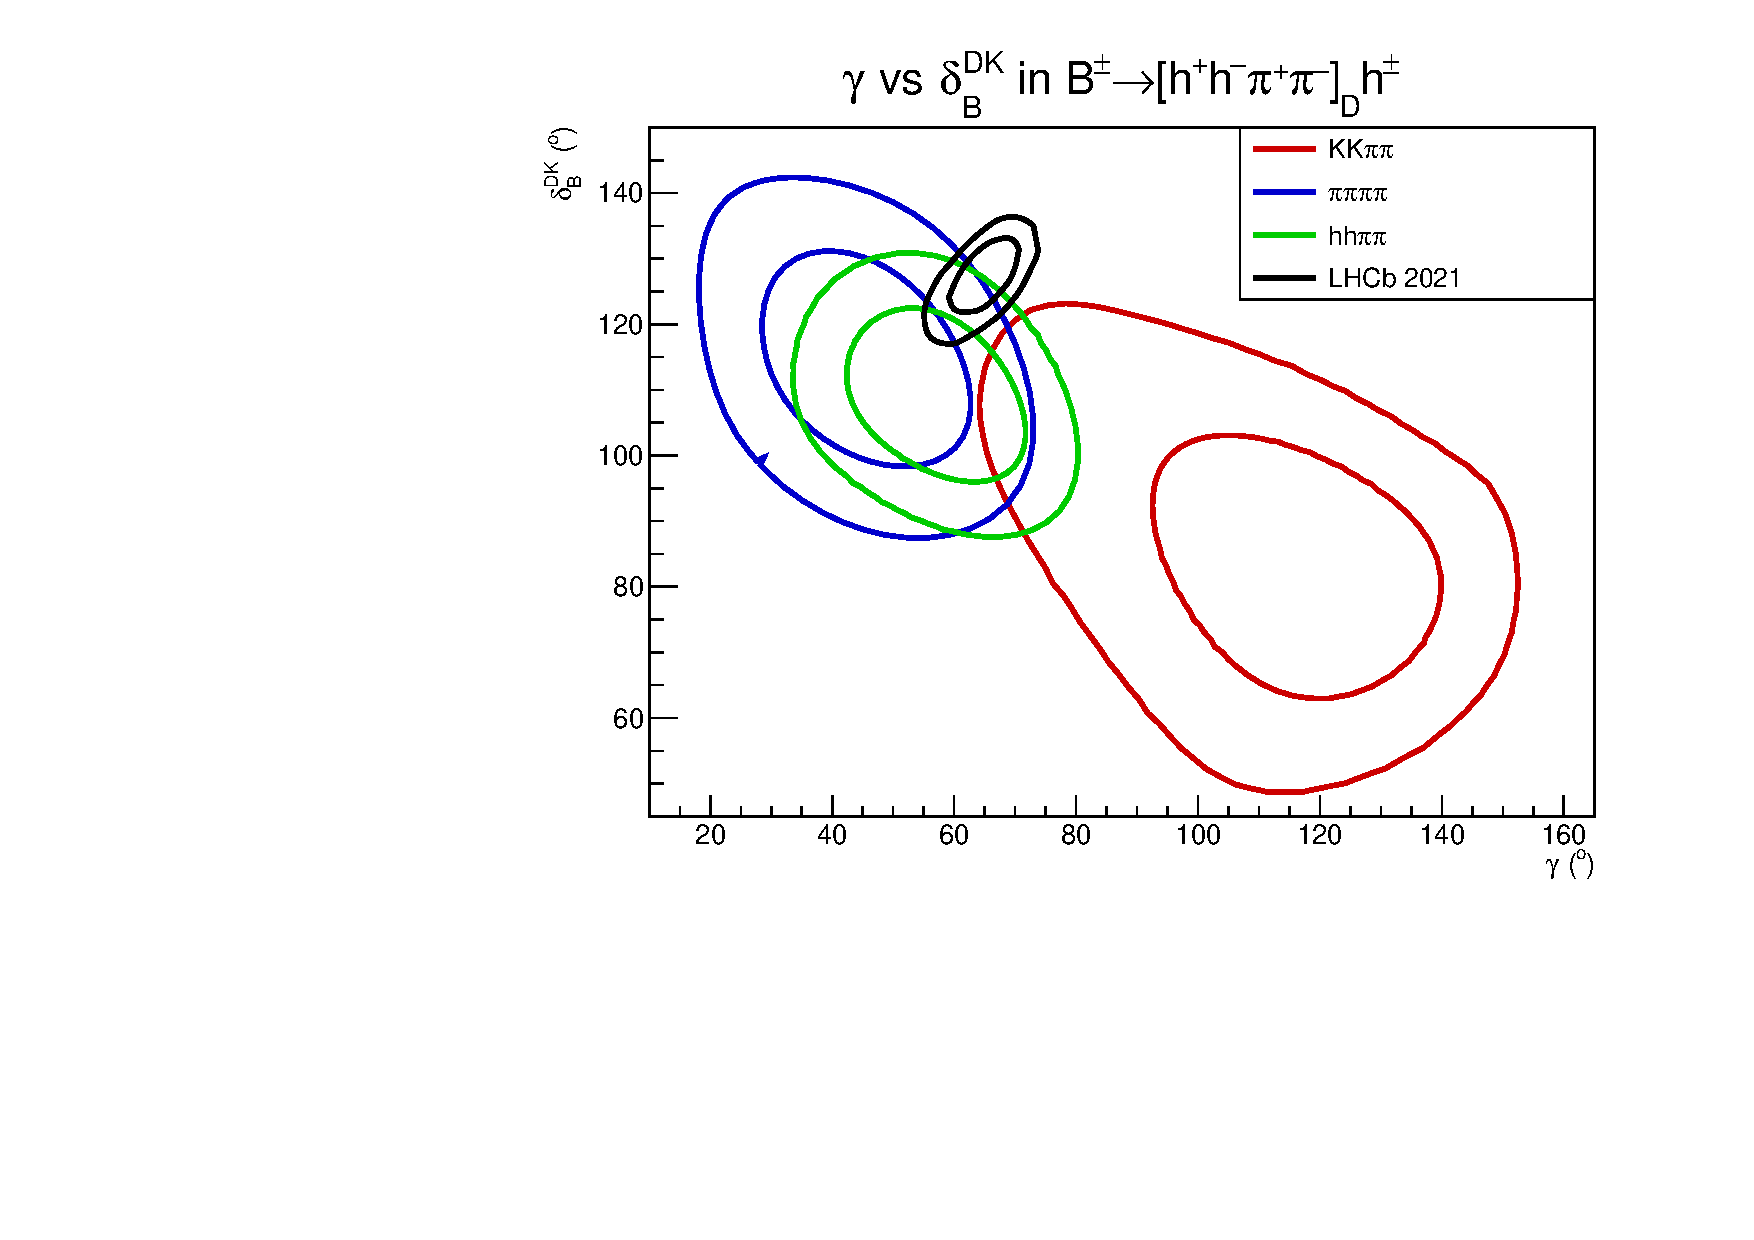
\includegraphics[width=1.0\textwidth]{Plots/gamma_deltaB_hhpipi_LHCb_Prob_scan.pdf}
      \caption*{$\gamma$ vs $\delta_B^{DK}$}
    \end{subfigure}%
    \begin{subfigure}{0.50\textwidth}
      \centering
      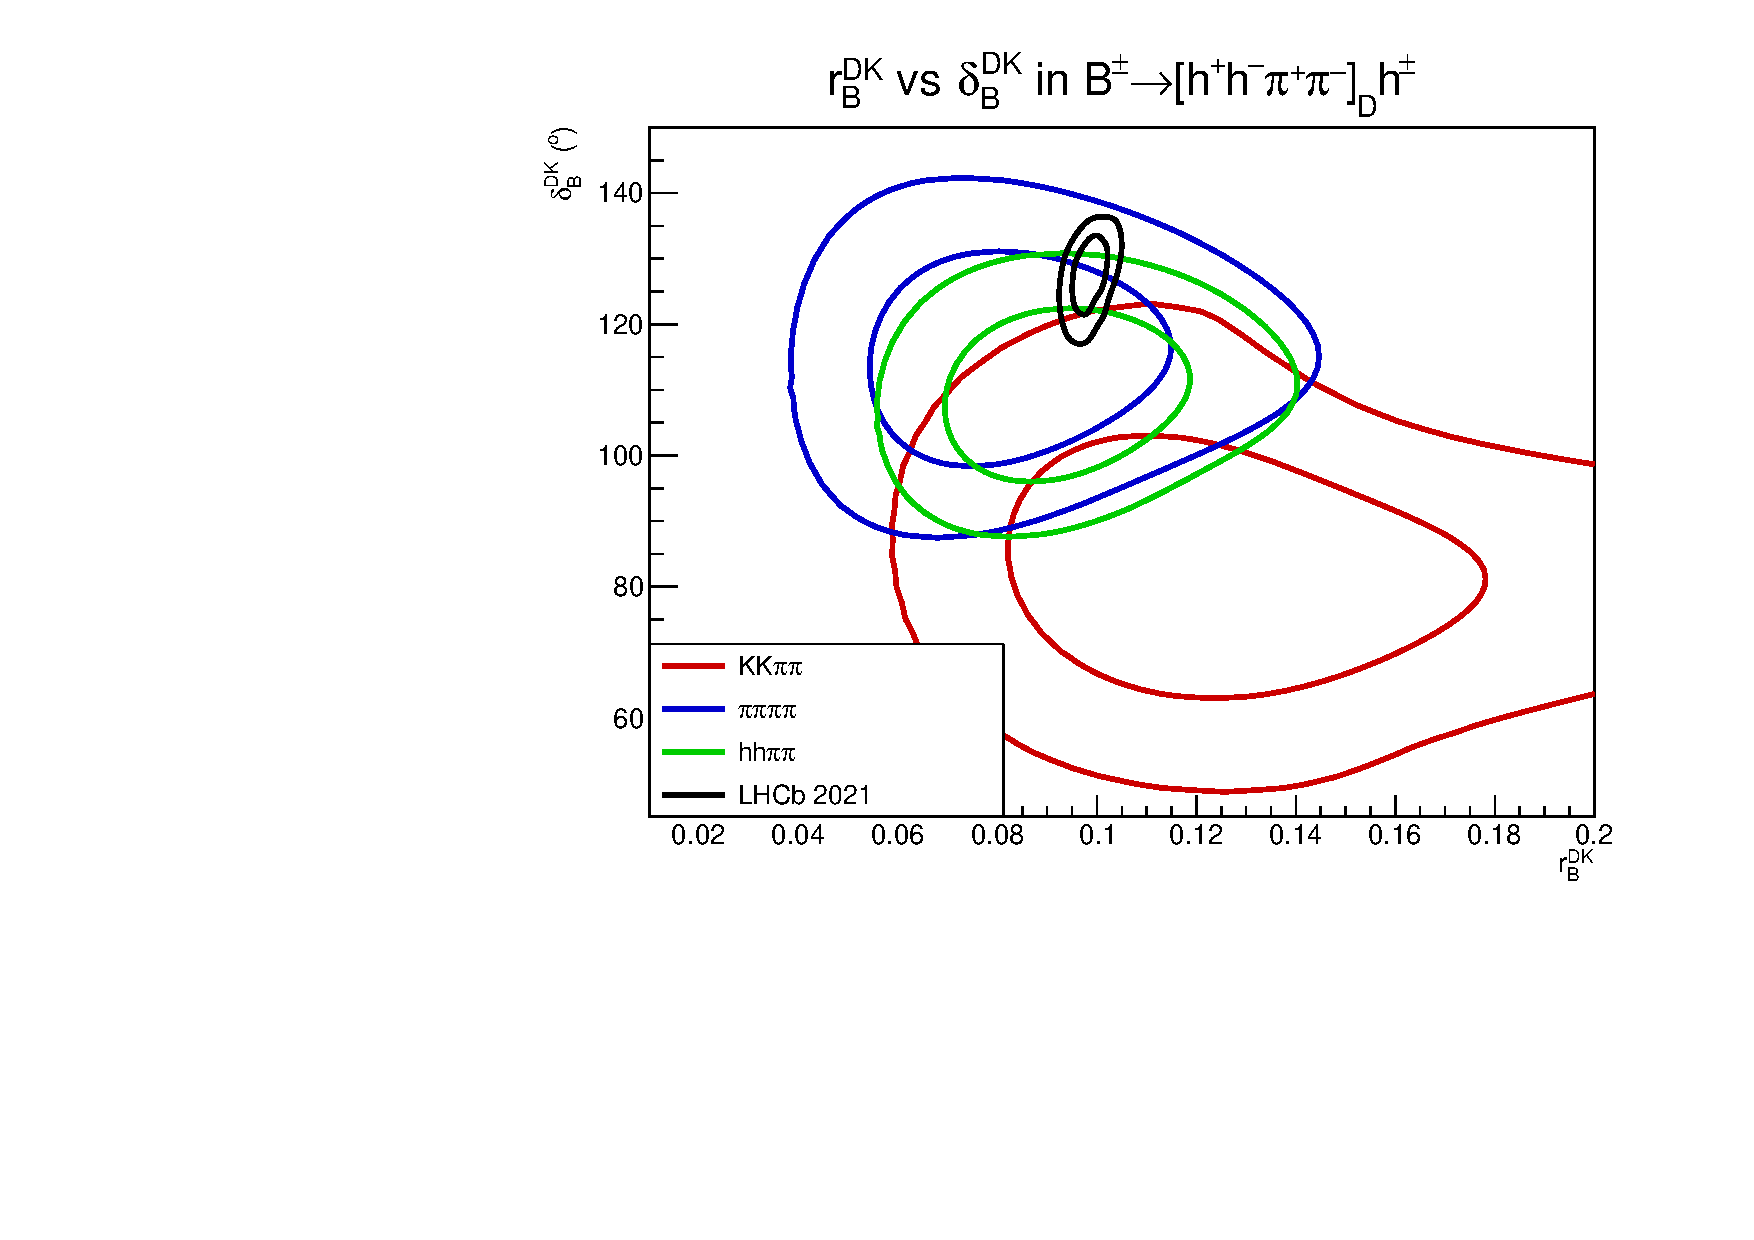
\includegraphics[width=1.0\textwidth]{Plots/rB_deltaB_hhpipi_LHCb_Prob_scan.pdf}
      \caption*{$r_B^{DK}$ vs $\delta_B^{DK}$}
    \end{subfigure}
  \end{figure}
  \vspace{-0.3cm}
  \begin{center}
    However, with all the non-Gaussian behaviour and asymmetric pull distributions, do we actually trust the uncertainties?
  \end{center}
\end{frame}

\begin{frame}{Plugin/Feldman-Cousins method}
  \begin{center}
    {\Large Feldman-Cousins method, or Plugin, is a ``brute-force'' approach to assigning a confidence interval} \\~\\
    {At each scan point of $\gamma$, perform these fits to data:}
  \end{center}
  \begin{enumerate}
    \setlength\itemsep{0.5em}
    \item{Fit with all parameters floating, and save the log-likelihood $\chi^2$}
    \item{Fit with $\gamma$ fixed to scan point, and save $\chi^2_{\rm fix}$}
    \item{Calculate $\Delta\chi^2_{\rm data} = \chi^2_{\rm fix} - \chi^2$}
  \end{enumerate}
  \vspace{0.5cm}
  \begin{center}
    {We expect $\Delta\chi^2_{\rm data}$ to become large as we move away from best-fit value, but without direct knowledge of underlying PDF, we cannot determine any confidence intervals from this}
  \end{center}
\end{frame}

\begin{frame}{Plugin/Feldman-Cousins method}
  \begin{center}
    {\Large Feldman-Cousins method, or Plugin, is a ``brute-force'' approach to assigning a confidence interval} \\~\\
    {At each scan point of $\gamma$, perform these fits to toy:}
  \end{center}
  \begin{enumerate}
    \setlength\itemsep{0.5em}
    \item{Fix $\gamma$ to scan point and generate $1000$ toys}
    \item{Perform fits to each toy, with $\gamma$ both floating and fixed}
    \item{Calculate $\Delta\chi^2_{\rm toy}$}
  \end{enumerate}
  \vspace{0.42cm}
  \begin{center}
    {At each scan point, the fraction of toys with $\Delta\chi^2_{\rm toy} > \Delta\chi^2_{\rm data}$ is equal to $1 - \rm{CL}$, and the exact $68\%$ confidence interval can then be obtained using an interpolation between points}
  \end{center}
\end{frame}

\begin{frame}{Plugin/Feldman-Cousins method}
  \begin{center}
    Combined fit shows good agreement between Plugin and Prob scans \\
    As expected, $D\to K^+K^-\pi^+\pi^-$ shows a large non-Gaussian tail
  \end{center}
  \begin{figure}
    \centering
    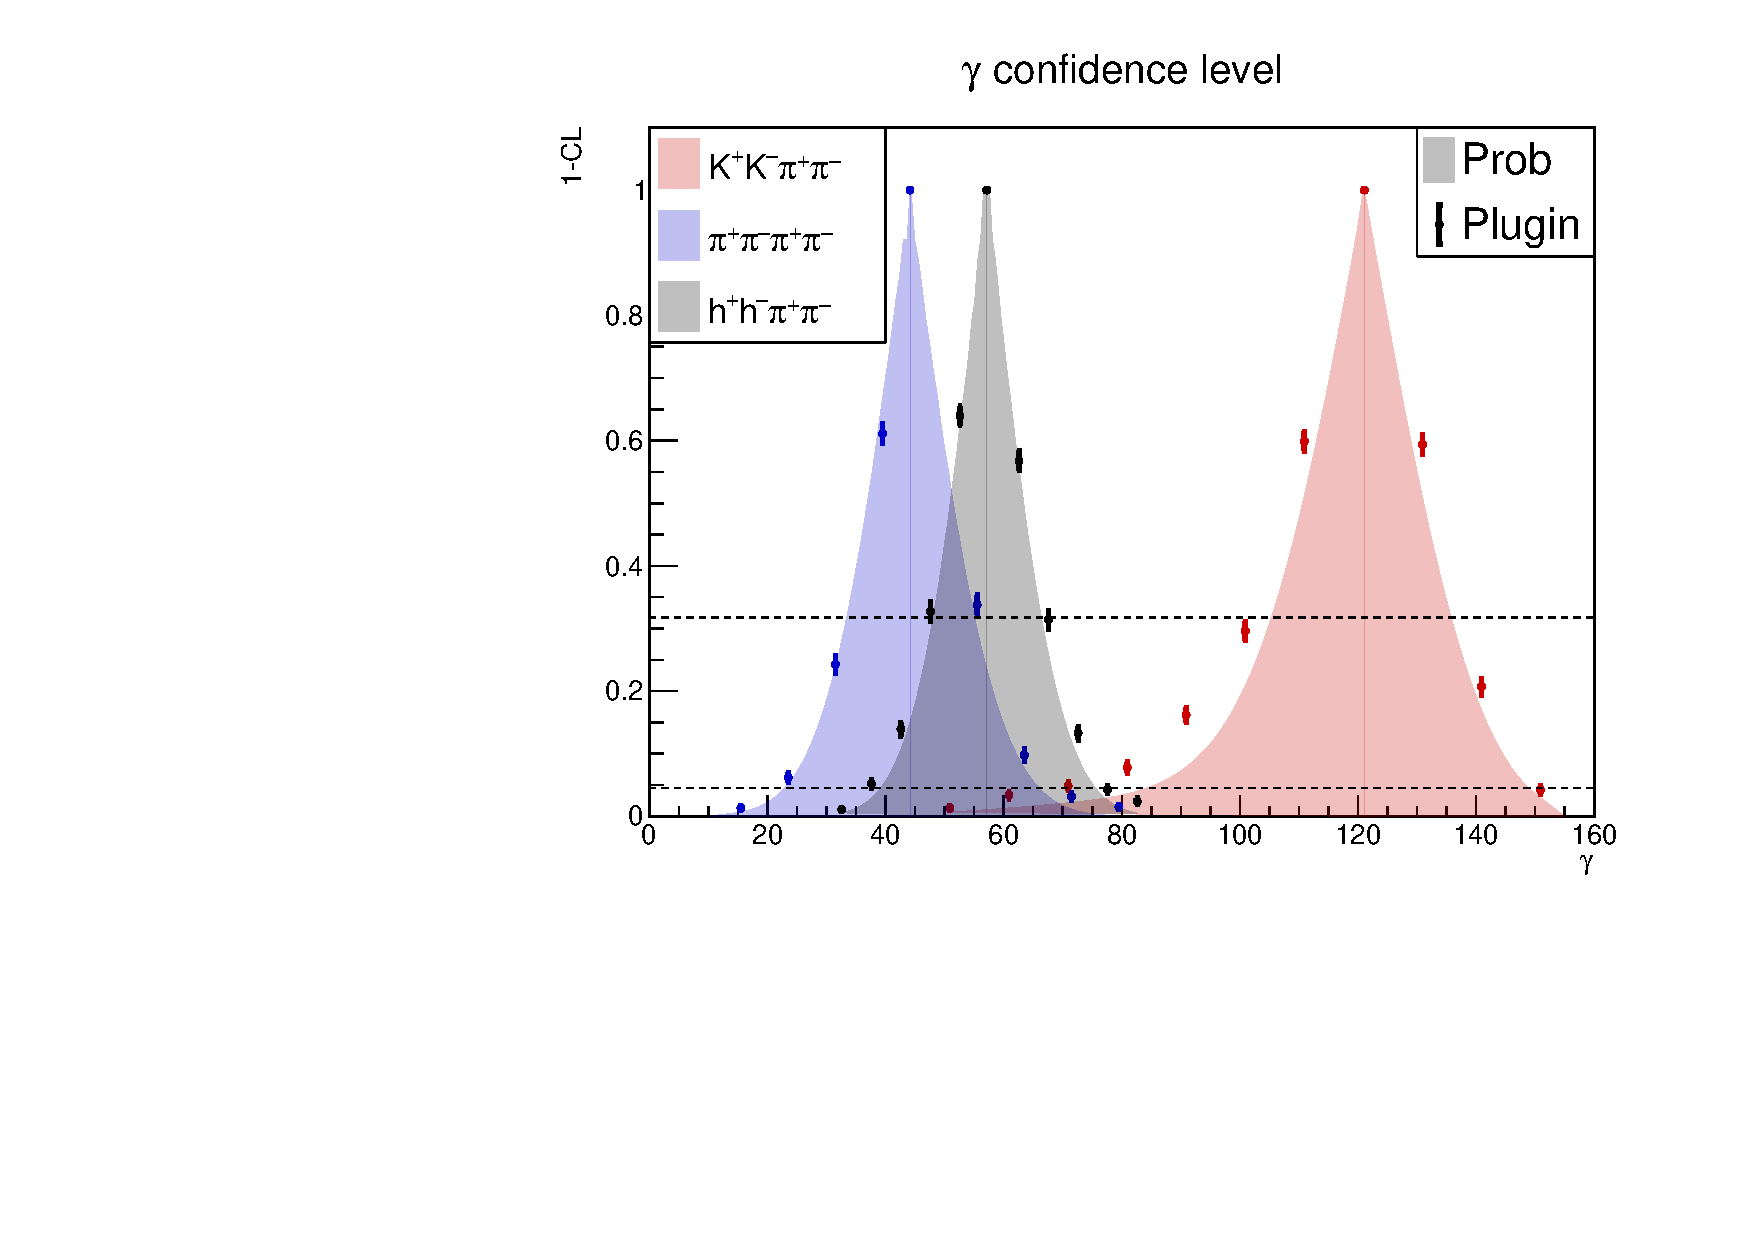
\includegraphics[width=0.6\textwidth]{Plots/gamma_plugin_scan.pdf}
  \end{figure}
  \vspace{-0.3cm}
  \begin{center}
    Combined fit result: $\gamma = (57 \pm 9)^\circ$\\
    Third most precise single measurement of $\gamma$ {\color{blue}(need to double check this)}
  \end{center}
\end{frame}

\section{Conclusion}
\begin{frame}{Conclusion}
  \begin{itemize}
    \setlength\itemsep{1.0em}
    \item{Model-independent measurement of $\gamma$ with $B^\pm\to[h^+h^-\pi^+\pi^-]_Dh^\pm$ has been performed: $\gamma = (57 \pm 9)^\circ$}
    \item{$3\sigma$ tension in $D\to K^+K^-\pi^+\pi^-$ has reduced to less than $2\sigma$ due to:}
    \begin{enumerate}
      \item{Non-Gaussian uncertainties in $y_\pm^{DK}$ originating from $s_i$ uncertainties}
      \item{Large anti-correlation between $\gamma$ and $\delta_B^{DK}$}
    \end{enumerate}
    \item{First $\gamma$ measurement using $D\to\pi^+\pi^-\pi^+\pi^-$}
    \item{Statistically limited measurement, but $s_i$ uncertainties are large}
    \begin{itemize}
      \item{Charm mixing studies will improve this!}
    \end{itemize}
    \item{The ANA note is ready, and we would like to start B2OC WG review}
  \end{itemize}
  \begin{center}
    {\huge Thanks for your attention!}
  \end{center}
\end{frame}

\begin{frame}{Backup: Charm mixing studies with multi-body decays}
  \begin{center}
    {\large Sensitivity to $c_i$: Similar between BESIII and charm mixing at LHCb}
  \end{center}
  \begin{figure}[htb]
    \centering
    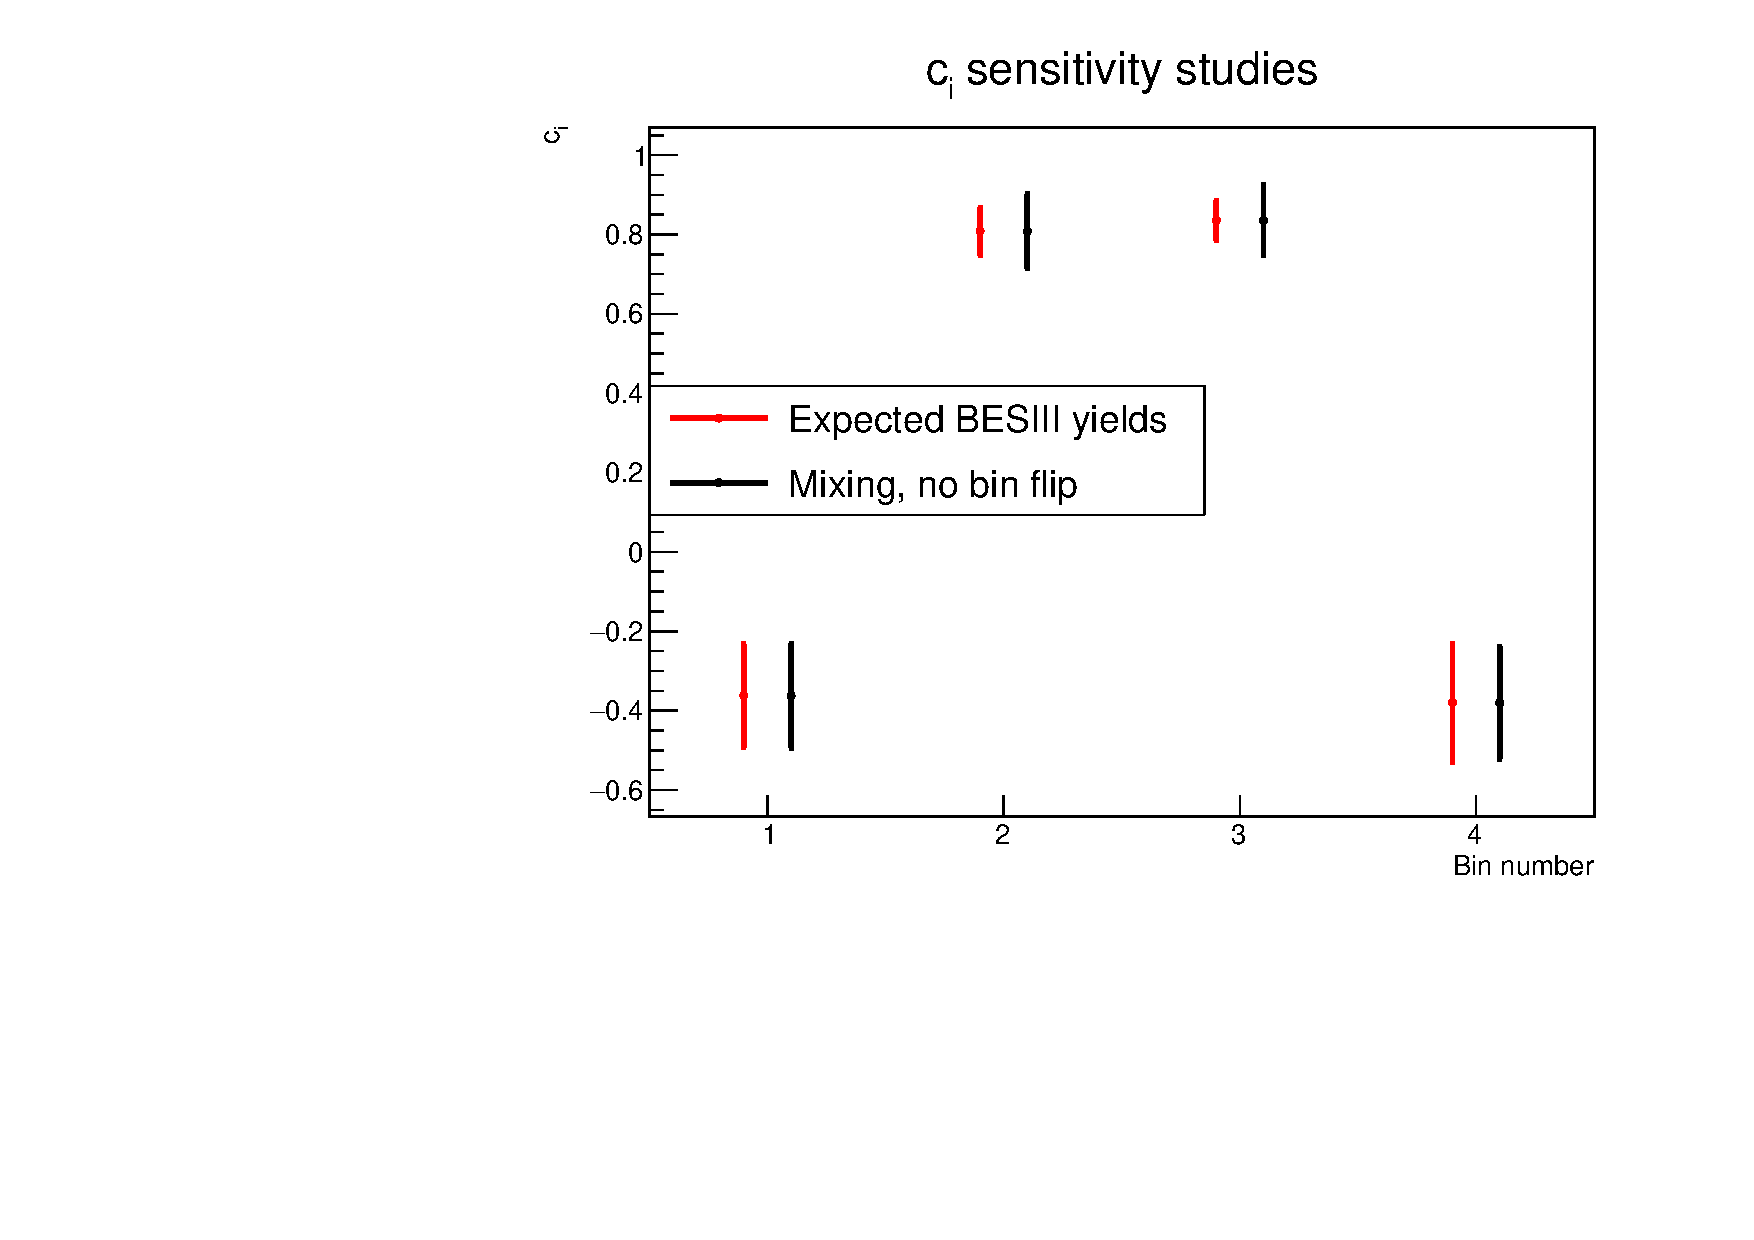
\includegraphics[width=0.7\textwidth]{Plots/ci_sensitivity.pdf}
  \end{figure}
  \vspace{-0.4cm}
  \begin{itemize}
    \item{BESIII yields equivalent to $\SI{8}{\per\femto\barn}$ of $\psi(3770)$}
    \item{4 million $D\to K^+K^-\pi^+\pi^-$ candidates in mixing analysis}
    \end{itemize}
\end{frame}

\begin{frame}{Backup: Charm mixing studies with multi-body decays}
  \begin{center}
    {\large Sensitivity to $s_i$: Significant improvements expected!}
  \end{center}
  \begin{figure}[htb]
    \centering
    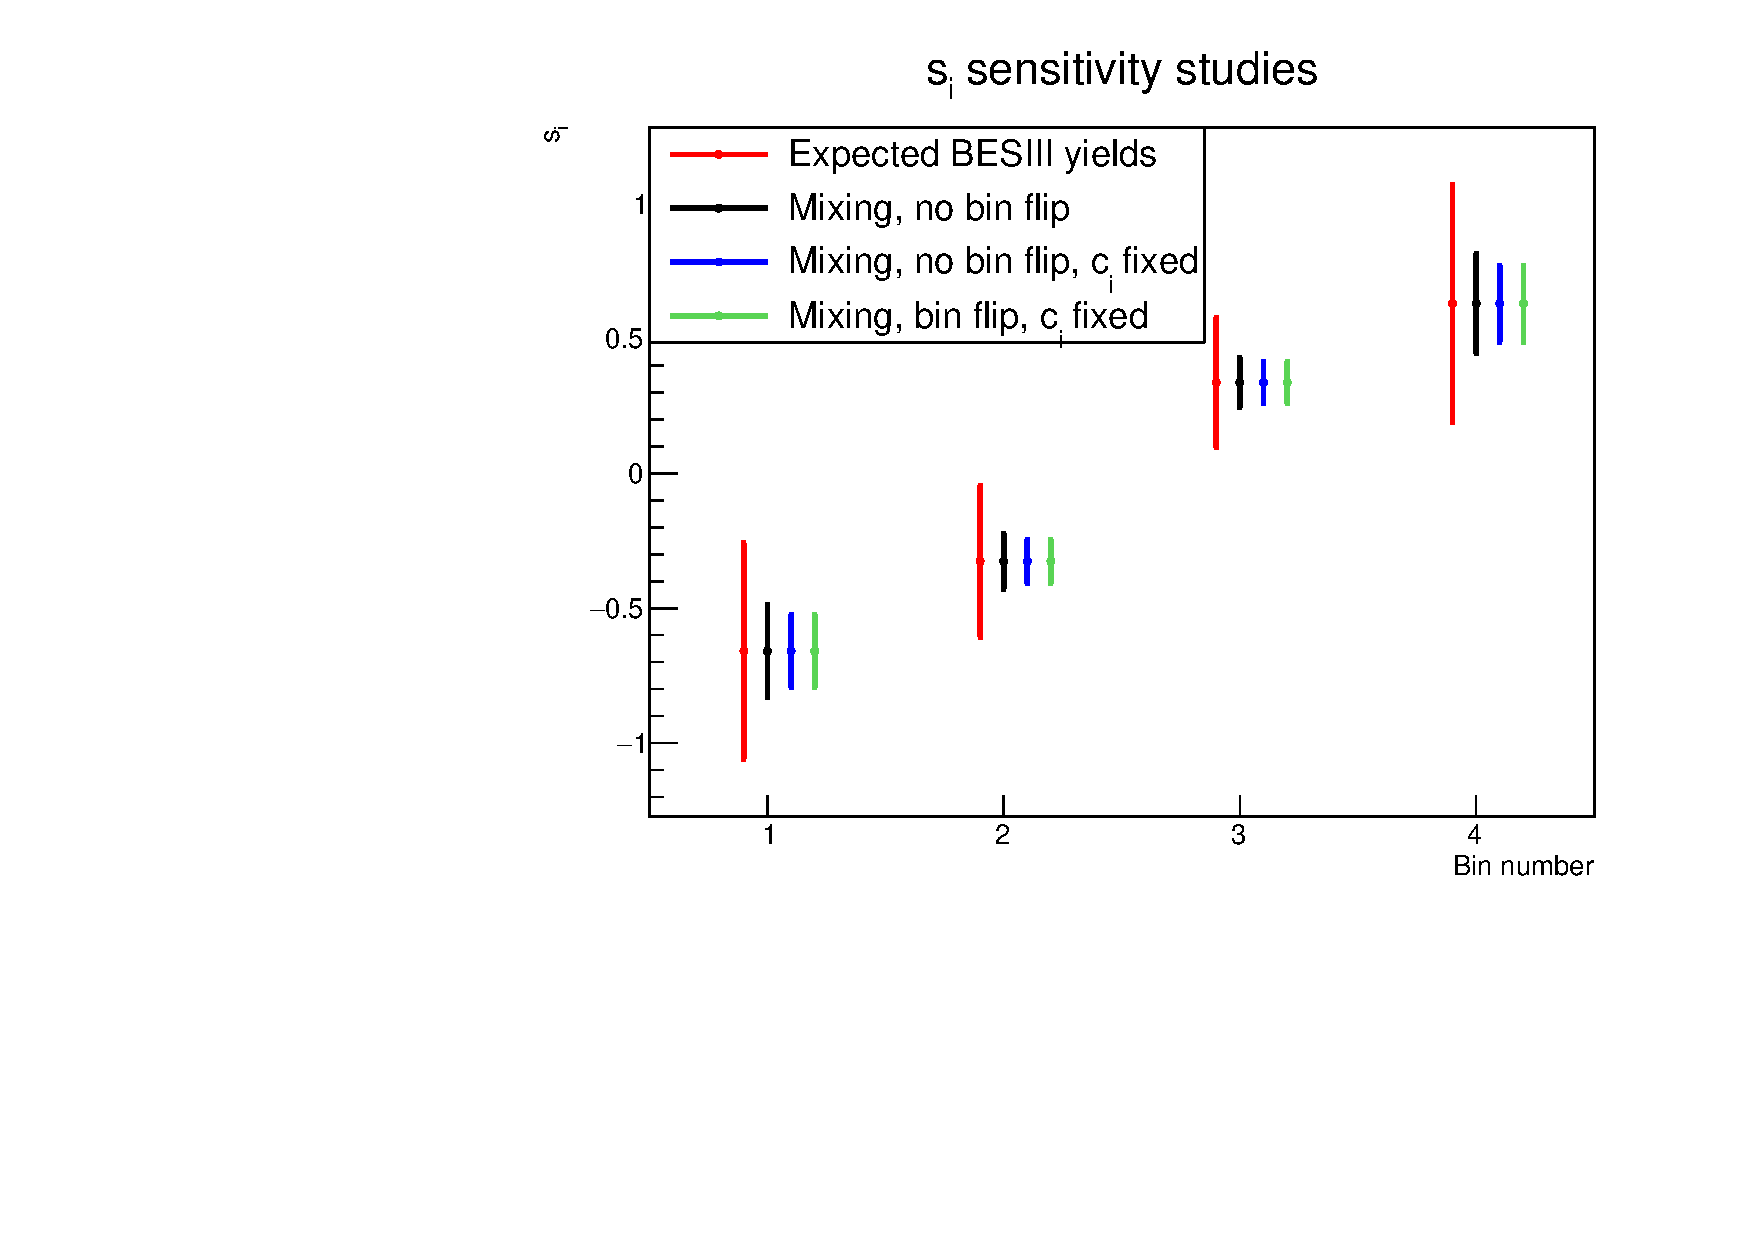
\includegraphics[width=0.7\textwidth]{Plots/si_sensitivity.pdf}
  \end{figure}
  \vspace{-0.4cm}
  \begin{itemize}
    \item{BESIII yields equivalent to $\SI{8}{\per\femto\barn}$ of $\psi(3770)$}
    \item{4 million $D\to K^+K^-\pi^+\pi^-$ candidates in mixing analysis}
  \end{itemize}
\end{frame}

\end{document}
